\documentclass[12pt]{article}
\usepackage[myheadings]{fullpage}

% You can remove this line as it's not needed for your purpose.
%\DeclareUnicodeCharacter{0301}{\hspace{-1ex}\'{ }}

% For figures and stuff
\usepackage{graphicx, wrapfig, subcaption, setspace, booktabs, wrapfig}
\usepackage[T1]{fontenc}
\usepackage{helvet}

% Maths
\usepackage{amsmath, amssymb}
\usepackage{float}

% Language and font encodings
\usepackage[utf8]{inputenc}
\usepackage[english]{babel}
\usepackage{csquotes}

% Package for headers
\usepackage{fancyhdr}
\pagestyle{fancy}
\fancyhf{}
\fancyfoot[C]{\thepage}
\usepackage{lastpage}

% setting document style
\setlength{\parindent}{0mm}
\setlength{\parskip}{1.5mm}
\newcommand{\noappendixindent}{
    \setlength{\parindent}{0pt}
}
%% Sets page size and margins
\usepackage[a4paper,top=2.5cm,bottom=2.5cm,left=2cm,right=2cm,marginparwidth=1.5cm]{geometry}


% Change for different font sizes and families
\usepackage[font=small, labelfont=bf]{caption}
\usepackage{fourier}
\usepackage[protrusion=true, expansion=true]{microtype}


% Bibliography
\usepackage{bookmark}
\usepackage[backend=biber, style=nature, sorting=none, doi=false, isbn=false, date=year, url=false]{biblatex}



% Packages for tables and units
\usepackage{wrapfig}
\usepackage{booktabs} % For \toprule, \midrule, and \bottomrule
\usepackage{siunitx}  % Formats the units and values
\usepackage[version=4]{mhchem}
\usepackage{textcomp}
\usepackage{pgfplots}
\usepackage{pgfplotstable} % Generates table from .csv
\pgfplotsset{compat=1.18}
\usepackage{array} % for new column definition
\usepackage{multirow}
\usepackage{threeparttable}
\usepackage{indentfirst}
\usepackage{wrapfig}
\usepackage[euler]{textgreek}
\usepackage{float}


% Hyperlink settings
\usepackage{hyperref}
\hypersetup{
    colorlinks=true,
    linkcolor=black,
    filecolor=green,      
    urlcolor=teal,
    citecolor=teal,
}

\graphicspath{{./thesis_pictures/}}
\addbibresource{bib/references_lib.bib}

\begin{document}
\setlength{\parindent}{0.5cm}
\emergencystretch=1em
\setstretch{1.15}

\begin{titlepage}\label{sec:title}
    \phantomsection
    \newgeometry{top=4cm}
    \begin{center}
    \thispagestyle{empty}
    
    \Large
    Research Report\\
    \vspace{0.2cm}
    \huge{Phylogenetically-Constrained\\Metabolic Network Expansion}
    %\vspace{0.5cm}
    

    
\includegraphics[scale=0.35]{logo/title_logos}

    
    \vspace{0.8cm}
    \large\textbf{Dimitra Astra Demertzi}\\
    \vspace{0.2cm}
    \large Under the supervision of\\ \emph{prof. dr. Shawn E. McGlynn}\\ and \emph{prof. dr. Wilhelm T.S. Huck}
    \vspace{3cm}
    

    \normalsize
    Earth-Life Science Institute | Tokyo Institute of Technology
    \\
    Department of Physical Organic Chemistry |  Faculty of Science | Radboud University
    \\
    \normalsize\textbf{2024}
    
    \vfill
    \end{center}
    \end{titlepage}
%\newpage
\begin{center}
    \thispagestyle{empty}
    \vspace*{\fill}
    \large\emph{This is acknowledgement}
    \vspace*{\fill}
\end{center}

%\newpage
\thispagestyle{empty}
\section*{\textbf{Abstract}}

\large 

We hypothesize that the MNE algorithm's nature is predetermined rather than evolution-like. Our phylogenetically constrained analysis demonstrates that the expansion process depends entirely on the nature, topology, and number of seeds used, reflecting the flow of chemical information within the network.

Here, we explore the nature of MNE by reconstructing metabolic networks of the Last Archaeal Common Ancestor (LACA) for multiple datasets of varying taxonomic resolution, and investigate the effect of taxon sampling on the expansion process. We hypothesize that the expansion process is predetermined rather than evolution-like, and that the flow of chemical information within the network is solely dependent on the nature, topology, and number of seeds used for expansion.

\newpage
\tableofcontents
\thispagestyle{empty}

\newpage
\section{Introduction}
\normalsize
Outline
\begin{itemize}
    \item OF, OFs, orthologs, paralogs, etc
    \item evolutionary models: DTL vs DLC
    \item HMMs \& advantage of position-independent evolutionary models
    \item Metabolic network expansion -> more? what is it, what are the models, etc.
    \item Metabolic network expansion traditionally used to infer evolution of metabolism. Study objective. Essentially connecting phylogenetic analysis with met. net. exp.
\end{itemize}


\subsection*{A surge in available data}
\addcontentsline{toc}{subsubsection}{A surge in available data}

The advancement of sequencing technologies and the development of state-of-the-art bioinformatics tools have enabled a rapid increase not only in the number of sequenced genomes, but also in the sampled prokaryotic diversity, expanding our view of the tree of life, and especially that of the archaeal branch. This surge in data availability can readily improve the resolution of modern phylogenetic relationships, resolve further their deep evolutionary history, and provide more accurate inference of ancestral gene contents \cite{tahon2021}. The first release of GTDB back in 2019, R89, contained 145,904 genomes organized into 24,706 species clusters, while its latest, R220 release this April, has grown to contain 596,859 genomes organized into 113,104 species clusters \cite{parks2018, parks2020, parks2022, rinke2021}; an increase of more than 300\% in just five years.

To date, several studies have investigated the nature and physiology of LACA, LBCA, and LUCA (Last Universal Common Ancestor) through gene content estimation \cite{williams2017, xavier2021, moody2024, coleman2021}, with datasets of various sizes and microbial physiologies, originating from a number of different databases. Usually these datasets are optimized for tree rooting and take into account taxon sampling evenness, yet it is still unclear how the incorporation of more species or other species belonging to the same higher taxonomic level will affect the analysis.
 
Moreover, GTDB, in its effort to standardize prokaryotic taxonomy, employs rank-normalization for the classification of microorganisms at all taxonomic levels \cite{parks2018}, which leads to periodic reclassification and renaming of taxa in the database. The change in nomenclature and the constant taxonomic revisions create confusion even when referencing taxa from the same database, and hinder the refinement of deep phylogenetic relationships \cite{tahon2021}. Especially in an era of exponential growth in genomic data, there is a pressing need to determine the robustness of standard methodologies and result stability. 
\section{Methods}


\subsection*{Data Retrieval \& Datasets Establishment}
\addcontentsline{toc}{subsubsection}{Data Retrieval \& Datasets Establishment}
We obtained the amino acid FASTA files containing all protein-encoding gene sequences predicted with Prodigal \cite{hyatt2010a} for all representative archaeal and bacterial species, from the Genome Taxonomy Database (GTDB, release R08-RS214, accessed in March 2024) \cite{parks2018, parks2020, parks2022, rinke2021} 

As of March 2024, the database contained 402,709 genomes organized into 85,205 species clusters, with one representative genome of each named species, according to Parks et al. (2020) \cite{parks2020}. We kept only the genomes which met the high quality completeness ($\geq$  90\%) and low contamination ($\leq$ 5\%) criteria, as defined by MIMAG \cite{thegenomestandardsconsortium2017}. Out of the 85,205 (4,416 archaeal and 80,789 bacterial) representative (REP) genomes, 52,614 (1,785 archaeal and 50,829 bacterial) genomes met these criteria -- henceforth called high quality (HQ) genomes. 
 
% maybe better to include this sentence in the discussion To reduce the computational burden of the analysis and render it tractable for the finite time-frame of this master internship, various (sub)
Datasets were generated for the phylum, class, order, family, and genus taxonomic ranks for the domains of archaea and bacteria separately, both for the REP and HQ genomes. Per rank, a single representative genome was randomly selected with the pandas function .sample() of the random module. Besides the domain-specific datasets, merged ones were also created for the phylum, class, and order ranks by simple combination of the previously generated folder directories, to perform a phylogenetic analysis for the entire prokaryotic tree of life. Table \ref*{gtdb_stats_no} shows the distribution of genomes across taxonomic levels for both archaea and bacteria domains, which reflects dataset sizes.

% completeness and contamination have been shown to affect the phylogeny (will have to go back to text and read more about this) \cite{martinez-gutierrez2021}. this will probably have to be moved in the discussion section.

\normalsize
\begin{table}[!h]
    \centering
    \begin{threeparttable}
    \caption{Distribution of representative (REP) and high quality (HQ) genomes across taxonomic levels for both archaea and bacteria domains. Dataset size corresponds to the number of genomes in that taxonomic level.}
    \label{gtdb_stats_no}
    \begin{tabular}{lllllllll}
    %\toprule
    \addlinespace[1.5ex]
    &  &  & \multicolumn{6}{c}{\textbf{Taxonomic Level}} \\
    \cmidrule{4-9}
    &  &  & Phylum & Class & Order & Family & Genus & Species \\
    \midrule
    \addlinespace[1.5ex]
    \multicolumn{2}{l}{\textbf{Archaea}} \\
    & REP genomes &  & 21 & 63 & 149 & 509 & 1586 & 4416 \\
    & HQ genomes  &  & \textbf{16} & \textbf{51} & \textbf{94} & \textbf{206} & \textbf{582} & \textbf{1785} \\
    & HQ genome proportion\tnote{*} &  & 76.2\% & 80.9\% & 63.1\% & 40.5\% & 36.7\% & 40.4\% \\
    \addlinespace[1.5ex]
    \multicolumn{2}{l}{\textbf{Bacteria}} \\
    & Rep genomes &  & 181 & 490 & 1653 & 4305 & 19153 & 80789 \\
    & HQ genomes &  & \textbf{150} & \textbf{374} & \textbf{1139} & \textbf{2787} & \textbf{12086} & \textbf{50089} \\
    & HQ genome proportion &  & 82.9\% & 76.3\% & 68.9\% & 64.8\% & 63.1\% & 62.0\% \\
    \bottomrule
    \end{tabular}

    \begin{tablenotes}
        \footnotesize
        \item[*] Percentage of high quality genomes within representative genomes.
    \end{tablenotes}
    \end{threeparttable}

\end{table}



\subsection*{Ancestral Gene Content Reconstruction}
\addcontentsline{toc}{subsubsection}{Ancestral Gene Content Reconstruction}

A phylogenetic analysis of datasets presented in Table \ref{datasets} was performed with OrthoFinder v2.5.5 \cite{emms2019,emms2015}, which employs a number of specialized phylogenetic tools, such as DIAMOND v2.1.9 \cite{buchfink2021}, MCL v22.282 \cite{vandongen2008}, ETE v3.1.3 \cite{huerta-cepas2016}, running on default parameters. After the initial construction of orthogroups (gene families) for each respective dataset, gene tree reconciliation and ancestral gene content were determined with the GTDB species trees per domain, instead of the rooted species tree computed by OrthoFinder. The superfluous GTDB branches were pruned with Biopython's Phylo module to match the dataset topology. The smaller-sized datasets were run locally, while the rest were run by the Kyoto Supercomputer. The genome accession numbers constituting each dataset can be found in the supplementary material (Table x).

%probably to write in results that the GTDB tree was used instead of the one computed by OrthoFinder for consistency across sets, because the tree topology differed depending on the genome set used. Moreover, it would be good to include a table with the overall comparative genomics statistics for each dataset.

\normalsize
\begin{table}
    \centering
    \caption{OrthoFinder phylogenetic analysis performed for \\the following datasets.}
    \label{datasets}
    \begin{tabular}{lcccc}

        \textbf{Taxonomy Level} & ~ & \multicolumn{3}{c}{\textbf{Domain}} \\
        \addlinespace[1.5ex]

        ~ & ~ & Archaea & Bacteria & All \\ 
        \cmidrule{3-5}

        Phylum & ~ & REP | HQ &  HQ & HQ \\ 
        Class & ~ &  HQ &  HQ &  HQ \\ 
        Order & ~ & HQ & ~ & ~ \\ 
        Family & ~ & HQ & ~ & ~ \\ 
        Genus & ~ & HQ & ~ & ~ \\ 
        Species & ~ & HQ & ~ & ~ \\

    \bottomrule
    \end{tabular}
\end{table}


\subsection*{Gene Annotation using EggNOG-mapper}
\addcontentsline{toc}{subsubsection}{Gene Annotation using EggNOG-mapper}


A number of ancestral genomes were selected for further analysis based on the species tree topology of the smallest dataset for the archaea domain, as shown in Table ref nodes per dataset. For bacteria, metabolic networks were reconstructed only for the Last Bacterial Common Ancestor (LBCA).

The initial functional annotation and KEGG orthology (KO) number assignment were performed by eggNOG-mapper v2.1.12 \cite{cantalapiedra2021} with default settings, using the eggNOG 5.0 database \cite{huerta-cepas2019} on the medoid sequence; the sequence having the shortest genetic distance to all other sequences in the group. This was calculated under the BLOSUM62 substitution matrix with the .align function from Biopython's Align module, for maximum 100 sequences per orthogroup. For large orthogroups, a hundred sequences were selected at random with the .sample function of the random module. 

The annotation was performed twice per ancestral genome, against the domain-specific and prokaryote eggNOG databases. For each shared hit, priority was given to the hit with the higher bit-score. For shared hits with identical bit-scores, the hit with the lower e-value was selected, and in case both bit-scores and e-values were identical, the hit from the prokaryote eggNOG database was selected. All hits unique to one of the two database runs were kept for downstream analysis. 


\subsection*{Gene Annotation using HMM profiles}
\addcontentsline{toc}{subsubsection}{Gene Annotation using HMM profiles}


The LACA inferred genome (N0) for the phylum-level archaea dataset was selected to be annotated with Hidden Markov Model (HMM) profiles. Each orthogroup initially underwent multiple sequence alignment (MSA) with MAFFT v7.525 \cite{katoh2013} using the L-INS-i iterative refinement method with local alignment. The resulting MSA was used to build an HMM profile with HMMER v3.4 hmmbuild program. It was then searched against the UniprotKB database \cite{theuniprotconsortium2023} for archaeal proteins (accessed in June 2024) with the hmmsearch program.


\subsection*{Metabolic Network Reconstruction}
\addcontentsline{toc}{subsubsection}{Metabolic Network Reconstruction}


To reconstruct the metabolic network for each chosen ancestral genome, we utilized a database compiled by Goldford et al. (2024) \cite{goldford2024}, containing elementally consistent biochemical reactions from the Kyoto Encyclopedia of Genes and Genomes (KEGG), with added detailed organic and inorganic cofactor dependencies gathered from various other databases. The KEGG reaction IDs obtained from eggNOG-mapper were then mapped to the reactions in the database. Reaction reversibility was determined with the eQuilibrator python API \cite{beber2022} using the following parameters: pH = 7.0, pMg (magnesium ion concentration) = 3.0, ionic strength of 0.25 M, temperature T = 298.15 K, and metabolite concentrations between 0.01 and 10 mM. All forward or reverse reactions with minimum reaction free energy above zero were removed from the network. A reaction was kept reversible if no free energy estimate was available.

\subsection*{Seed Sets Generation}
\addcontentsline{toc}{subsubsection}{Seed Sets Generation}

All seed sets are available in the supplementary material (Table x). We utilized the seed set created by Goldford et al. (2024) \cite{goldford2024}, consisting of various metal species and elemental sources of phosphorus, nitrogen, sulfur, oxygen, hydrogen and carbon found in KEGG, as a basis for all our generated seed sets. With the prebiotic soup concept in mind, we expanded the seed set by adding compounds found in the Murchison meteorite and the Miller-Urey spark-discharge-like experiments, for which KEGG IDs were available, according to Vincent et al. (2021) \cite{vincent2021}. For the rest of our seedsets, we utilized the Bertz complexity metric computed for 3,588 compounds by Goldford et al. (2024) for all KEGG module compounds, and filtered the list to create seed sets of increasing molecular complexity. The KEGG module compound data were retrieved using the TogoWS REST service (http://togows.dbcls.jp).


\subsection*{Network expansion algorithm} 
\addcontentsline{toc}{subsubsection}{Network expansion algorithm}

The network expansion algorithm was implemented using the BioXP python package with some modifications, written initially by Harrison B. Smith and colleagues (https://github.com/hbsmith/BioXP). *move this sentence to introduction: Briefly, seed compounds are allowed to react given the reactions in the network, which then produce product compounds. The product compounds are added to the seed set, and the process is repeated until convergence \cite{handorf2005}. 
\section{Results \& Discussion}

\subsection*{Comparative Genomics Analysis}
\addcontentsline{toc}{subsubsection}{Comparative Genomics Analysis}

\normalsize

To identify genes tracing back to the last common ancestors of archaea (LACA) and bacteria (LBCA), we started from 85,205 genomes, each one the representative of species clusters, as defined by the Genome Taxonomy Database (GTDB) \cite{parks2018, parks2020, parks2022, rinke2021}. 

Genome completeness can lead to false-positive ortholog and erroneous species phylogeny inference \cite{kuzniar2008}. To ensure that phylogenetic relationships and ancestral genome reconstruction would be as accurate as possible, we filtered the genomes based on completeness and contamination cutoffs of $\geq$ 90\% and $\leq$ 5\%, respectively. This resulted in 52,614 high-quality (HQ) genomes, 1,785 archaeal and 50,829 bacterial, spanning 16 archaeal and 150 bacterial phyla. 

To evaluate the effect of taxon sampling and dataset size on ancestral gene content inference, we constructed eight genomic datasets of various sizes (16-1139 genomes). These span the phylum, class, order, family, and genus taxonomic levels for archaea, and at the phylum, class, and order taxonomic levels for bacteria. Dataset sizes can be found in table \ref{gtdb_stats_no}. Even though increasing taxon sampling has been shown to improve phylogenetic accuracy, taxon evenness markedly affects tree topology \cite{graybeal1998, martinez-gutierrez2021}. To capture, therefore, the full extant phylogenetic diversity and keep the taxon sampling even and unbiased while rendering the largest of our analyses computationally tractable, we selected a single genome for each taxon, per genomic dataset/taxonomic rank in our study.

To review the robustness of random taxon sampling we performed our analysis for three separately produced datasets both for the phylum and class taxonomic levels of archaea. Figure \ref{orthofinder_stats_figure}A shows the average percentage of genes assigned to orthogroups (OGs) for the two aforementioned triplicate runs, while \ref{orthofinder_stats_figure}C depicts the mean percentage of gene assignment in OGs for each of the archaea datasets. This statistic can act as a first-level quality control of an OrthoFinder (OF) analysis. A below 80\% mean assignment of genes in orthogroups indicates that important orthology relationships for some remaining genes are missing, likely due to poor species sampling \cite{emms2015}. Even though the number of included-in-the-analysis genomes approximately doubles per taxonomic level, the gene assignment percentage only slightly increases. The increase is justified because, as taxonomic levels become narrower, genetic distances between species decrease, allowing state-of-the-art algorithms to cluster a larger number of genes.

On a first assessment, performing a phylogenetic analysis on 51 archaea genomes (class taxonomic level) seems enough to capture the orthology relationships of protein-encoding genes. Plots \ref{orthofinder_stats_figure}A and \ref{orthofinder_stats_figure}C, however, present the average percentage of three individual OF runs, and the mean percentage of all individual species/taxa in a single OF run, respectively. They therefore conceal variance that is crucial for the analysis interpretation. To address this, we converted the percentage of genes assigned in OGs per species to a binary classification, where species with less than 80\% gene assignment were designated a "poorly sampled" status and given a value equal to zero, while the rest were given a value of one. The normalized distribution of poorly sampled taxa for each taxonomic level analysis can be seen in Figure \ref{orthofinder_stats_figure}D.

\begin{figure}[H]
    \centering
    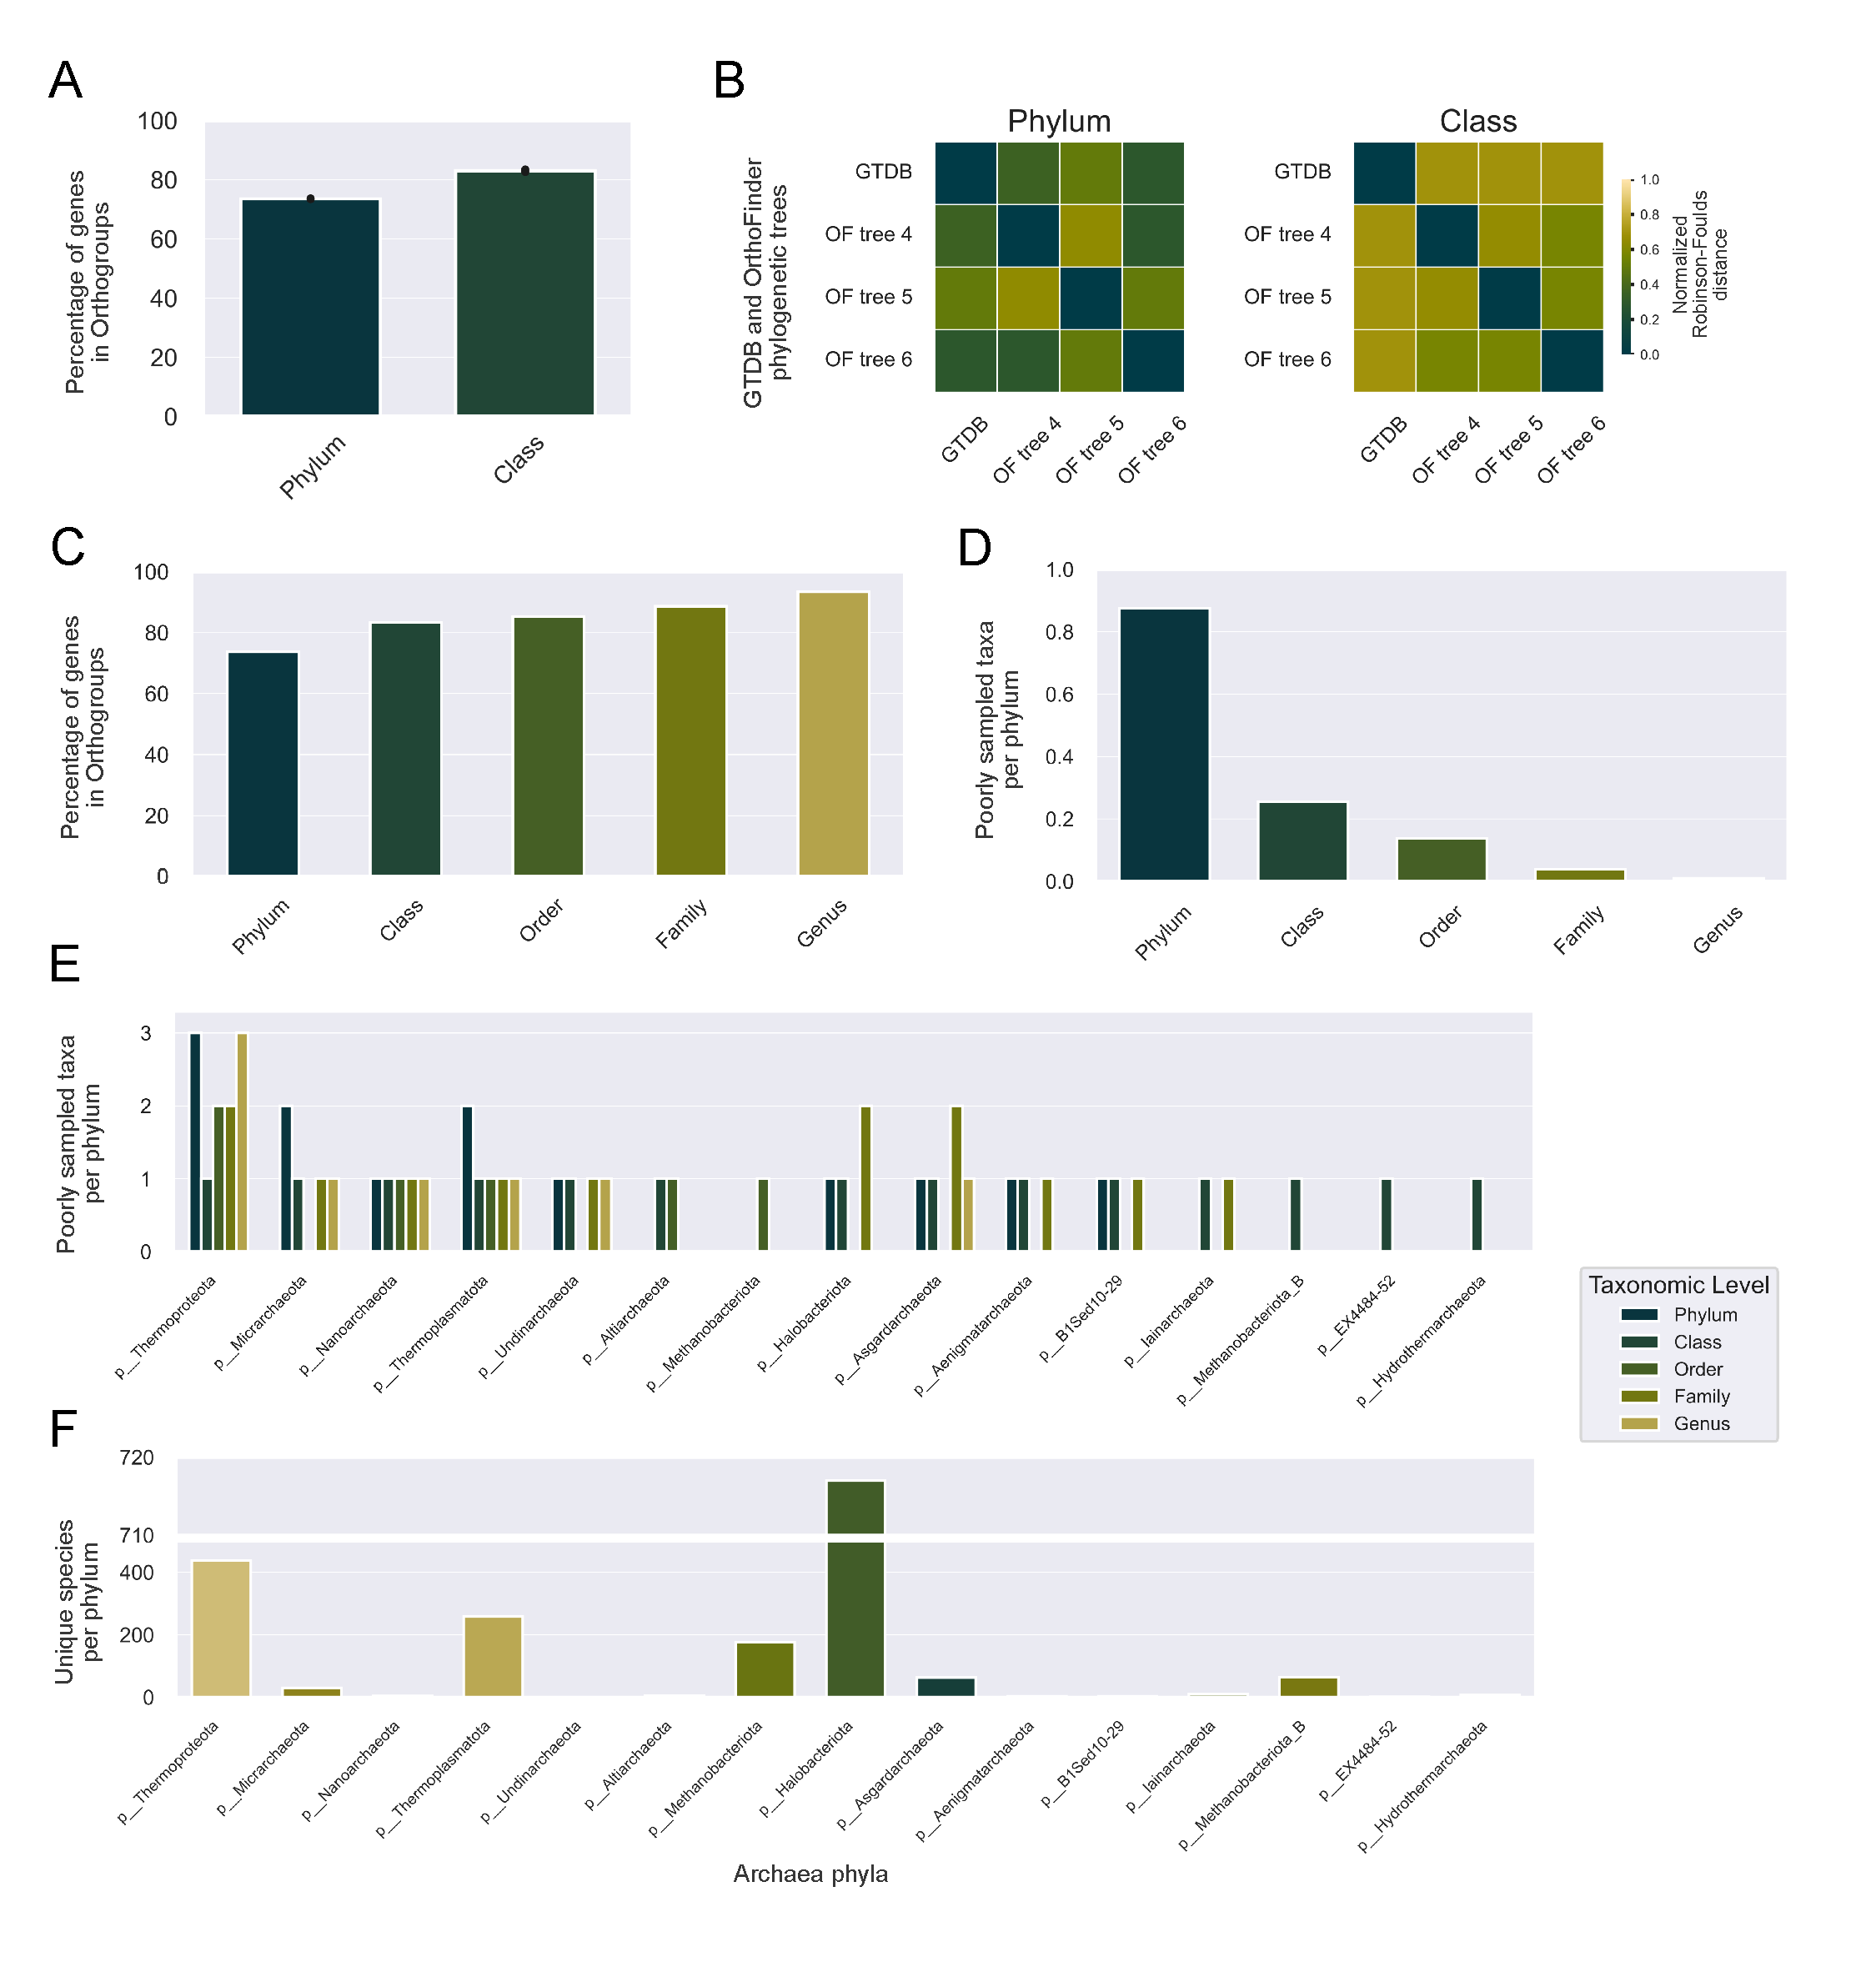
\includegraphics[width=0.97\textwidth]{fig2/fig2.pdf}
    \caption{Comparative genomics statistics of phylogenetic OrthoFinder (OF) analysis. (A) Shows the average percentage of genes assigned in orthogroups for the taxonomic levels of phylum and class for archaea. (B) Presents the Robinson-Foulds (RF) distance between the trees generated by OF as part of the aforementioned analyses, as well as their RF from the GTDB archaeal tree. (C) Compares the percentage of genes assigned in orthogroups for every archaeal taxonomic level. (D) Presents the normalized distribution of poorly sampled taxa for each taxonomic level analysis. (E) Detailed distribution of poorly sampled taxa for each taxonomic level analysis, per phylum, and (F) the number of unique species per phylum taxon.}
    \label{orthofinder_stats_figure}
\end{figure}   

A closer inspection of the statistics for individual taxa (Figure \ref{orthofinder_stats_figure}D and \ref{orthofinder_stats_figure}E) revealed that the percentage of poorly sampled genomes dropped below 5\% only at the family level (\ref{orthofinder_stats_figure}D). Interestingly, even though genomes belonging to particular phyla appear to be consistently categorized as "poorly sampled", this behavior cannot be linked to the number of species belonging to the same taxon. The Thermoproteota phylum, for example, has the highest count of "poorly sampled" species across all datasets, yet is the second richest archaeal phylum. Nanoarchaeota, on the other hand, whose genes are also consistently left out of orthogroups, comprise only of 4 species (Figure \ref{orthofinder_stats_figure}F). One has to take into account that species distribution remains uneven throughout the taxonomic levels, with some classes, orders, families, and genera that belong to the same phylum enriched more than others. Yet, with the decrease in genetic distance between species as datasets grow, and taxonomic levels become narrower, we would expect richer phyla to have a higher assignment of genes to OGs in narrower taxonomic levels.  

An initial comparison of the species trees produced by OF's STAG \cite{emms2018} and STRIDE \cite{emms2017} en-suite algorithms in Dendroscope \cite{huson2012} (found in Appendix Figures \ref{phylum_trees1} - \ref{gtdb_tree}) exposed unique tree topologies. Because of the significant missing gene orthology relationships at the phylum and class level, this did not come as a surprise. The more surprising finding came with calculating the Robinson-Foulds (RF) distance, a direct measure of phylogenetic tree similarity. RF calculates the number of nodes that are dissimilar between the phylogenetic trees under comparison, with lower values indicating a higher similarity degree. Even though the comparative genomics statistics results present the class level analyses as more-encompassing of orthology relationships, the inferred by OF species trees are more dissimilar than those for the phyla (Figure \ref{orthofinder_stats_figure}B). This could be rationalized by the fact that a smaller phylum dataset with longer genetic distances would be more likely to produce the same species tree topology. Nonetheless, it raises concerns about algorithms such as STRIDE using all genes, rather than only highly conserved ones, to infer a species tree. As Martinez-Gutierrez and Aylward \cite{martinez-gutierrez2021} have pointed out, \textit{"more genes and genomes do not necessarily improve phylogenetic accuracy"}. In light of this and considering our varying dataset sizes, we selected the GTDB domain-specific species trees for our downstream analysis.

\subsection*{Inferring ancestral genomes}
\addcontentsline{toc}{subsubsection}{Inferring ancestral genomes}

We wanted to utilize the full potential of the genomic data at hand for reconstructing ancestral metabolic networks, and avoid simplified approaches such as phylogenetic presence/absence profiles \cite{kreimer2008} or those using near-universal gene family distribution as filtering criteria \cite{xavier2021}. We therefore performed our phylogenetic analysis with OF \cite{emms2019, emms2015}, a comprehensive platform for comparative genomics that provides a standardized, accurate, fast, and scalable orthology inference approach. 

The relationship between number of each ancestor's descendants and ancestral genome size can be seen in Figure \ref{node_descendants_genomesize}. The number of descendants for node zero is a direct representation of the respective dataset size, as all descendants are utilized to infer its gene content. Leaf parents like nodes 3, 5, 10, 11, 12, 13, on the other hand, tend to have the smallest number of descendants. These relationships can be seen in the phylum-level tree topology of Figure \ref{node_descendants_genomesize} panel B. Of interest here is the uneven addition of new taxa to the various tree clades, with some clades experiencing rapid enrichment, while others remaining with few taxa. This unevenness could be a direct reflection of field sampling bias, but can be more likely be attributed to the culturability, and thus higher quality of genomic data, of specific taxa. For example, nodes 3 and 5, which represent a superphylum-level clade called DPANN, archaea with extremely small genome sizes and few cultured members \cite{dombrowski2019, dombrowski2020}, have very few descendants in all taxonomic-level datasets. What stands out the most, however, in Figure \ref{node_descendants_genomesize} panel, is the strong positive correlation between the inferred ancestral genome size and the number of descendants/initial sampling size, with a Pearson correlation coefficient close to 1 for all nodes. 

\begin{figure}[H]
    \centering
    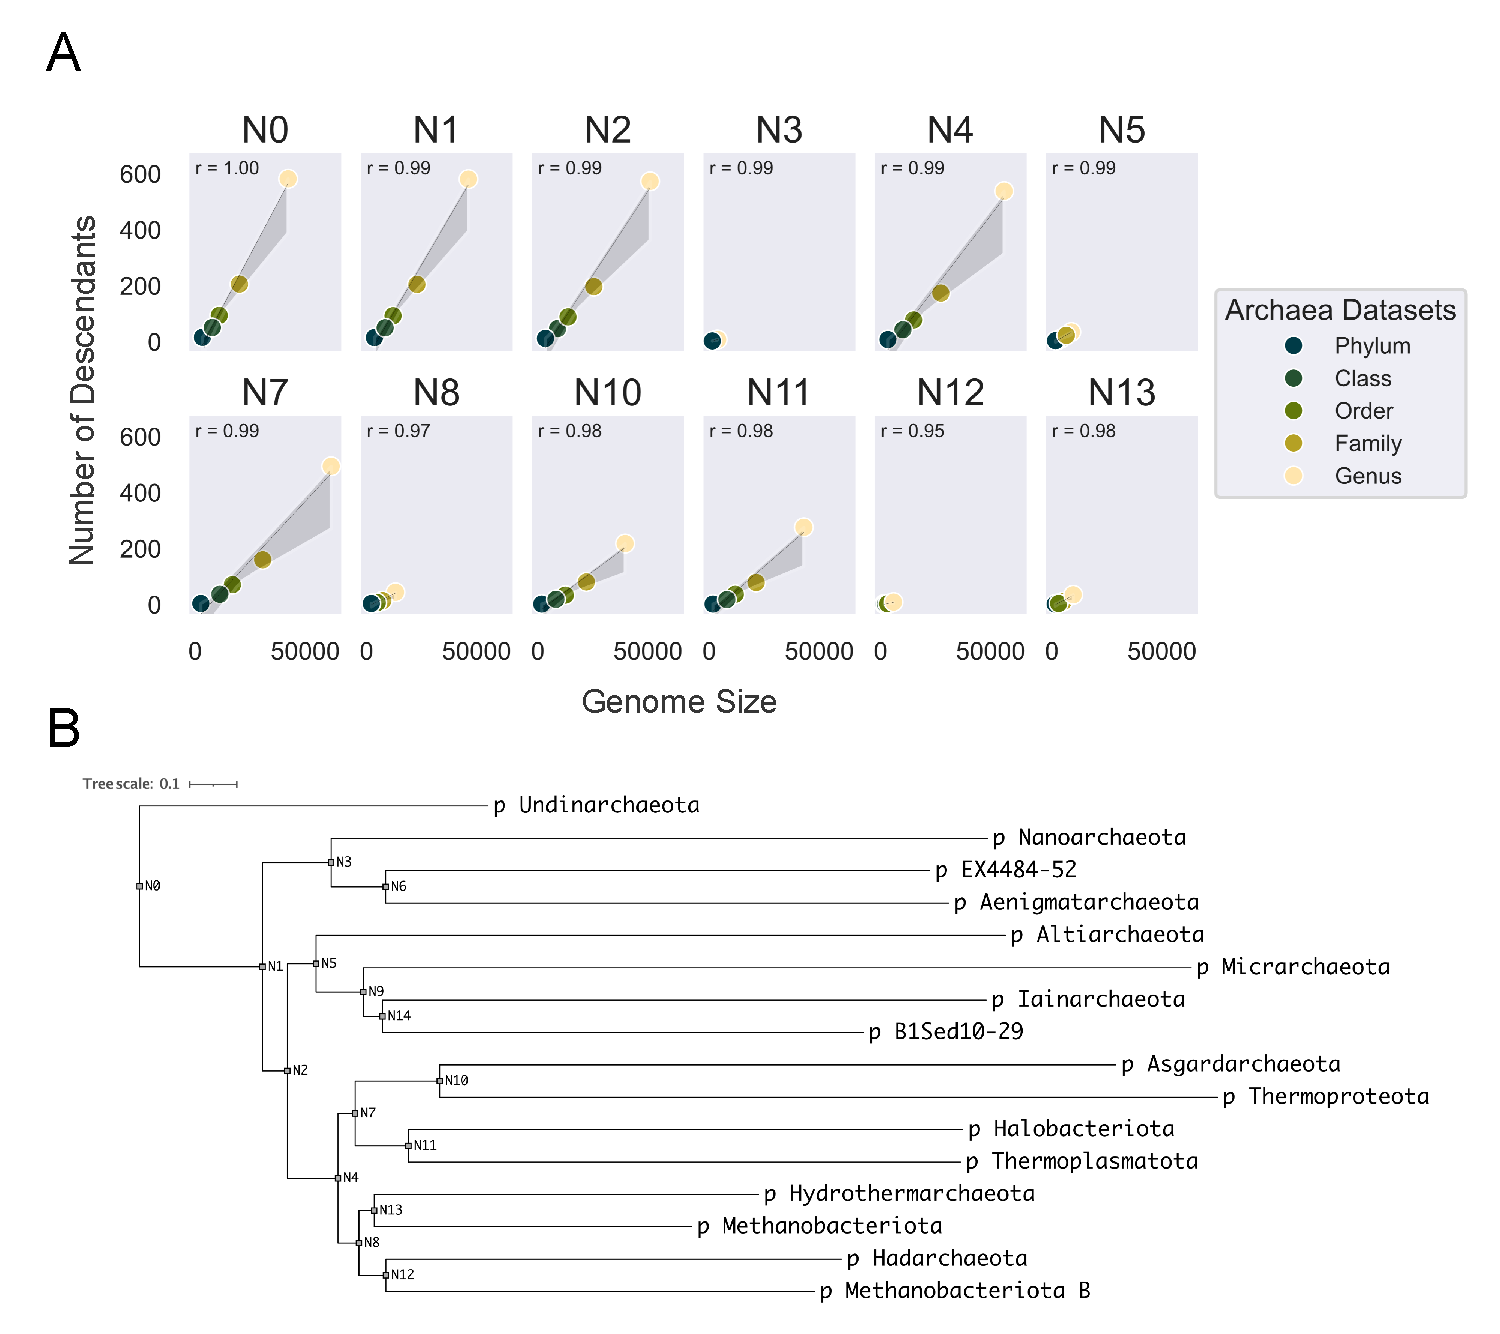
\includegraphics[width=0.95\textwidth]{fig1/fig1v2.pdf}
    \caption{Relationship between genome size and number of node descendants. (A) Shows the number of descendants of each node as a function of the inferred ancestral genome sizes, for all taxonomic levels of the archaea datasets. Colors are assigned to the five taxonomic levels, and turn lighter with narrower taxonomies. (B) Depicts the position of the nodes in the GTDB species tree, as well as their descendants. The phylum-level GTDB pruned tree has been used for simplification purposes. }
    \label{node_descendants_genomesize}
\end{figure}   


This relationship is not surprising, and can be attributed to the Duplication-Loss-Coalescence (DLC) parsimonious model for gene trees-species tree reconciliation OF utilizes. This model does not take into account horizontal gene transfer (HGT) events, and is known to overestimate gene content in ancestral genomes \cite{doolittle2003}. HGT, however, is not only omnipresent in prokaryotic evolution, but necessary for it \cite{ochman2000}. Especially when considering that any ancestral gene content reconstruction is necessarily incomplete, as the extinct gene families cannot be accounted for, it seems unreasonable that an ancient, last common ancestor would have the metabolic versatility of the entire modern biosphere. The inferred ancestral genomes of this study should therefore be considered with caution at this stage. Another model, the Duplication-Transfer-Loss (DTL) model, which accounts for HGT, is able to mitigate the tendency to infer unrealistically large ancestral genomes, getting bigger with each added genome, in the absence of HGT \cite{doolittle2003}. We therefore plan to redo our analysis by employing the DTL model, which has been shown to be more realistic and robust to gene tree uncertainty \cite{szollosi2013, szollosi2015}.

\subsection*{Ancestral Genome Functional Annotation}
\addcontentsline{toc}{subsubsection}{Ancestral Genome Functional Annotation}

For the metabolic network reconstruction of the ancestral genomes, we functionally annotated a single sequence for each of the OGs inferred to be present in the respective ancestor node. We based this decision on the rationale that an OG comprises genes that have descended from a single gene in the last common ancestor (LCA) of a group of species, and that sequences within the same OG are evolutionarily closer to each other than to sequences outside of that OG. Yet, the OGs OrthoFinder infers include both orthologs and paralogs, and functional annotation is known to be most reliable when based on orthologs, as they are expected to retain function more often than paralogs \cite{gabaldon2013a}. To assess the impact of choosing an OG representative sequence on functional annotation, we compared the functional annotations of the first sequence within each OG against the medoid sequence of the same OG (Figure \ref{waffleplot}). The medoid sequence is the sequence with the shortest genetic distance to all other sequences in the OG, and is therefore considered a better representative of the OG than the first---essentially a random---sequence. Since OF solves the gene length bias in orthogroup inference---which tends to cluster sequences of similar length together---the produced OGs include sequences of varying lengths. It may therefore be beneficial to perform a multiple sequence alignment for each OG, in the future, before choosing a representative sequence for functional annotation. Even though we do not check here for the length of the representative sequence relative to the median sequence length of an OG, there may be a selection bias towards lengths that are more common in the OG, which is also not necessarily erroneous. 

Figure \ref{waffleplot} presents the comparison statistics from the functional annotation of the two sequences belonging to the same OG in the form of a waffle plot; the dataset used for this part of the study is the phylum level archaeal one run against the Archaea (2157) eggNOG v5 database. EggNOG-mapper takes the protein sequences we provide and performs functional annotation after sequence alignment, based on the best hit. Out of 2849 OGs, for 68\% the first and medoid sequences differed, for 26\% they were the same, and 6\% were individual hits (Fig. \ref{waffleplot} orange), meaning that eggNOG-mapper found a match in the database for only one of them. Henceforth, we compare KEGG reaction and EC assignment only for different hits. Most hits do not correspond to neither a reaction ID nor EC number (Fig. \ref{waffleplot} gray blocks). Considering that the GTDB data used in our study only contain sequences predicted by Prodigal to be protein-coding, the absence of a match for the majority of the sequences is perplexing; it raises questions regarding the incompatibility between tools and databases used throughout the globe for genomic and metagenomic workflows. For hits that do find a match, 73\% share the same KEGG reaction ID, and another 71\% share the same EC number (Fig. \ref{waffleplot} purple and blue). With regard to the KEGG EC assignment, if we relax our constraints and compare EC assignments up to the third digit, which specifies the nature of the reaction \cite{mcdonald2009}, the percentage of shared EC assignments increases to 79\%. This simple statistical analysis stresses how important the choice of representative sequence is for functional annotation, even for related sequences that may have descended from the same gene. 

\begin{figure}[H]
    \centering
    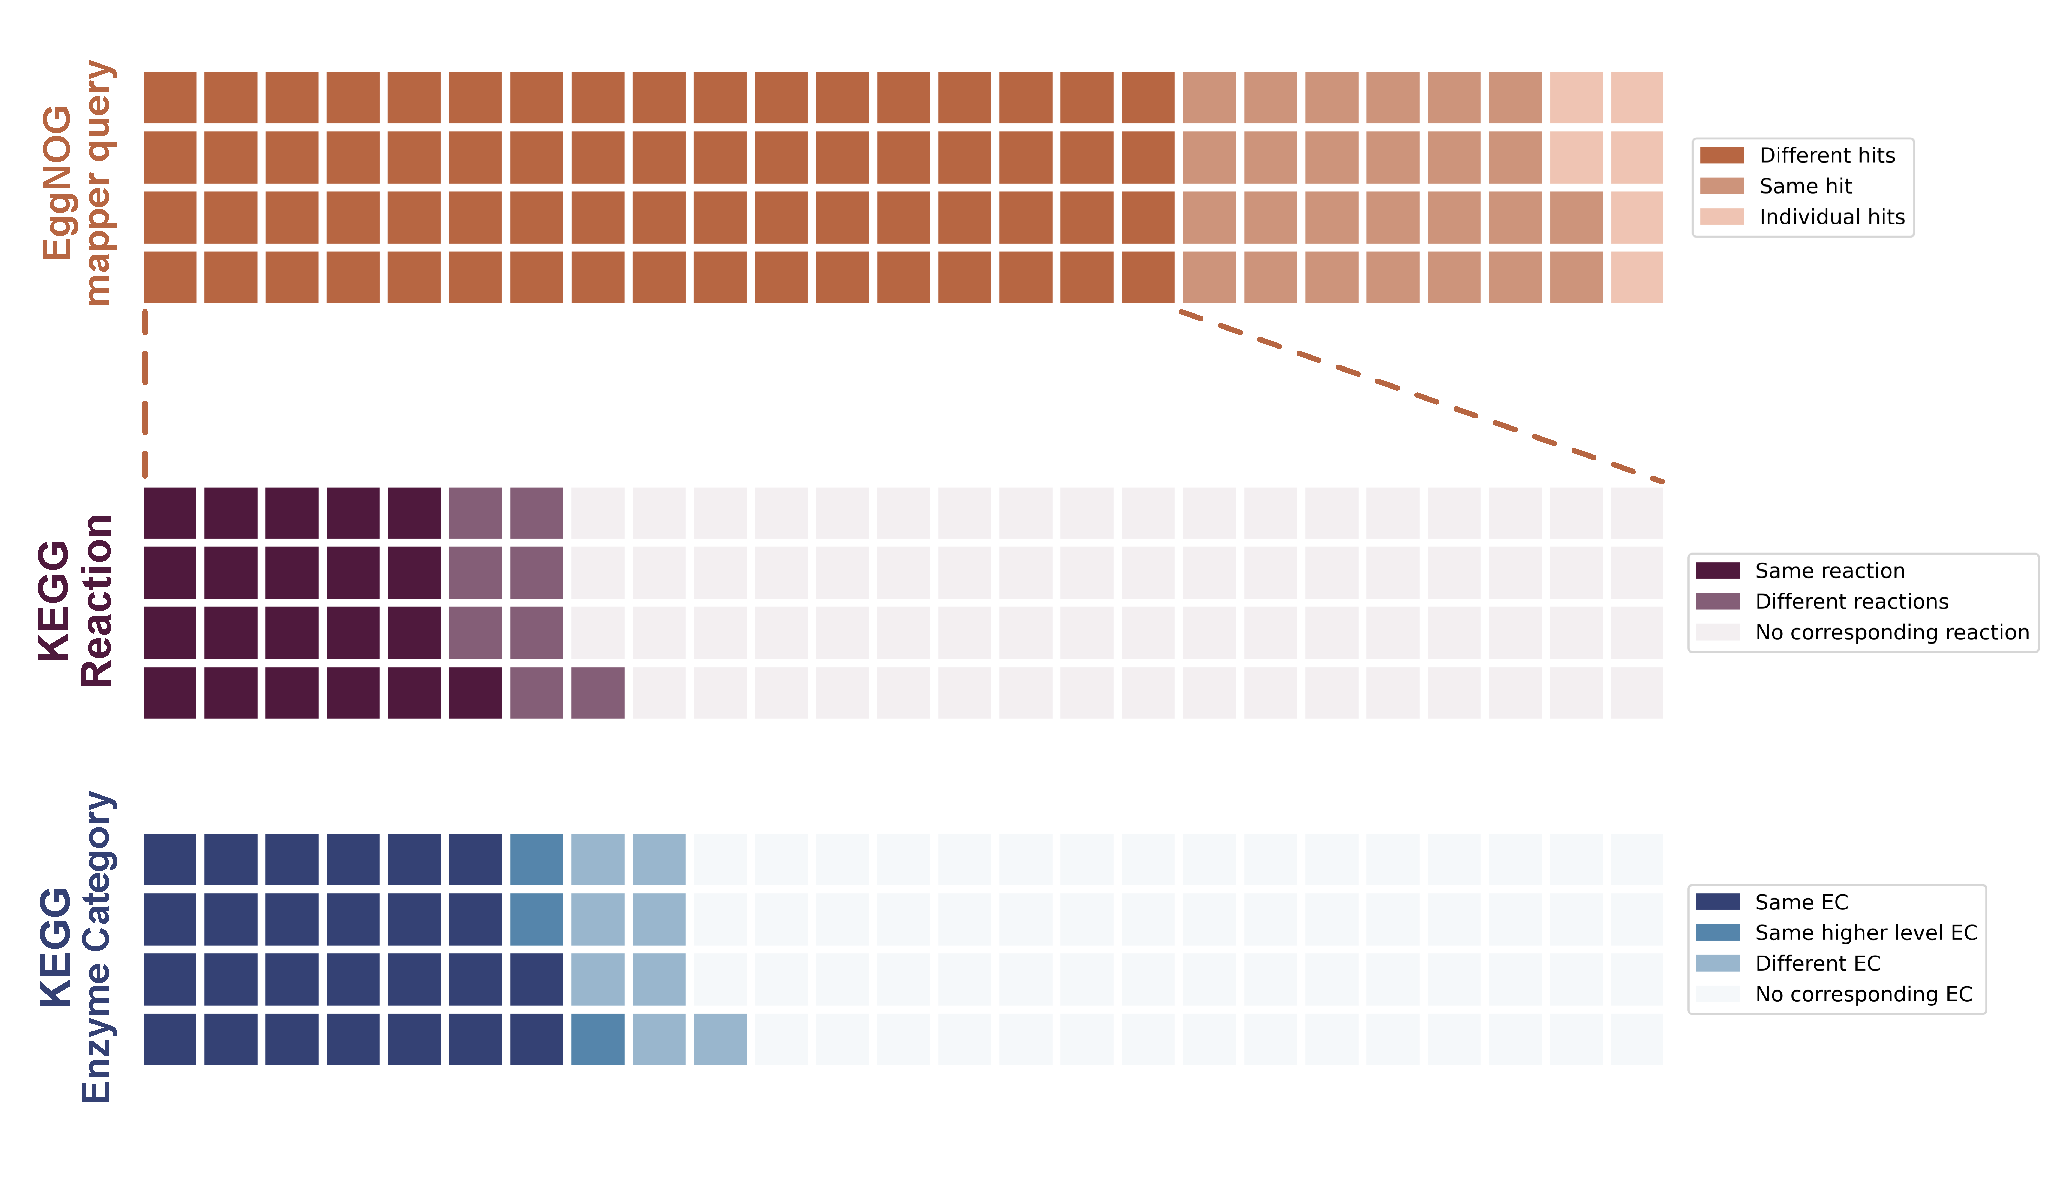
\includegraphics[width=0.95\textwidth]{waffleplot.pdf}
    \caption{Comparison of functional annotations between the first and medoid sequence of each ancestral Node zero (N0) for the archaea phylum level dataset. The waffle plot shows the percentage of a quantity---orange for number of OGs (used as a proxy for number of hits), purple for KEGG reaction number of different queries, and blue for KEGG enzyme commission (EC) number of different queries.  
     Every axis---orange, purple, and blue---shows a different statistic}
    \label{waffleplot}
\end{figure}   

For our inferred ancestral genomes belonging to the archaea phylum and class level datasets, the medoid sequence was calculated and utilized for OG functional annotation. For the rest of the datasets (found in Table \ref{datasets}), we sampled a hundred sequences from each OG at random, and calculated the medoid only for those. Since the medoid is calculated by pairwise alignment of all sequences in an OG, the computational burden increases according to the Gauss's summation formula (Equation \ref{eq:alignments}), where \textit{n} is the number of sequences. As our datasets grow in size, the number of sequences attributed to each OG increases to a point where calculating the medoid becomes extremely time-consuming. For example, an OG with 1000 sequences---which becomes common in our larger datasets---would require 500,500 pairwise alignments. We therefore opted for a computationally tractable approach, calculating the medoid for a hundred randomly sampled sequences for OGs larger than that. Instead of calculating the medoid for all OGs, we could also have annotated all sequences of an OG, and then choose the most common eggNOG OG (eggNOG orthogroup) or COG (cluster of orthologous genes) category as the representative one for the OG, as done by Xavier et al. \cite{xavier2021}. 

\begin{equation}
    \label{eq:alignments}
    \sum_{i=1}^{n} i = \frac{n(n+1)}{2}
\end{equation}

As mentioned above, the functional annotation does not only depend on the sequence itself, but on the database against which it is aligned. A feature of eggNOG-mapper version 2 \cite{cantalapiedra2021} allows for the generation of taxon-specific eggNOG databases. We therefore generated three databases spanning the prokaryotic domain, one for the Archaea (2157), one for Bacteria (2), and a general one including both domains (2157, 2). We then performed functional annotation of genes predicted to be present for certain internal tree nodes (presented in Figure \ref{node_descendants_genomesize}) against the domain-specific and the general eggNOG databases, chose for the best hit between the two runs, as described in the Methods section, and reconstructed each metabolic network based on the KEGG reaction IDs assigned by eggNOG-mapper for each best hit. Extant genomes were annotated only against the general eggNOG database. 

We also tried performing functional annotation of entire OGs, instead of single protein sequences, with profile hidden markov models (HMMs), as a more sensitive, probabilistic approach. In contrast to traditional substitution matrices, such as the BLOSUM matrix \cite{henikoff1992} we utilized to determine the medoid, profiles are position-specific scoring models and take into account specific---to each sequence---conservation patterns \cite{mount2009, gribskov1987}, and can therefore offer enhanced alignment and functional annotation quality. However, this methodology is even more time-consuming than simply calculating the medoid, and was not feasible with our current computational resources. In future analyses, we plan to use HMMs for functional annotation of the OGs, and compare the results with those obtained by the medoid method.

\subsection*{Metabolic Network Reconstruction}
\addcontentsline{toc}{subsubsection}{Metabolic Network Reconstruction}


One of the first things we noticed when mapping our inferred reaction IDs to the KEGG database was the absence of multiple IDs per dataset and often incomplete or missing fields, leading to inconsistent information between reactions; for example, some reactions include the KEGG module or pathway, while others do not. Even though the KEGG databases provide a valuable resource for the field of bioinformatics and metabolism modeling \cite{kanehisa2000}, it was primarily designed for visualization purposes, and its reactions are often unbalanced \cite{wrzodek2013} and can be even elementally inconsistent \cite{goldford2024}. For these reasons, we utilized the database compiled by Goldford et al. (2024) \cite{goldford2024}, which extends the KEGG reactions database by excluding elementally inconsistent reactions and adding detailed organic and inorganic cofactor dependencies from various other databases. 

To inspect the connectivity of the reconstructed metabolisms of putative, ancient microorganisms, we visualized the networks using iPath \cite{darzi2018}, an interactive metabolic pathway explorer that is based on four KEGG global maps. The hypothetical metabolic potential of LACA for the family-level archaea dataset can be seen in Figure \ref{fam4arc_metnet}, while the rest of LACA-inferred metabolic networks can be found in Appendix Figs. \ref{phy4arc_metnet} - \ref{gen4arc_metnet}. Even at the phylum-level, the network seems relatively well-connected, with isolated reactions being dispersed across the entire map. The smallest of the reconstructed metabolic networks, after all, contains 1192 reactions. 

\begin{figure}[H]
    \centering
    \includegraphics[width=0.98\textwidth]{metabolism/fam_arc_N0.pdf}
    \caption{Reconstruction of LACA's metabolic network from extant life, for the family-level archaea dataset. In black: enzymes and metabolic pathways that were inferred to be present in LACA.}    
    \label{fam4arc_metnet}
\end{figure}

%Another drawback of using KEGG Orthology (KOs), instead of COGs---which correspond to wider gene families---\cite{tatusov2003}, to construct hypothetical metabolism models of ancient microorganisms, is that gene families that were likely present in those organisms are divided into multiple KO families that appear in particular taxonomic groups and may only be inferred for younger ancestors \cite{moody2024}.

Phylogenetic-based metabolic network reconstruction enables the mapping of genetic information to genome distance from the tree root. We aimed to explore the emergence and evolution of individual ECs across the tree of life, a topic that has not been previously investigated. For this, we acquired the distance of all nodes from the tree root and used it as a proxy for evolution. All enzyme categories are present in the reconstructed LACA metabolism (Figure \ref{ec_vs_rootdist_fam}B). The relative abundance of ligases and oxidoreductases is higher in the inferred ancient metabolisms, while that of transferases declines. Lyases and isomerases are universally more limited and do not become enriched over time. This divergence may indicate a different rate of innovation for various ECs or suggest that specific types of enzymes are more prone to either loss or gain.

No other significant differences or patterns are observable, so it may be beneficial to divide the tree into multiple clades and track EC evolution within specific groups of species rather than across the entire tree. This approach will be especially important if we increase the deep branch resolution by reconstructing the metabolic networks of all possible internal tree nodes. Even though the relative abundance of the six EC categories varies between inferred and extant microorganisms, their distribution across the tree follows a similar pattern, reflecting the species distribution across the tree (Fig. \ref{ec_vs_rootdist_fam}A). Small variations, such as the increase in transferases at a distance of around 1.5 from the tree root, may indicate an enrichment of this enzyme category in certain species, possibly due to specialization or an evolutionary advantage.

\begin{figure}[H]
    \centering
    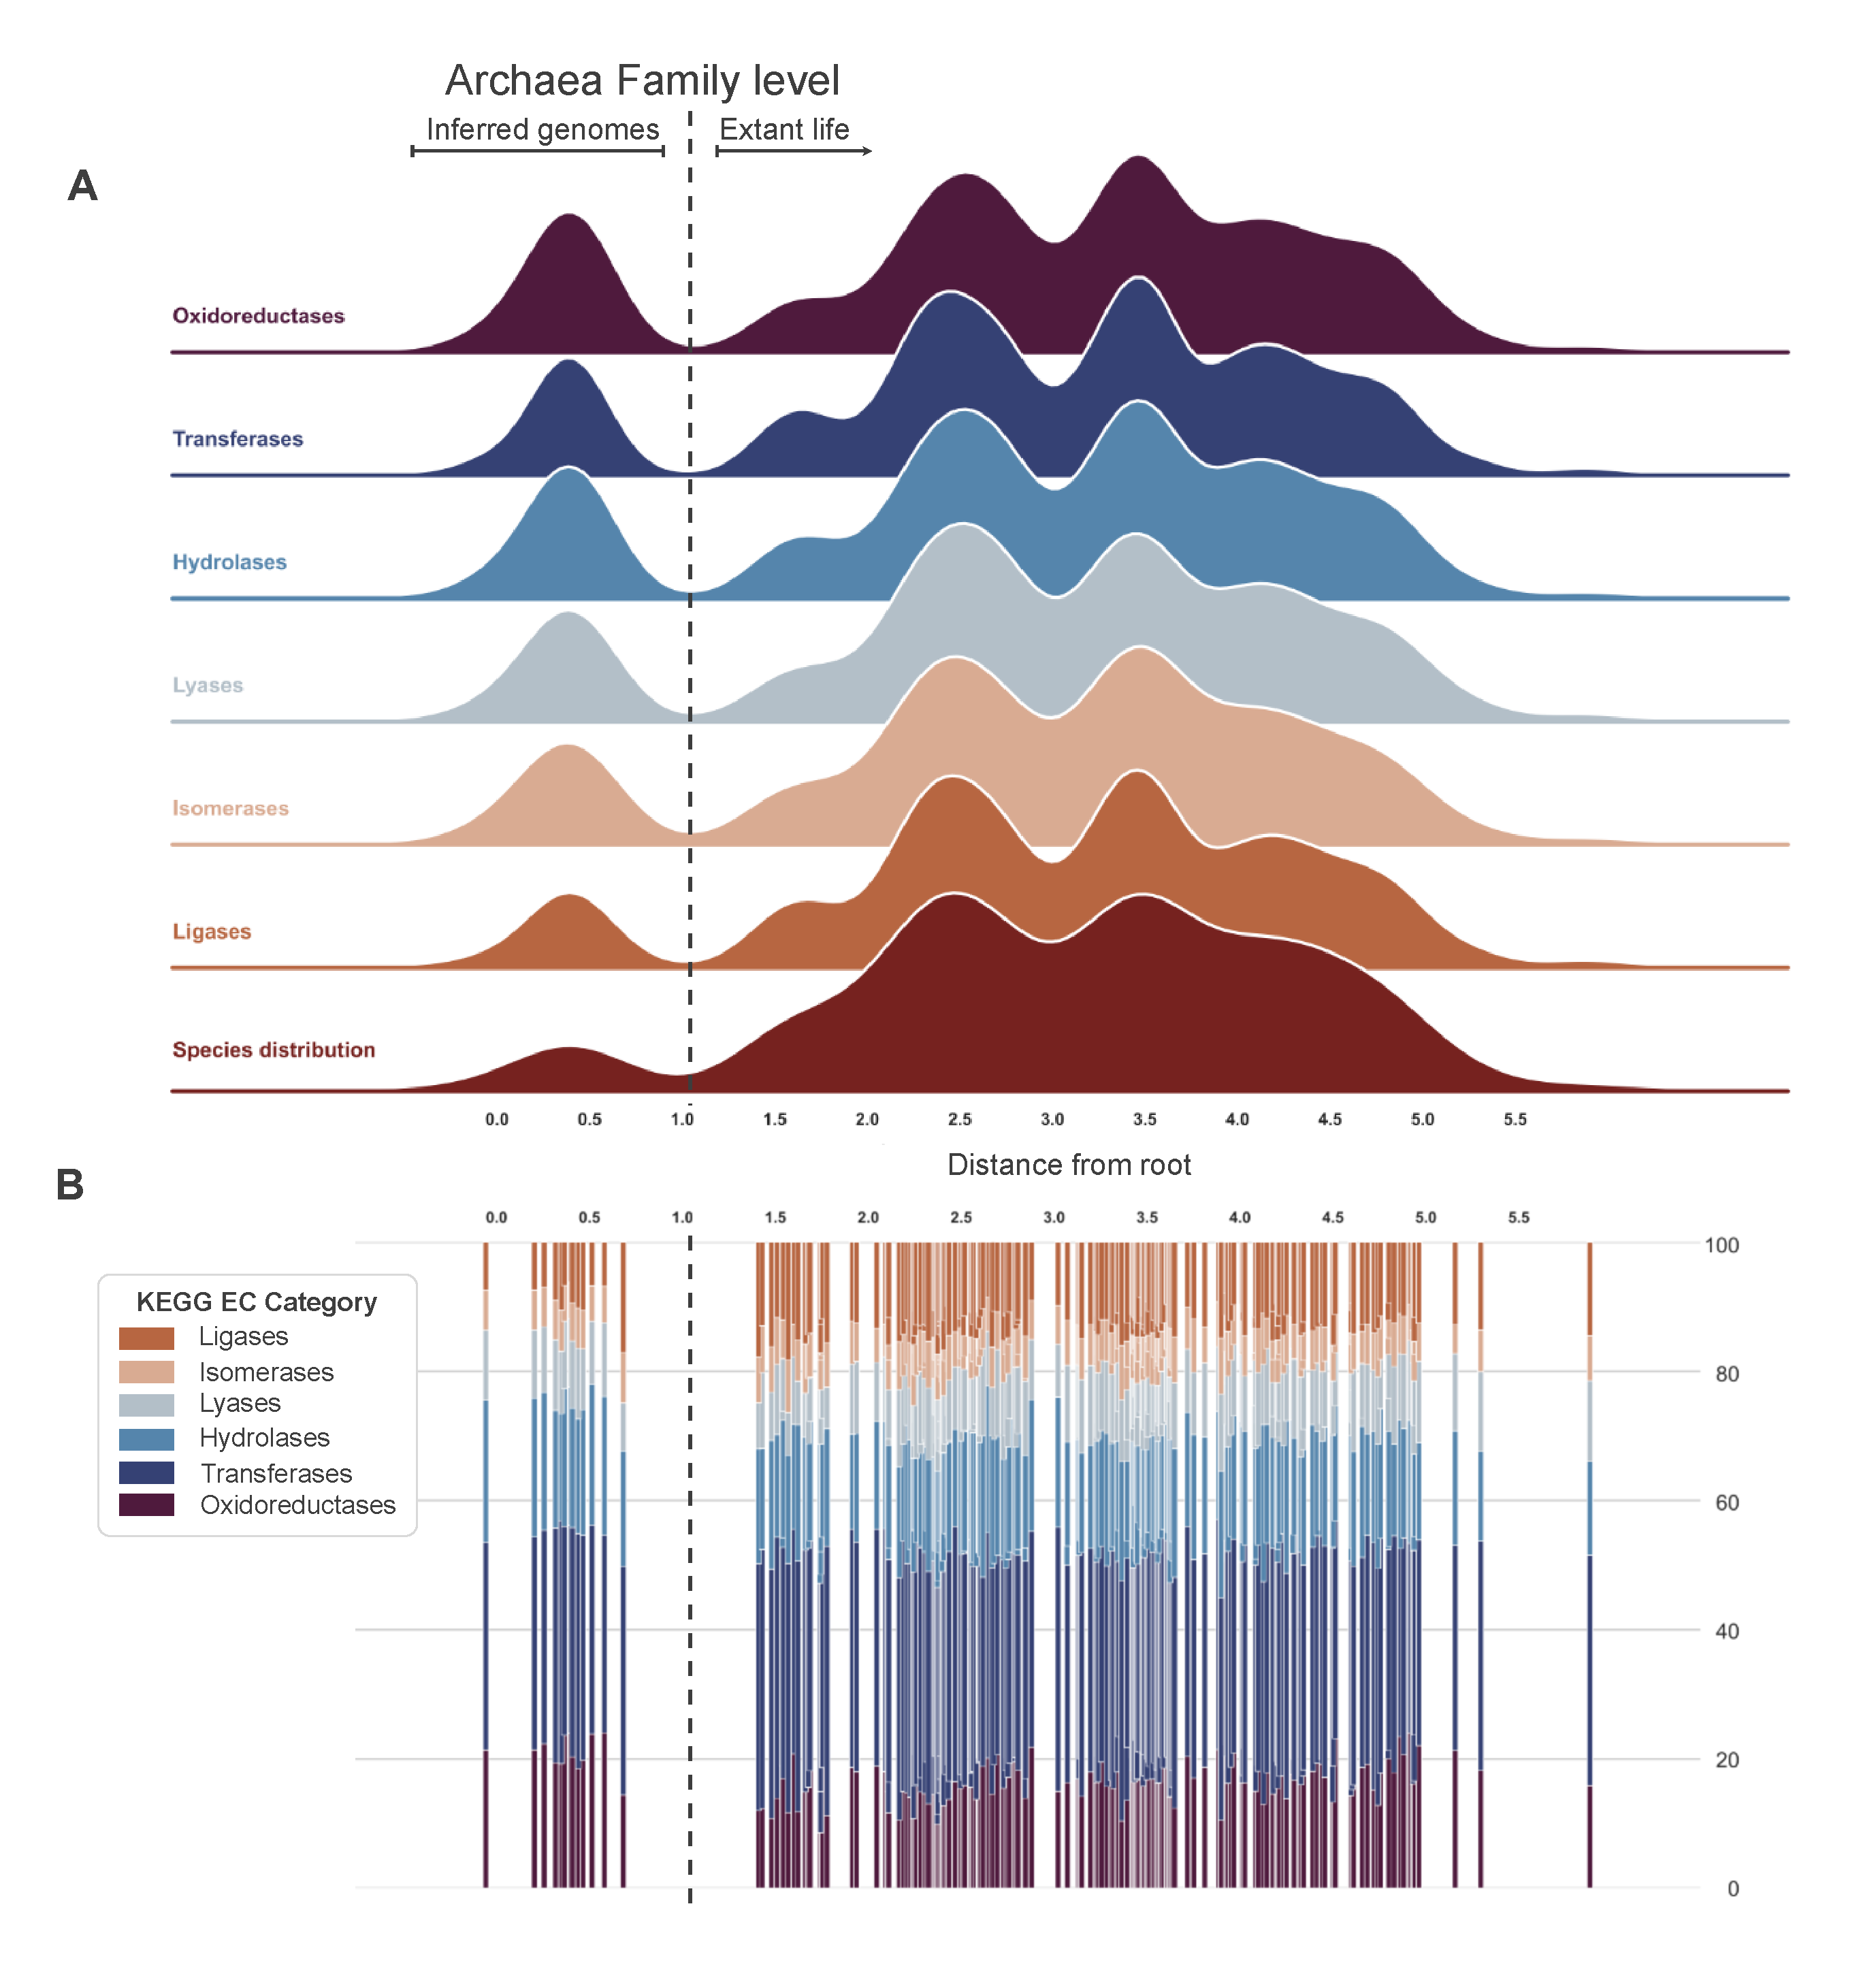
\includegraphics[width=0.9\textwidth]{ridgeplots/ec_vs_rootdist_fam.pdf}
    \caption{Evolution of individual enzyme categories for the family-level archaea dataset. The dashed line separates the inferred ancient metabolisms, on the left, from the extant ones, on the right. The ridgeplot of panel (A) displays the distribution of each category as a function of distance from the tree root, with the last axis presenting the species distribution. (B) shows the relative abundance of each category at that particular distance as a stacked barplot.}
    \label{ec_vs_rootdist_fam}
\end{figure}  

\subsection*{Metabolic Network Expansion}
\addcontentsline{toc}{subsubsection}{Metabolic Network Expansion}

** gray covers the reactions of the expanded network. They always will be less populated than the black ones. The blue dots (scope) include the red dots (seed set).

\begin{figure}[H]
    \centering
    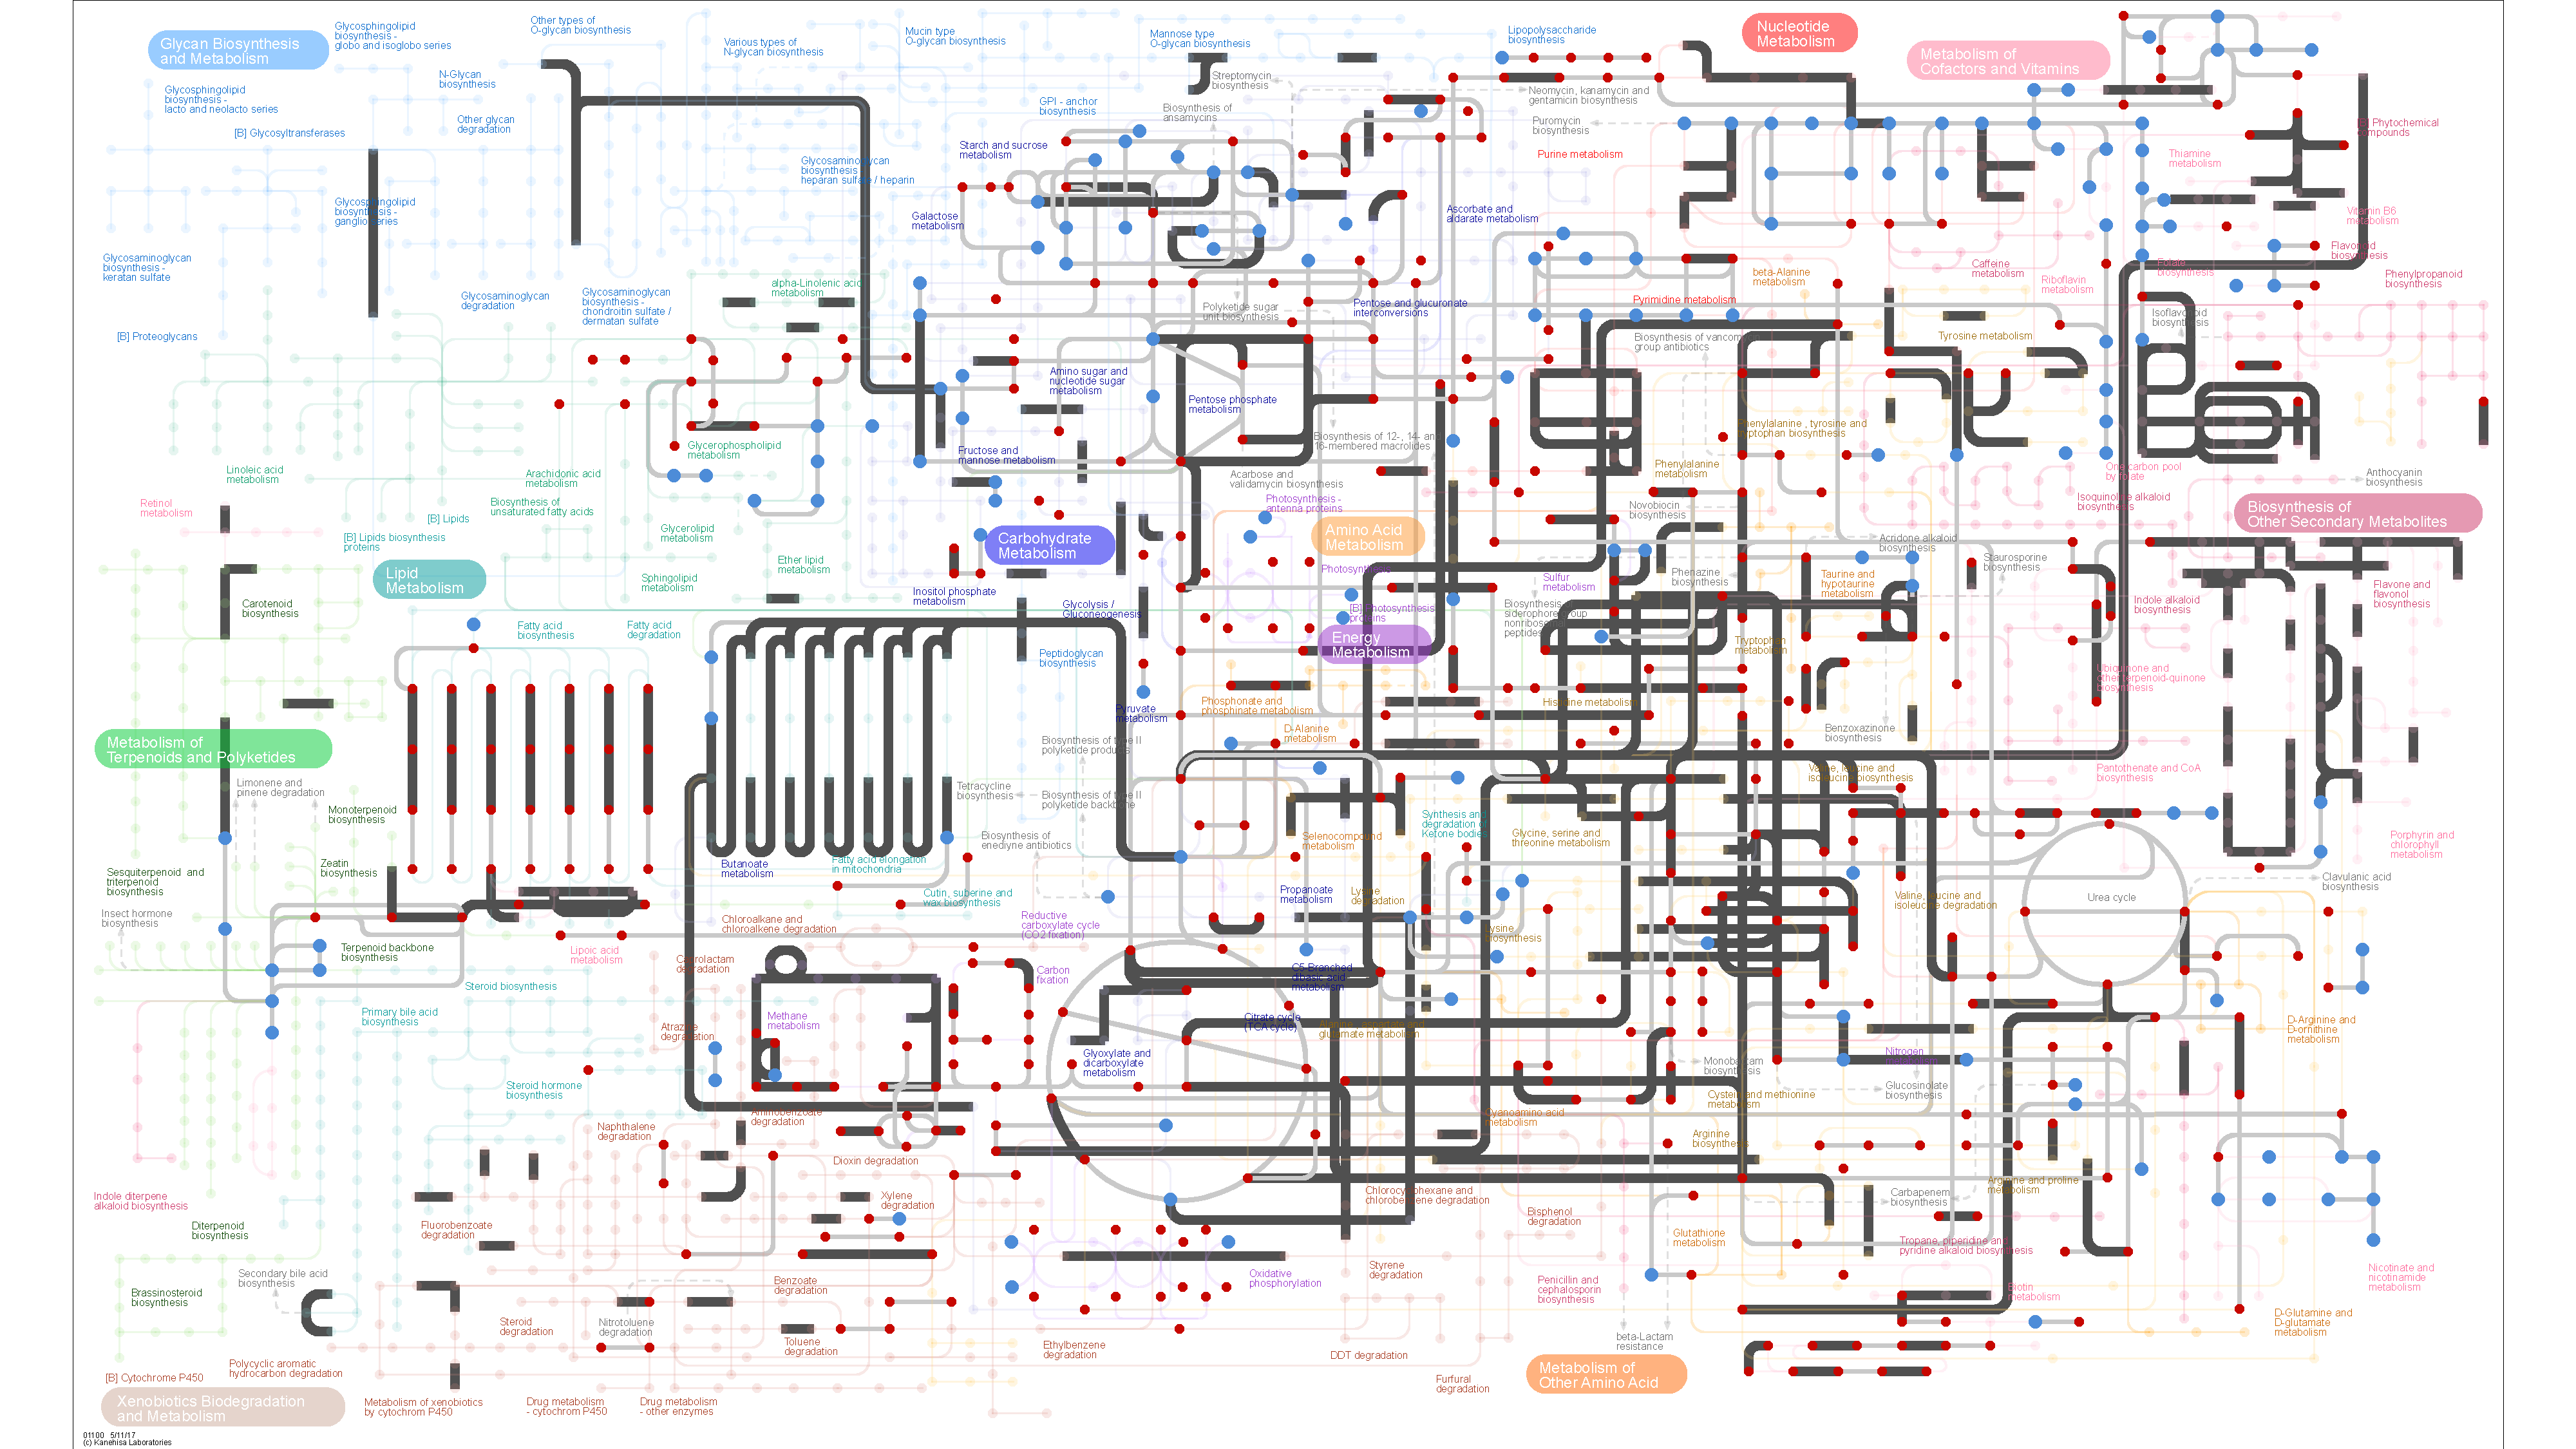
\includegraphics[width=0.98\textwidth]{metabolism/fam_N0_exp.pdf}
    \caption{Reconstruction of LACA's metabolic network from extant life, for the family-level archaea dataset. In black: enzymes and metabolic pathways that were inferred to be present in LACA. In gray: enzymes and metabolic pathways of the expanded network. Red dots: seed set compounds present in the reconstructed network. Blue dots: scope compounds after network expansion.}    
    \label{fam4arc_metnetexp}
\end{figure}

\begin{figure}[H]
    \centering
    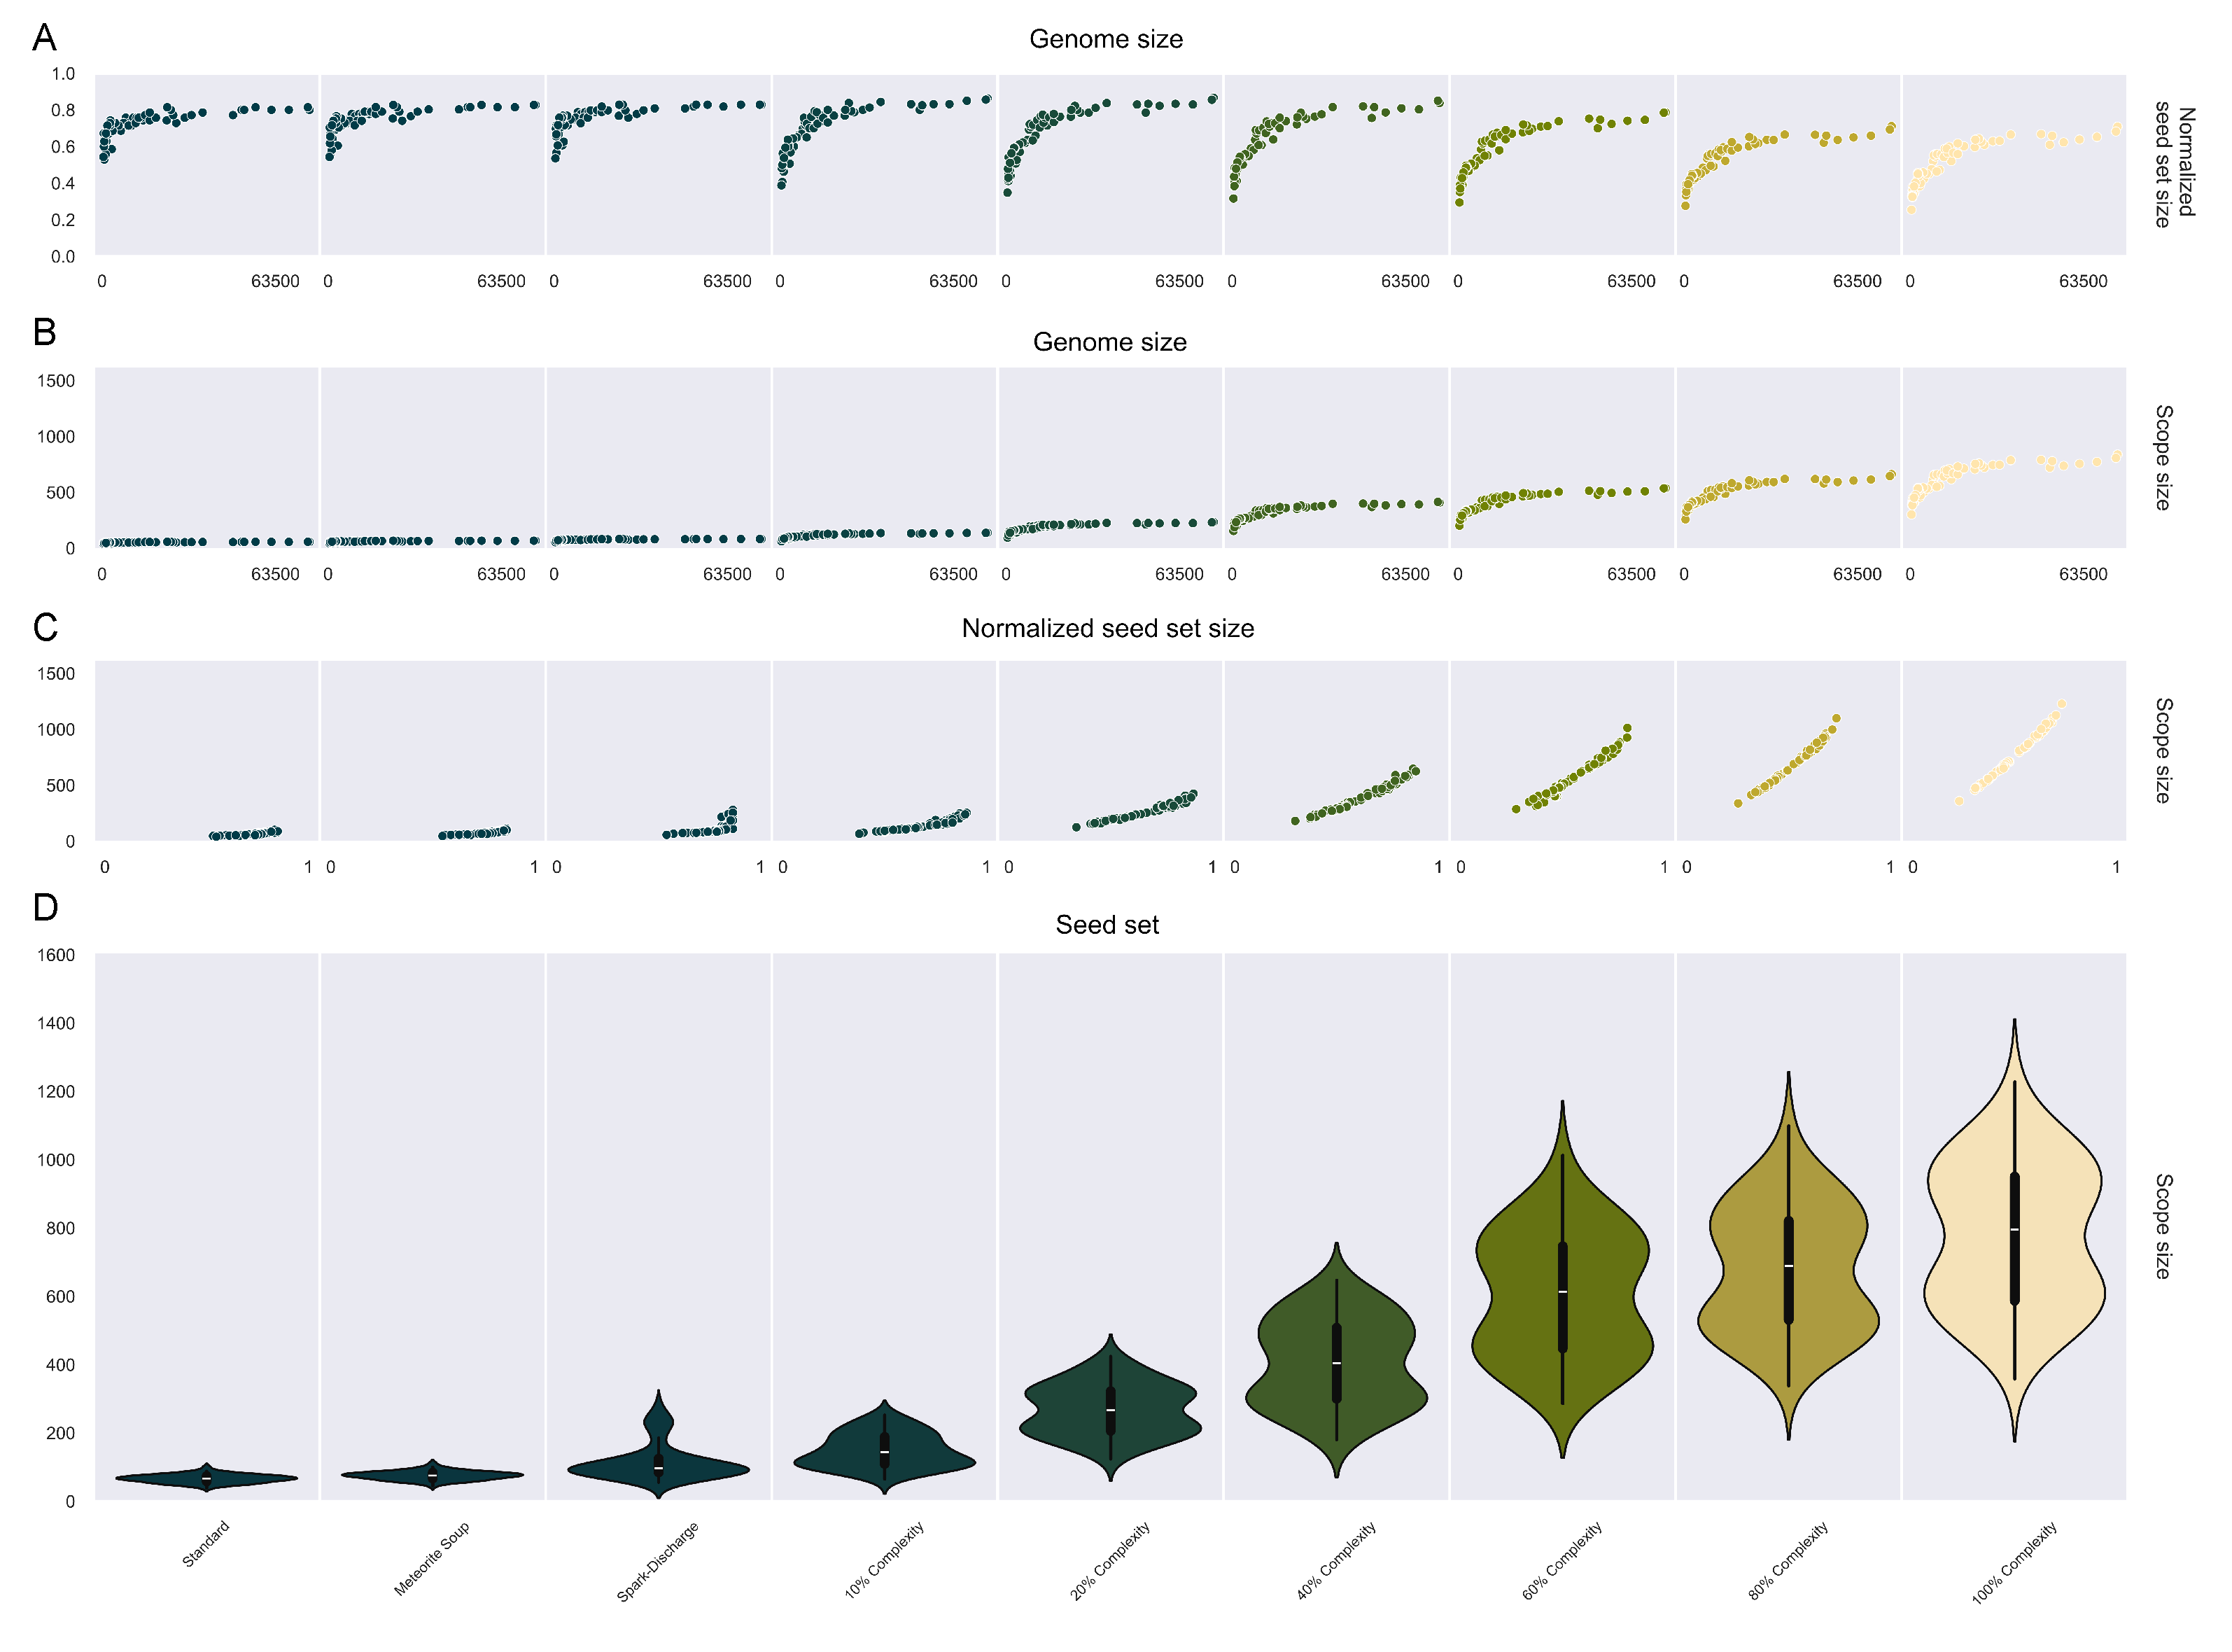
\includegraphics[width=0.98\textwidth]{overview_expansion/overview_ancient_final.pdf}
    \caption{}
    \label{overview_ancient}
\end{figure}   


\begin{figure}[H]
    \centering
    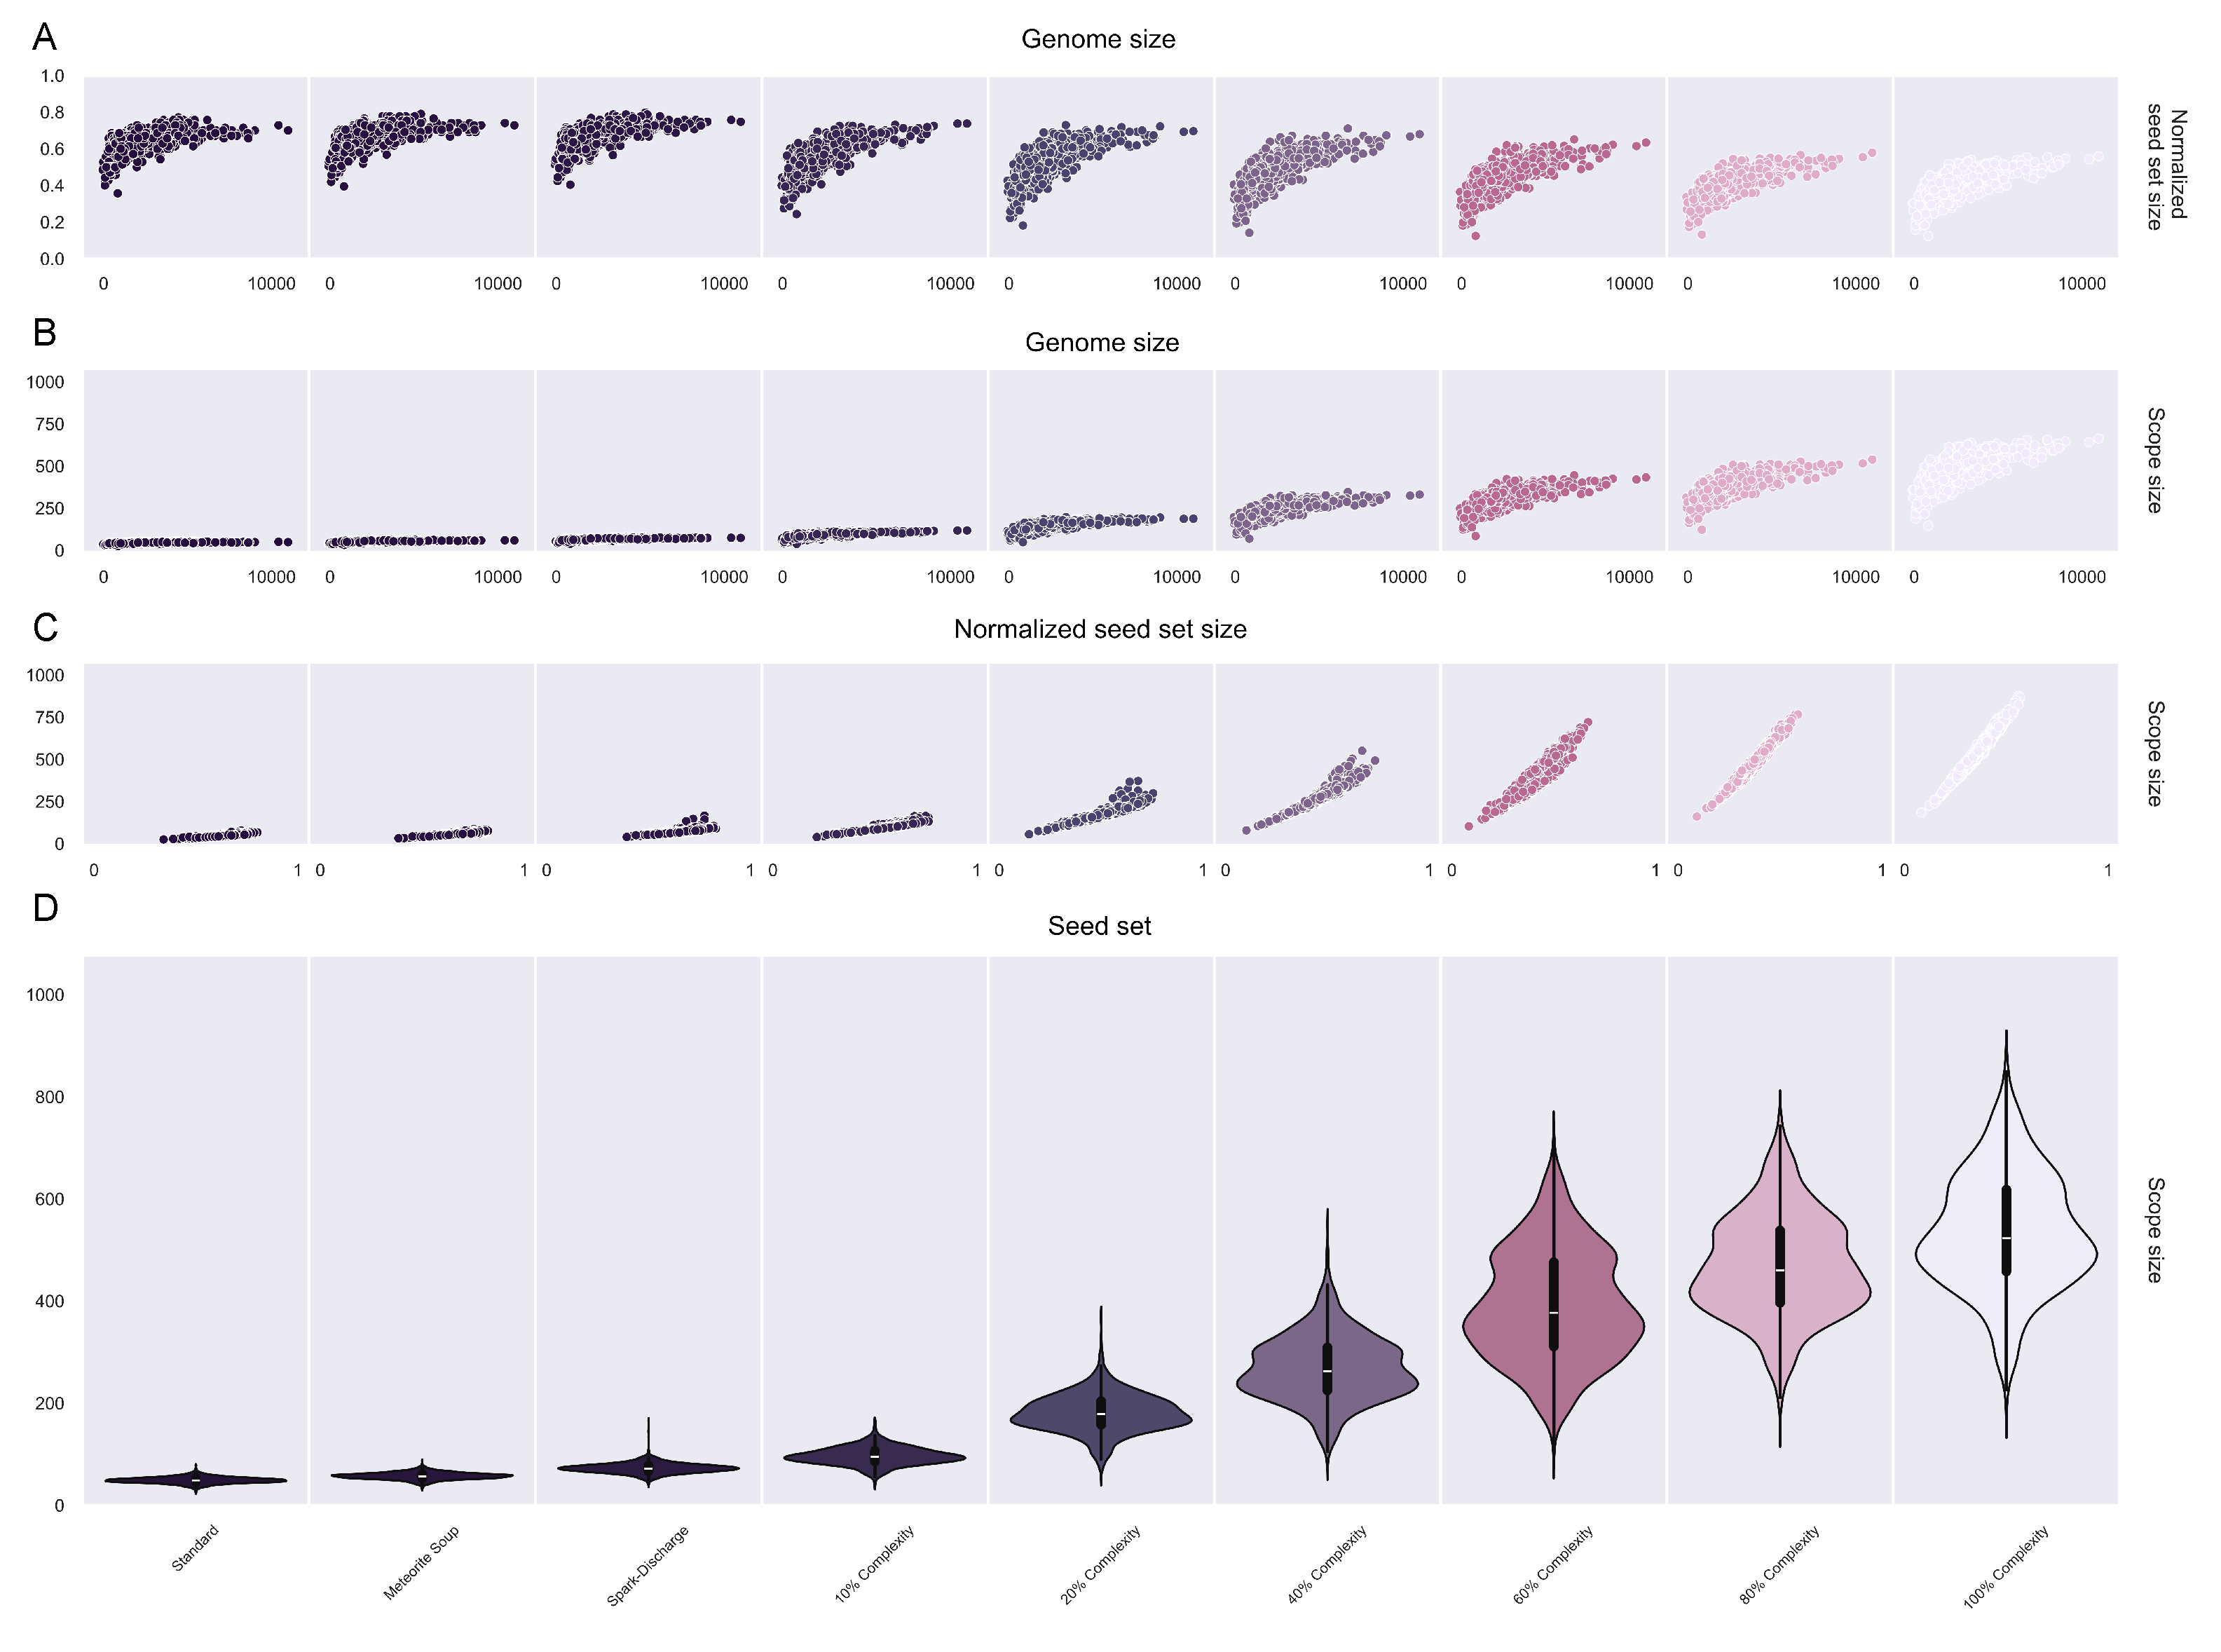
\includegraphics[width=0.98\textwidth]{overview_expansion/overview_extant_final.pdf}
    \caption{}
    \label{overview_extant}
\end{figure}   

\begin{figure}[H]
    \centering
    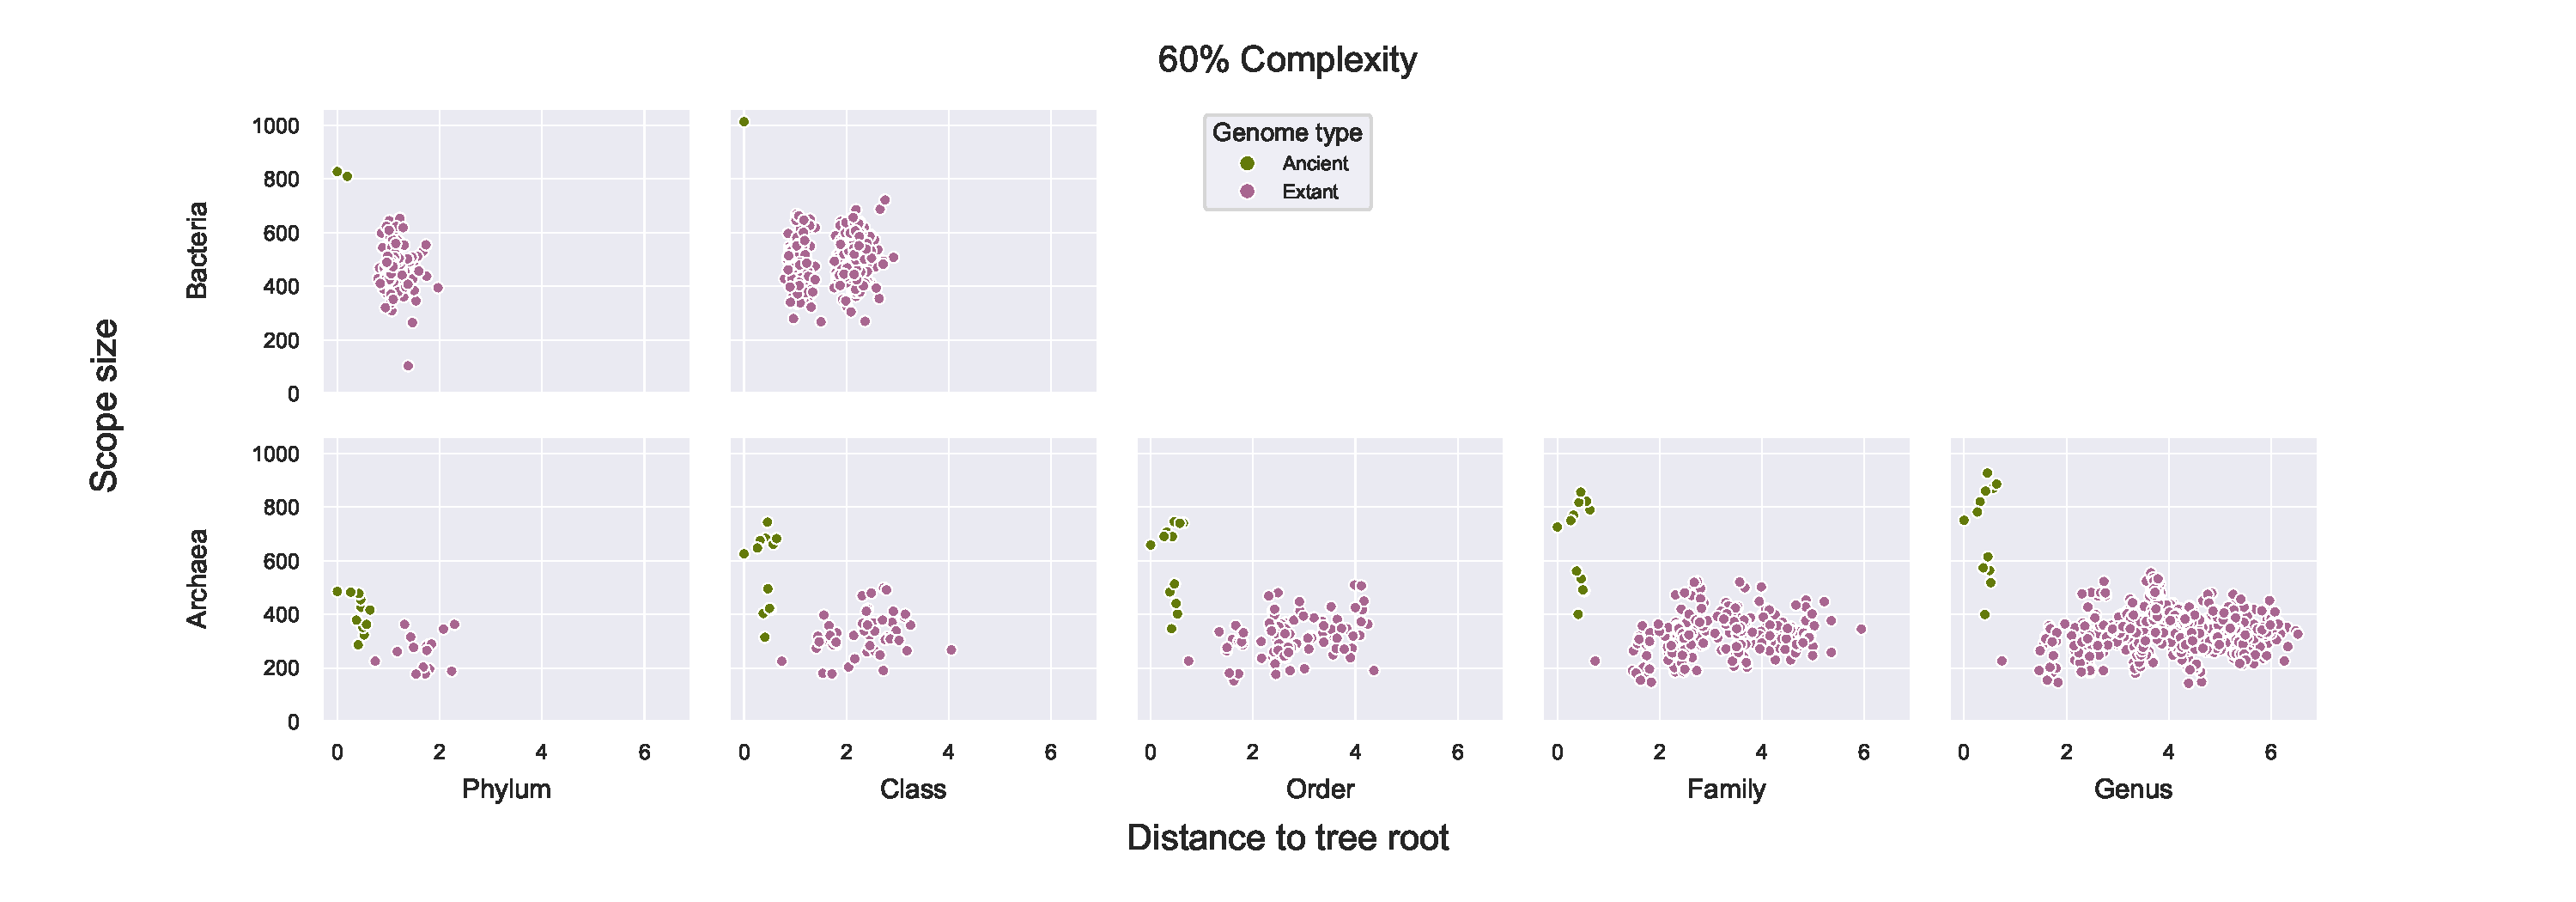
\includegraphics[width=0.95\textwidth]{scopesize_vs_disttoroot/0.6_ss_rootdist.pdf}
    \caption{}
    \label{0.6_scopesize}
\end{figure}   

\begin{figure}[H]
    \centering
    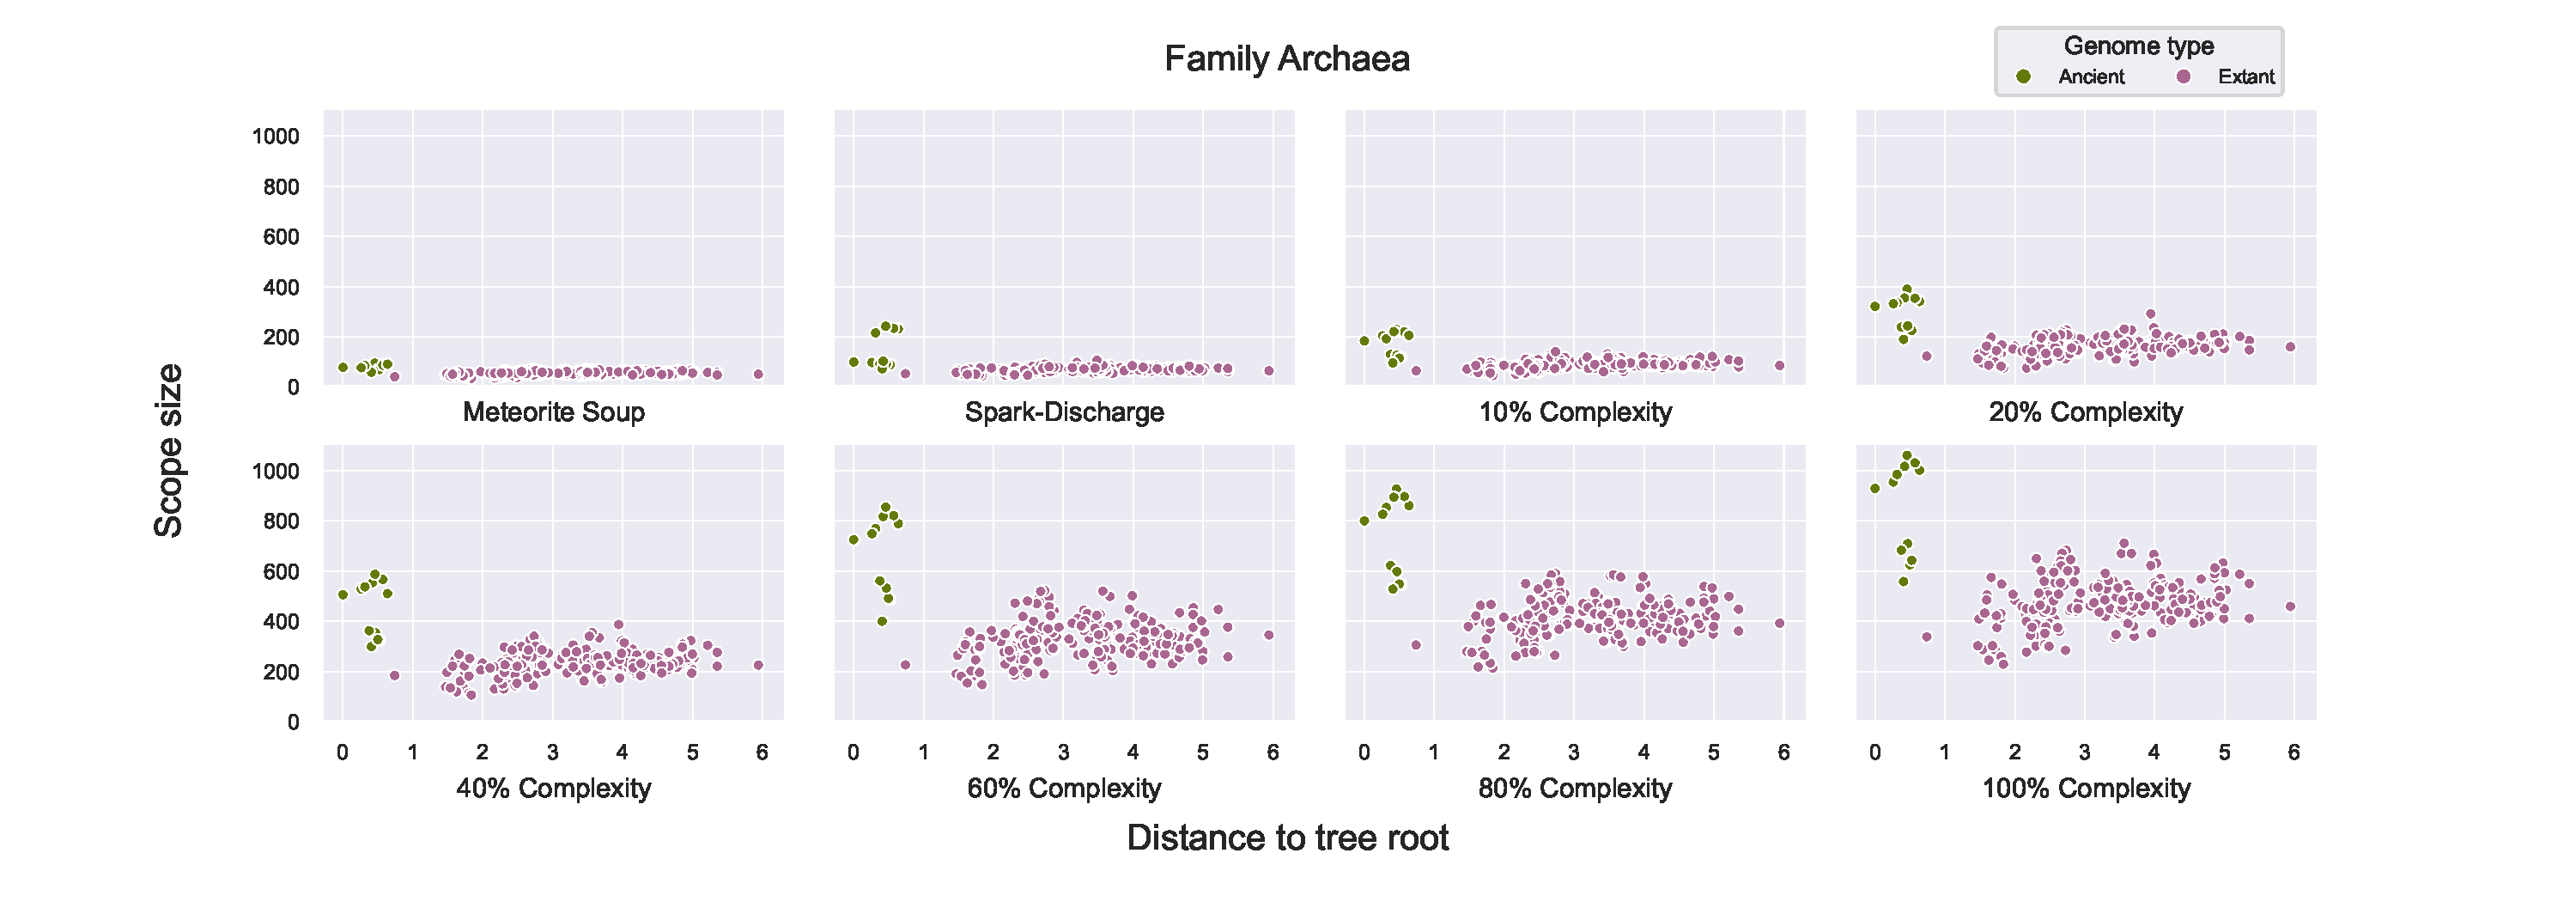
\includegraphics[width=0.95\textwidth]{scopesize_vs_disttoroot/fam4arc_ss_rootdist.pdf}
    \caption{}
    \label{fam_scopesize}
\end{figure}   



\begin{itemize}
    \item For inferred ancient genomes. Explaining main figure.
        \item Network patchiness (not all seeds being present in network, view iterations, low expansion)
        \item Maybe a figure to present patchiness of an N0 network? See how well seeds are "represented" there 
    \item Additional figure: EC values vs root distance (how it changes)
    \item For extant genomes. Explaining main figure.
\end{itemize}
%\section{Conclusions \& Outlook}
\normalsize

This research project is the first to explore the expansion of metabolic networks constrained by phylogenetic relationships, and to investigate the effect of taxon sampling on ancient genome inference. 

Phylogenetic analyses appear robust to random taxon sampling for the same dataset size. While including more species can better capture the evolutionary relationships between genes and gene families, it does not necessarily enhance species tree accuracy, as previously stated \cite{martinez-gutierrez2021}. These results suggest that depending on the research question, the inclusion of more species may be beneficial. For instance, studies aiming to define Archaeal or Bacterial Tree topologies will benefit from more limited taxon sampling, while studies like this one need broader sampling to capture the full extent of prokaryotic diversity. 

Results can vary significantly depending on both taxon sampling and the evolutionary model used for ancient gene content inference. Unlike previous research, which has investigated the physiology and metabolic potential of prokaryotic ancestors such as LUCA, LACA, and LBCA, we have employed a different parsimonious evolutionary model, the DCL model. This model does not account for horizontal gene transfer, which is integral to prokaryotic life. Consequently, the inferred genome sizes correlate positively with the number of species included in the analysis, with ancient gene content being multiple times larger than the average extant genome for any given dataset of the analysis. The DCL model, however, remains relevant. By shifting focus from the hypothesis that a single microorganism gave rise to all extant diversity to the possibility that a pool of microorganisms from the ancient biosphere evolved into modern life, the DCL model can provide valuable insights into the core metabolic functions of extant life.

Regarding the reconstruction of both extant and ancient metabolic networks using eggNOG-mapper, a gold standard and state-of-the-art tool for gene functional annotation, we found that a portion of annotated genes expected to be assigned a KEGG function were not assigned one. This finding underscores two points of interest in bioinformatics research: the discrepancy of gene family clustering algorithms and function assignment (KOs, COGs, eggNOGs) between the various tools and databases used in genomic and metagenomic workflows, and the need for transitioning to a more comprehensive database than KEGG for metabolic modeling. 

As far as the evolution of metabolism is concerned, conclusions are less concrete. The current analysis points to the existence of all six enzyme categories in the ancient biosphere. Their relative abundance, however, was probably different to that of extant life.

Performing metabolic network expansion with various seed sets across the extant and extinct parts of the tree of life challenges the previously held view that this process reflects evolution-like traits. We show that the expansion solely depends on the nature, topology, and number of seeds used for expansion, and echos the flow of chemical information within the network. Different seeds will yield differentially expanded networks, which highlights the importance of nutrient availability for proper metabolic function. 

The future of this research project is full of exciting possibilities. An important development is the creation of a \textit{'poor species detection'} algorithm. This tool will automate the identification of genetically underrepresented species in a dataset and enable the gradual integration of new closely-related taxa. The aim is to improve initially poor taxon sampling over time, while keeping the dataset size minimal, making the process both time- and cost-effective. This approach may also estimate under-sampled species in the tree of life, facilitating future sampling efforts.

Another potential improvement lies in the evolutionary analysis of metabolism we have performed. Instead of analyzing EC evolution across the tree of life, it will be more informative to focus on enzyme evolution within specific clades. This approach will allow for a more detailed understanding of the evolution of metabolic pathways for specific groups of microorganisms with specialized metabolisms, such as methanogens, halophiles, or thermophiles.

The current study has only scratched the surface of what is possible with regard to metabolic network expansion. A very useful extension of the analysis would be to use MNE to quantify a system's metabolic potential based on metabolite availability in the environment, essentially by developing a metric to measure expansion. Since our current, randomly generated seed sets are sometimes poorly integrated into the reconstructed metabolic networks, it would be beneficial to create manually curated seed sets of comparable size and complexity. This would allow for a more detailed investigation of the flow of chemical information within specific networks of interest. 

The most valuable addition to the MNE analysis would be integrating the minimal seed set approach. This method would help identify the nutritional requirements of putative ancient microorganisms and provide insights into the environmental conditions they may have inhabited.

Despite its exploratory nature, this project provides valuable insights into the challenges of modern phylogenetics and introduces a new perspective on the nature of MNE. Overall, these observations underscore the importance of delving deeper into the data, questioning it, and maintaining an open mind when investigating the deepest branches of the tree of life.

\section{References}

\printbibliography[heading=none]

\newpage
\appendix
\section{Appendix}
\counterwithin{figure}{section}
\setcounter{figure}{0}
\counterwithin{table}{section}
\setcounter{table}{0}
\noappendixindent

\subsection*{A1. Phylogenetic Analysis}
\normalsize
All shown phylogenetic trees have been visualized with Dendroscope \cite{huson2012}.

\begin{figure}[h!tbp]
    \centering
    \renewcommand{\thefigure}{A\arabic{figure}}
    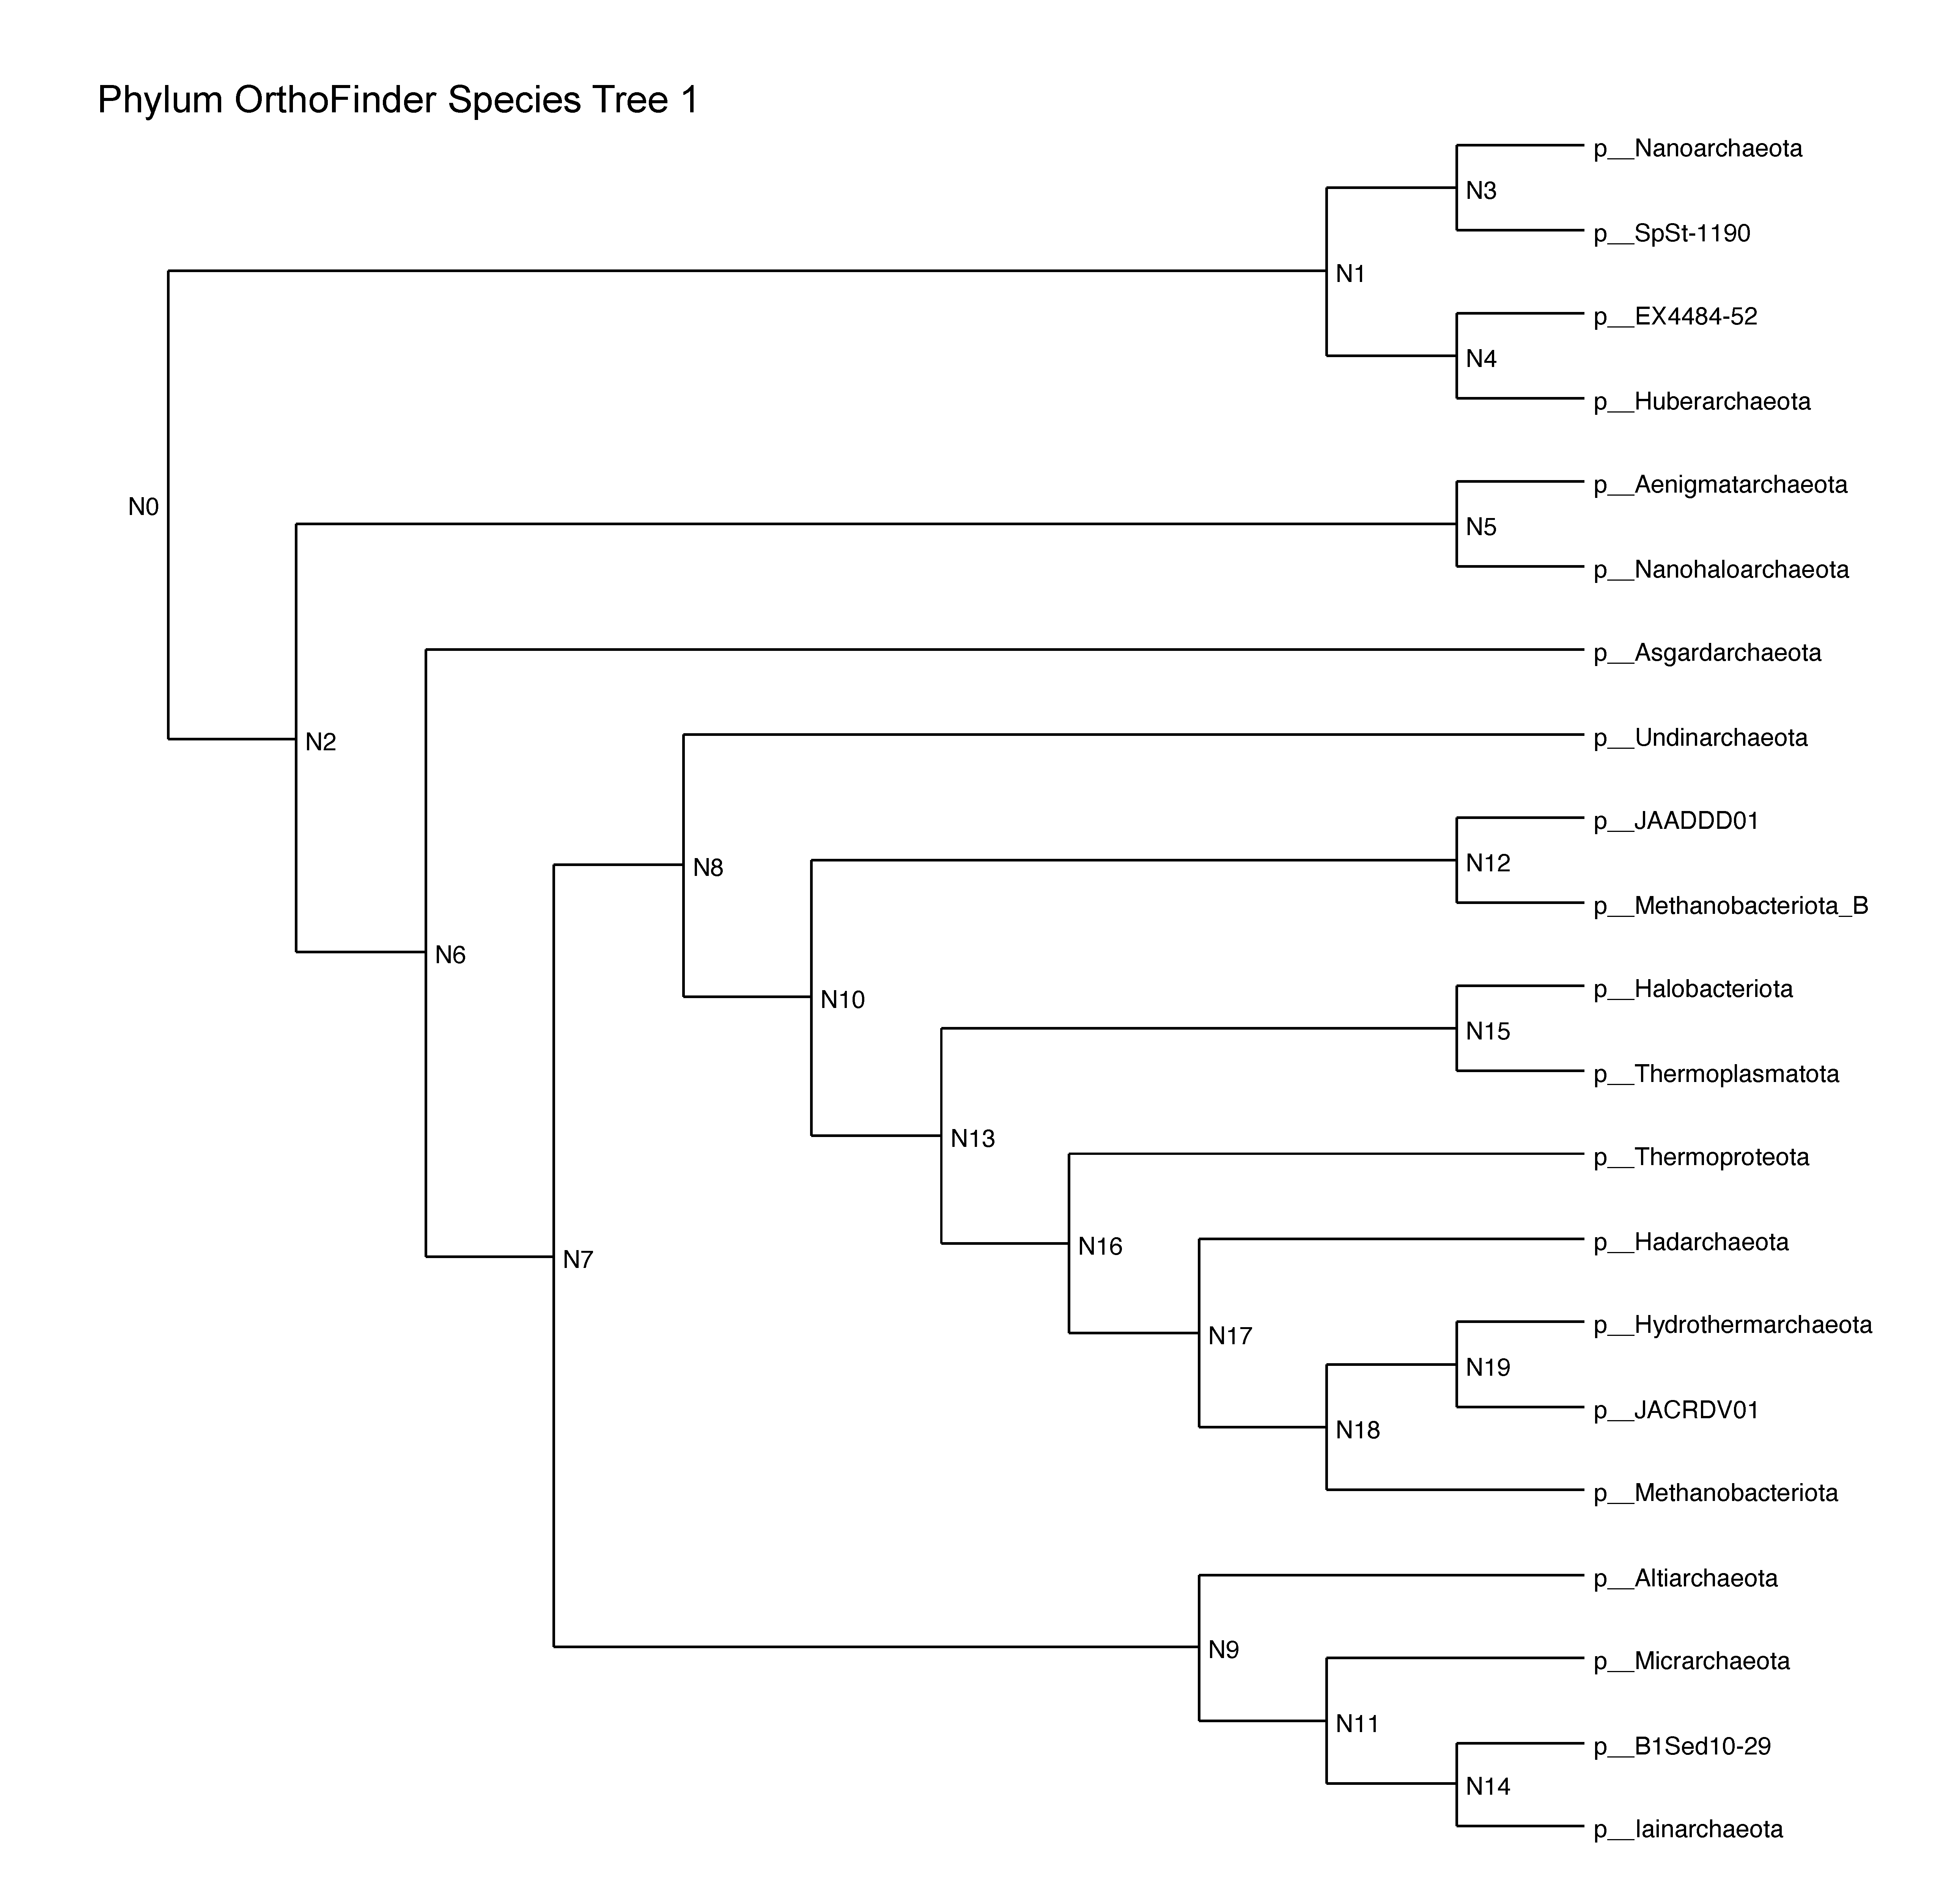
\includegraphics[width=0.5\textwidth]{trees/phy1arc}
    \caption{OrthoFinder-inferred species tree; first analysis.}
    \label{phylum_trees1}
\end{figure}

\begin{figure}[h!tbp]
    \centering
    \renewcommand{\thefigure}{A\arabic{figure}}
    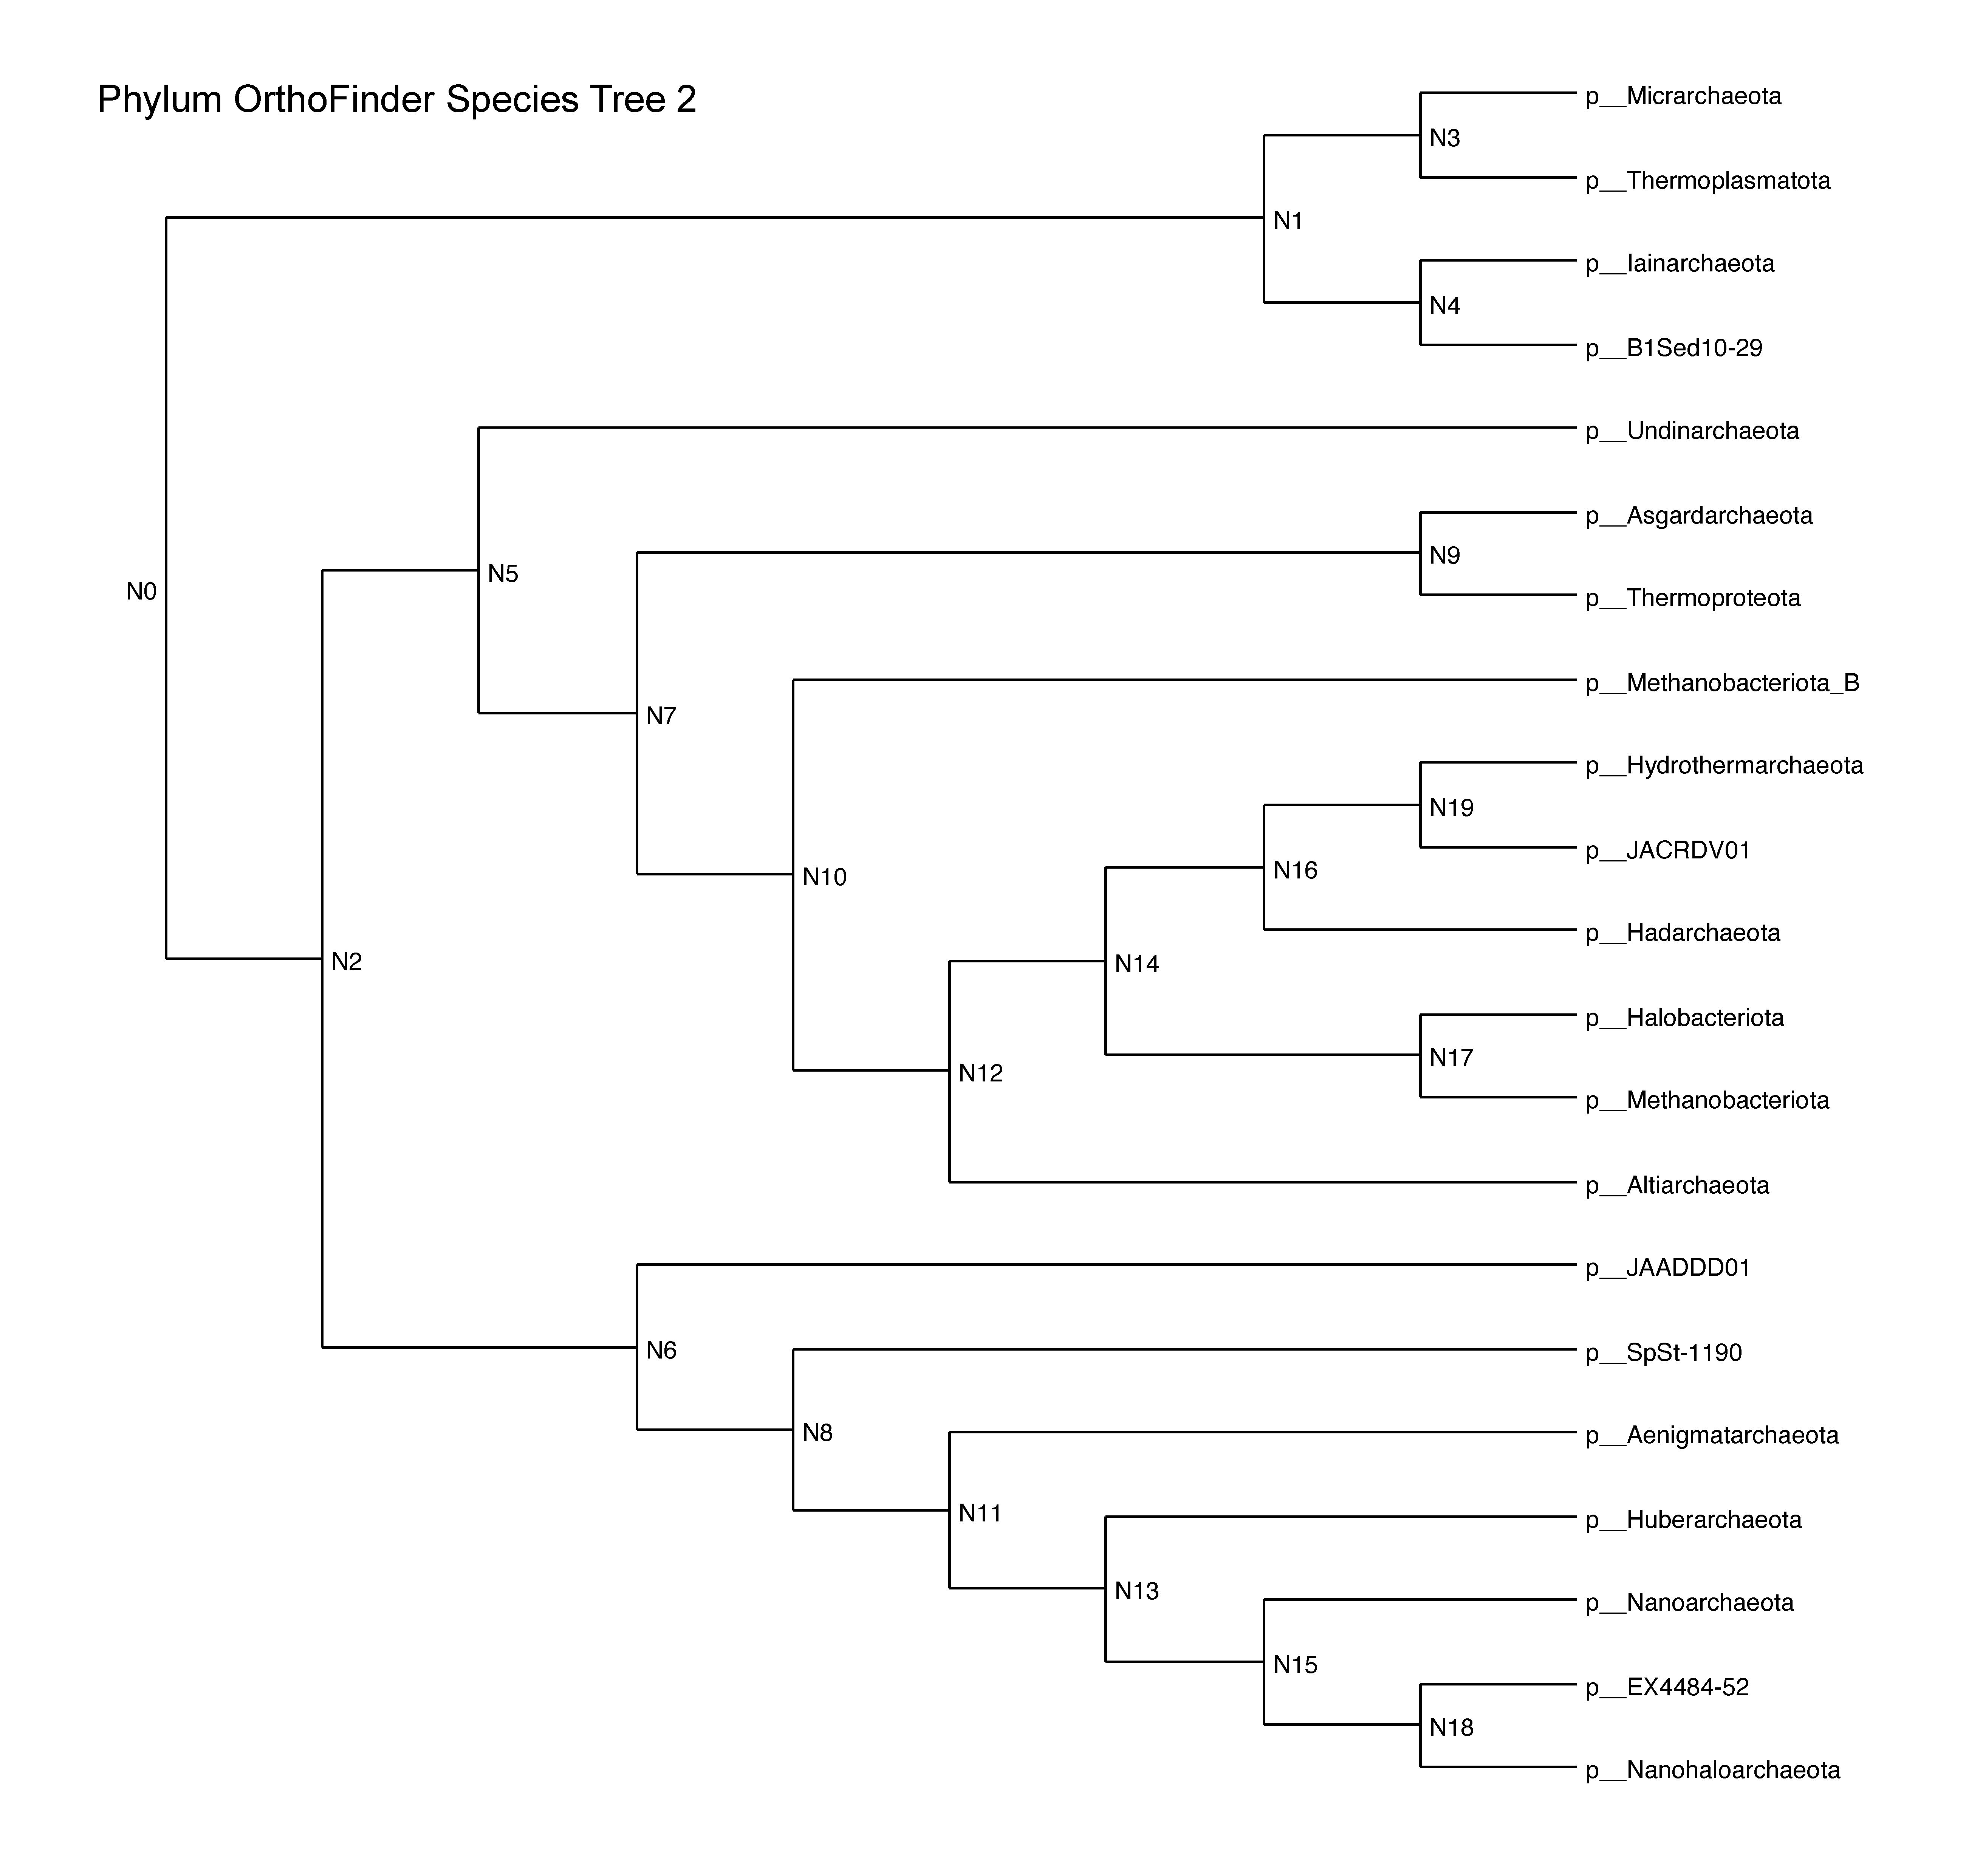
\includegraphics[width=0.5\textwidth]{trees/phy2arc}
    \caption{OrthoFinder-inferred species tree; second analysis.}
    \label{phylum_trees2}
\end{figure}

\begin{figure}[h!tbp]
    \centering
    \renewcommand{\thefigure}{A\arabic{figure}}
    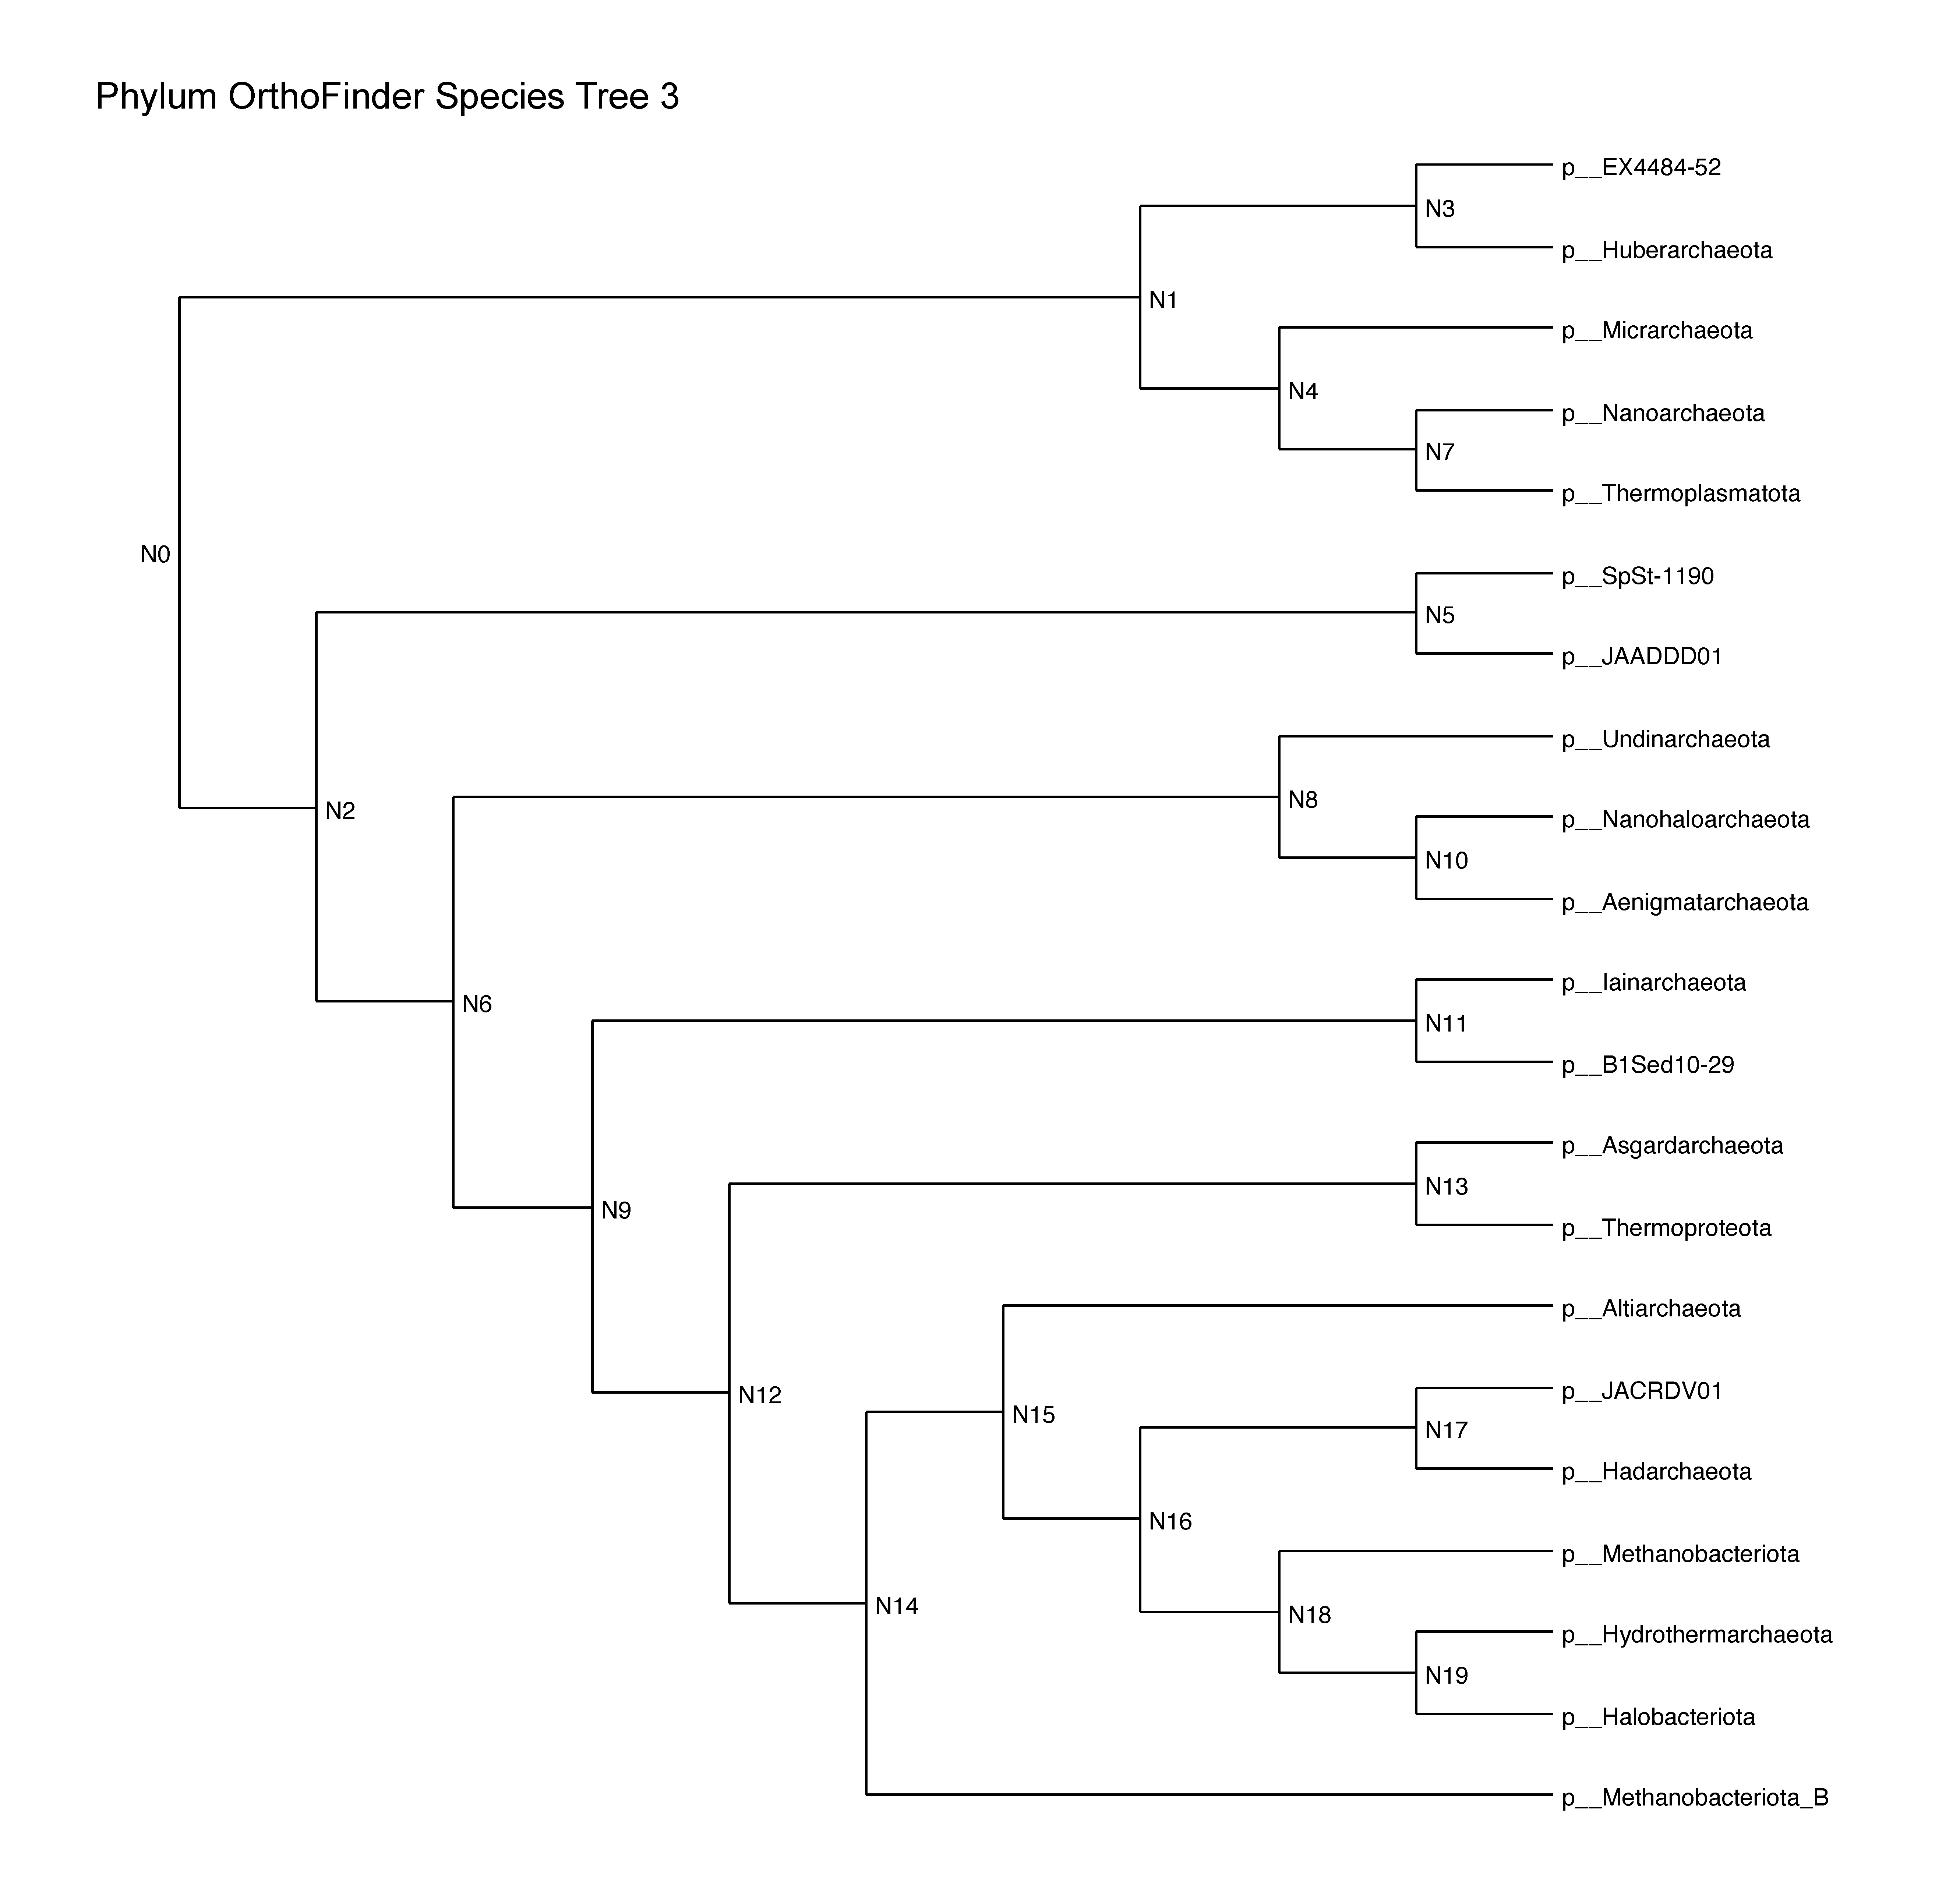
\includegraphics[width=0.6\textwidth]{trees/phy3arc}
    \caption{OrthoFinder-inferred species tree; third analysis.}
    \label{phylum_trees3}
\end{figure}

\begin{figure}[h!tbp]
    \centering
    \renewcommand{\thefigure}{A\arabic{figure}}
    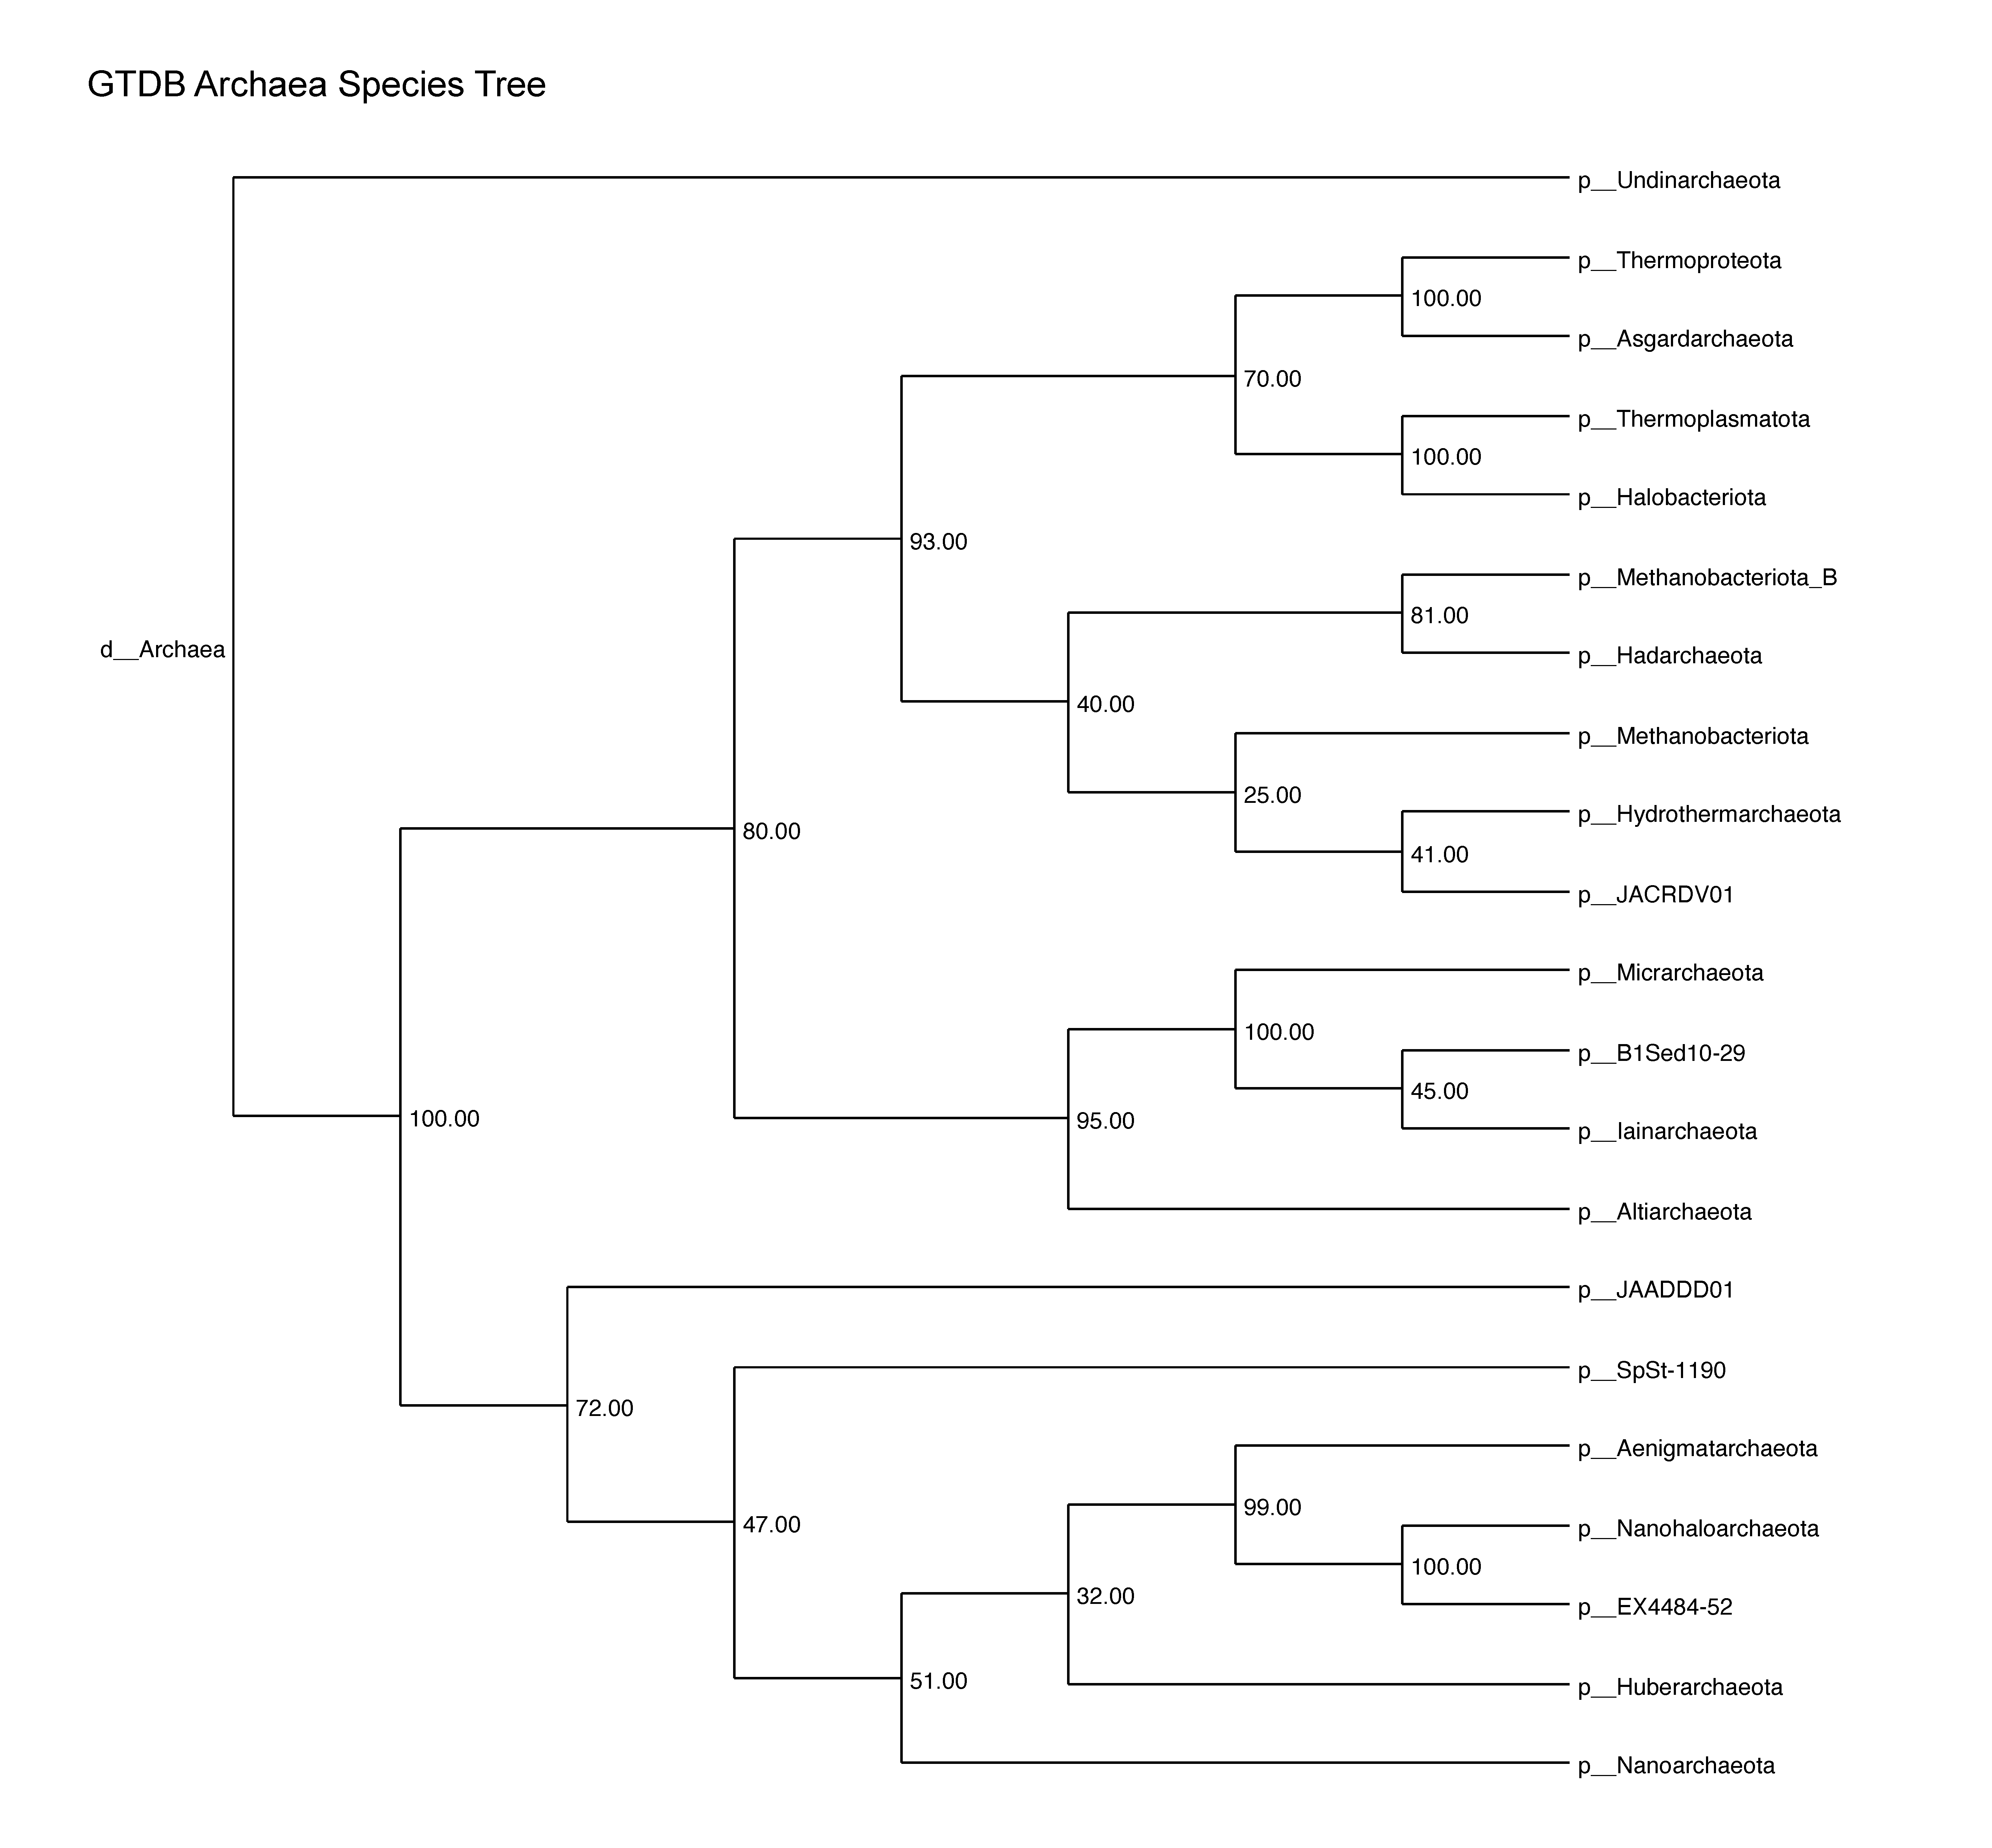
\includegraphics[width=0.6\textwidth]{trees/gtdb_tree}
    \caption{GTDB archaea species tree.}
    \label{gtdb_tree}
\end{figure}

\newpage
\subsection*{A2. Metabolic Network Reconstruction of LACA for all Archaea Datasets}
\textbf{Metabolic Potential of LACA.}

\begin{figure}[H]
    \centering
    \includegraphics[width=0.95\textwidth]{metabolism/phy_arc_n0.pdf}
    \caption{Reconstruction of LACA's metabolic network from extant life, for the phylum-level archaea dataset. In black: enzymes and metabolic pathways that were inferred to be present in LACA.}
    \label{phy4arc_metnet}
\end{figure}   

\begin{figure}[H]
    \centering
    \includegraphics[width=0.95\textwidth]{metabolism/cla_arc_n0.pdf}
    \caption{Reconstruction of LACA's metabolic network from extant life, for the class-level archaea dataset. In black: enzymes and metabolic pathways that were inferred to be present in LACA.}
    \label{cla4arc_metnet}
\end{figure}   

\begin{figure}[H]
    \centering
    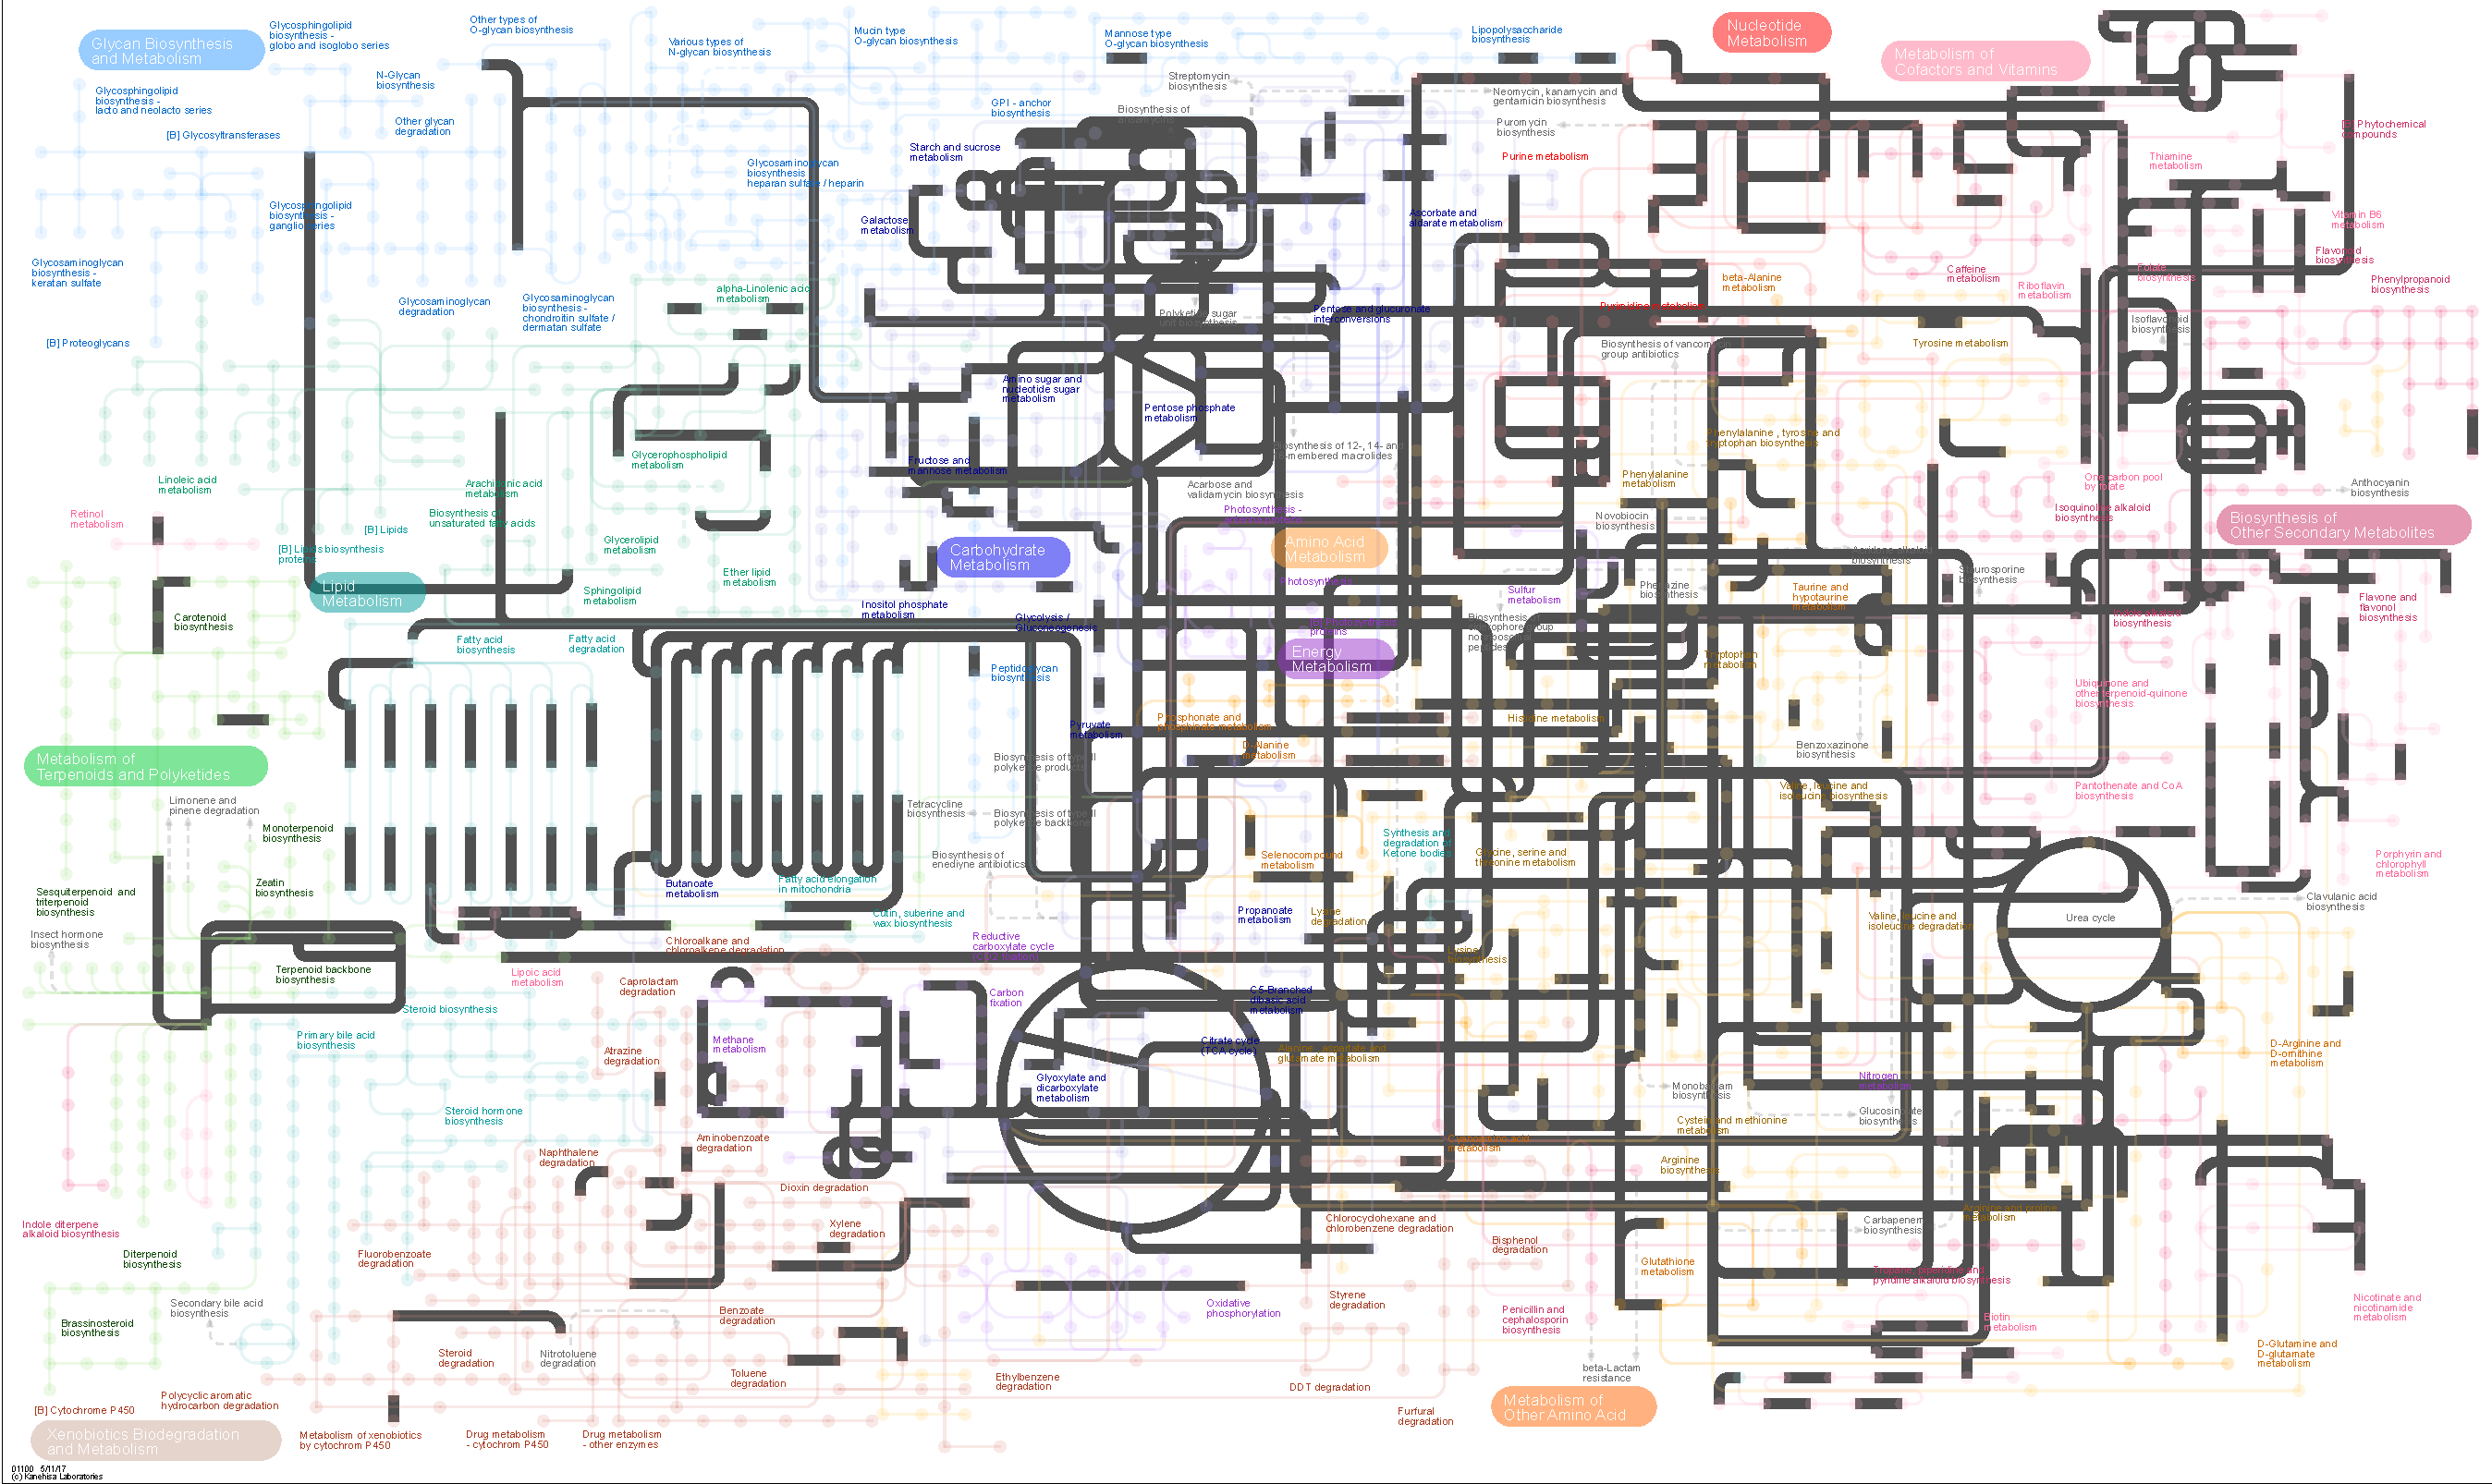
\includegraphics[width=0.95\textwidth]{metabolism/ord_arc_n0.pdf}
    \caption{Reconstruction of LACA's metabolic network from extant life, for the order-level archaea dataset. In black: enzymes and metabolic pathways that were inferred to be present in LACA.}
    \label{ord4arc_metnet}
\end{figure}   

\begin{figure}[H]
    \centering
    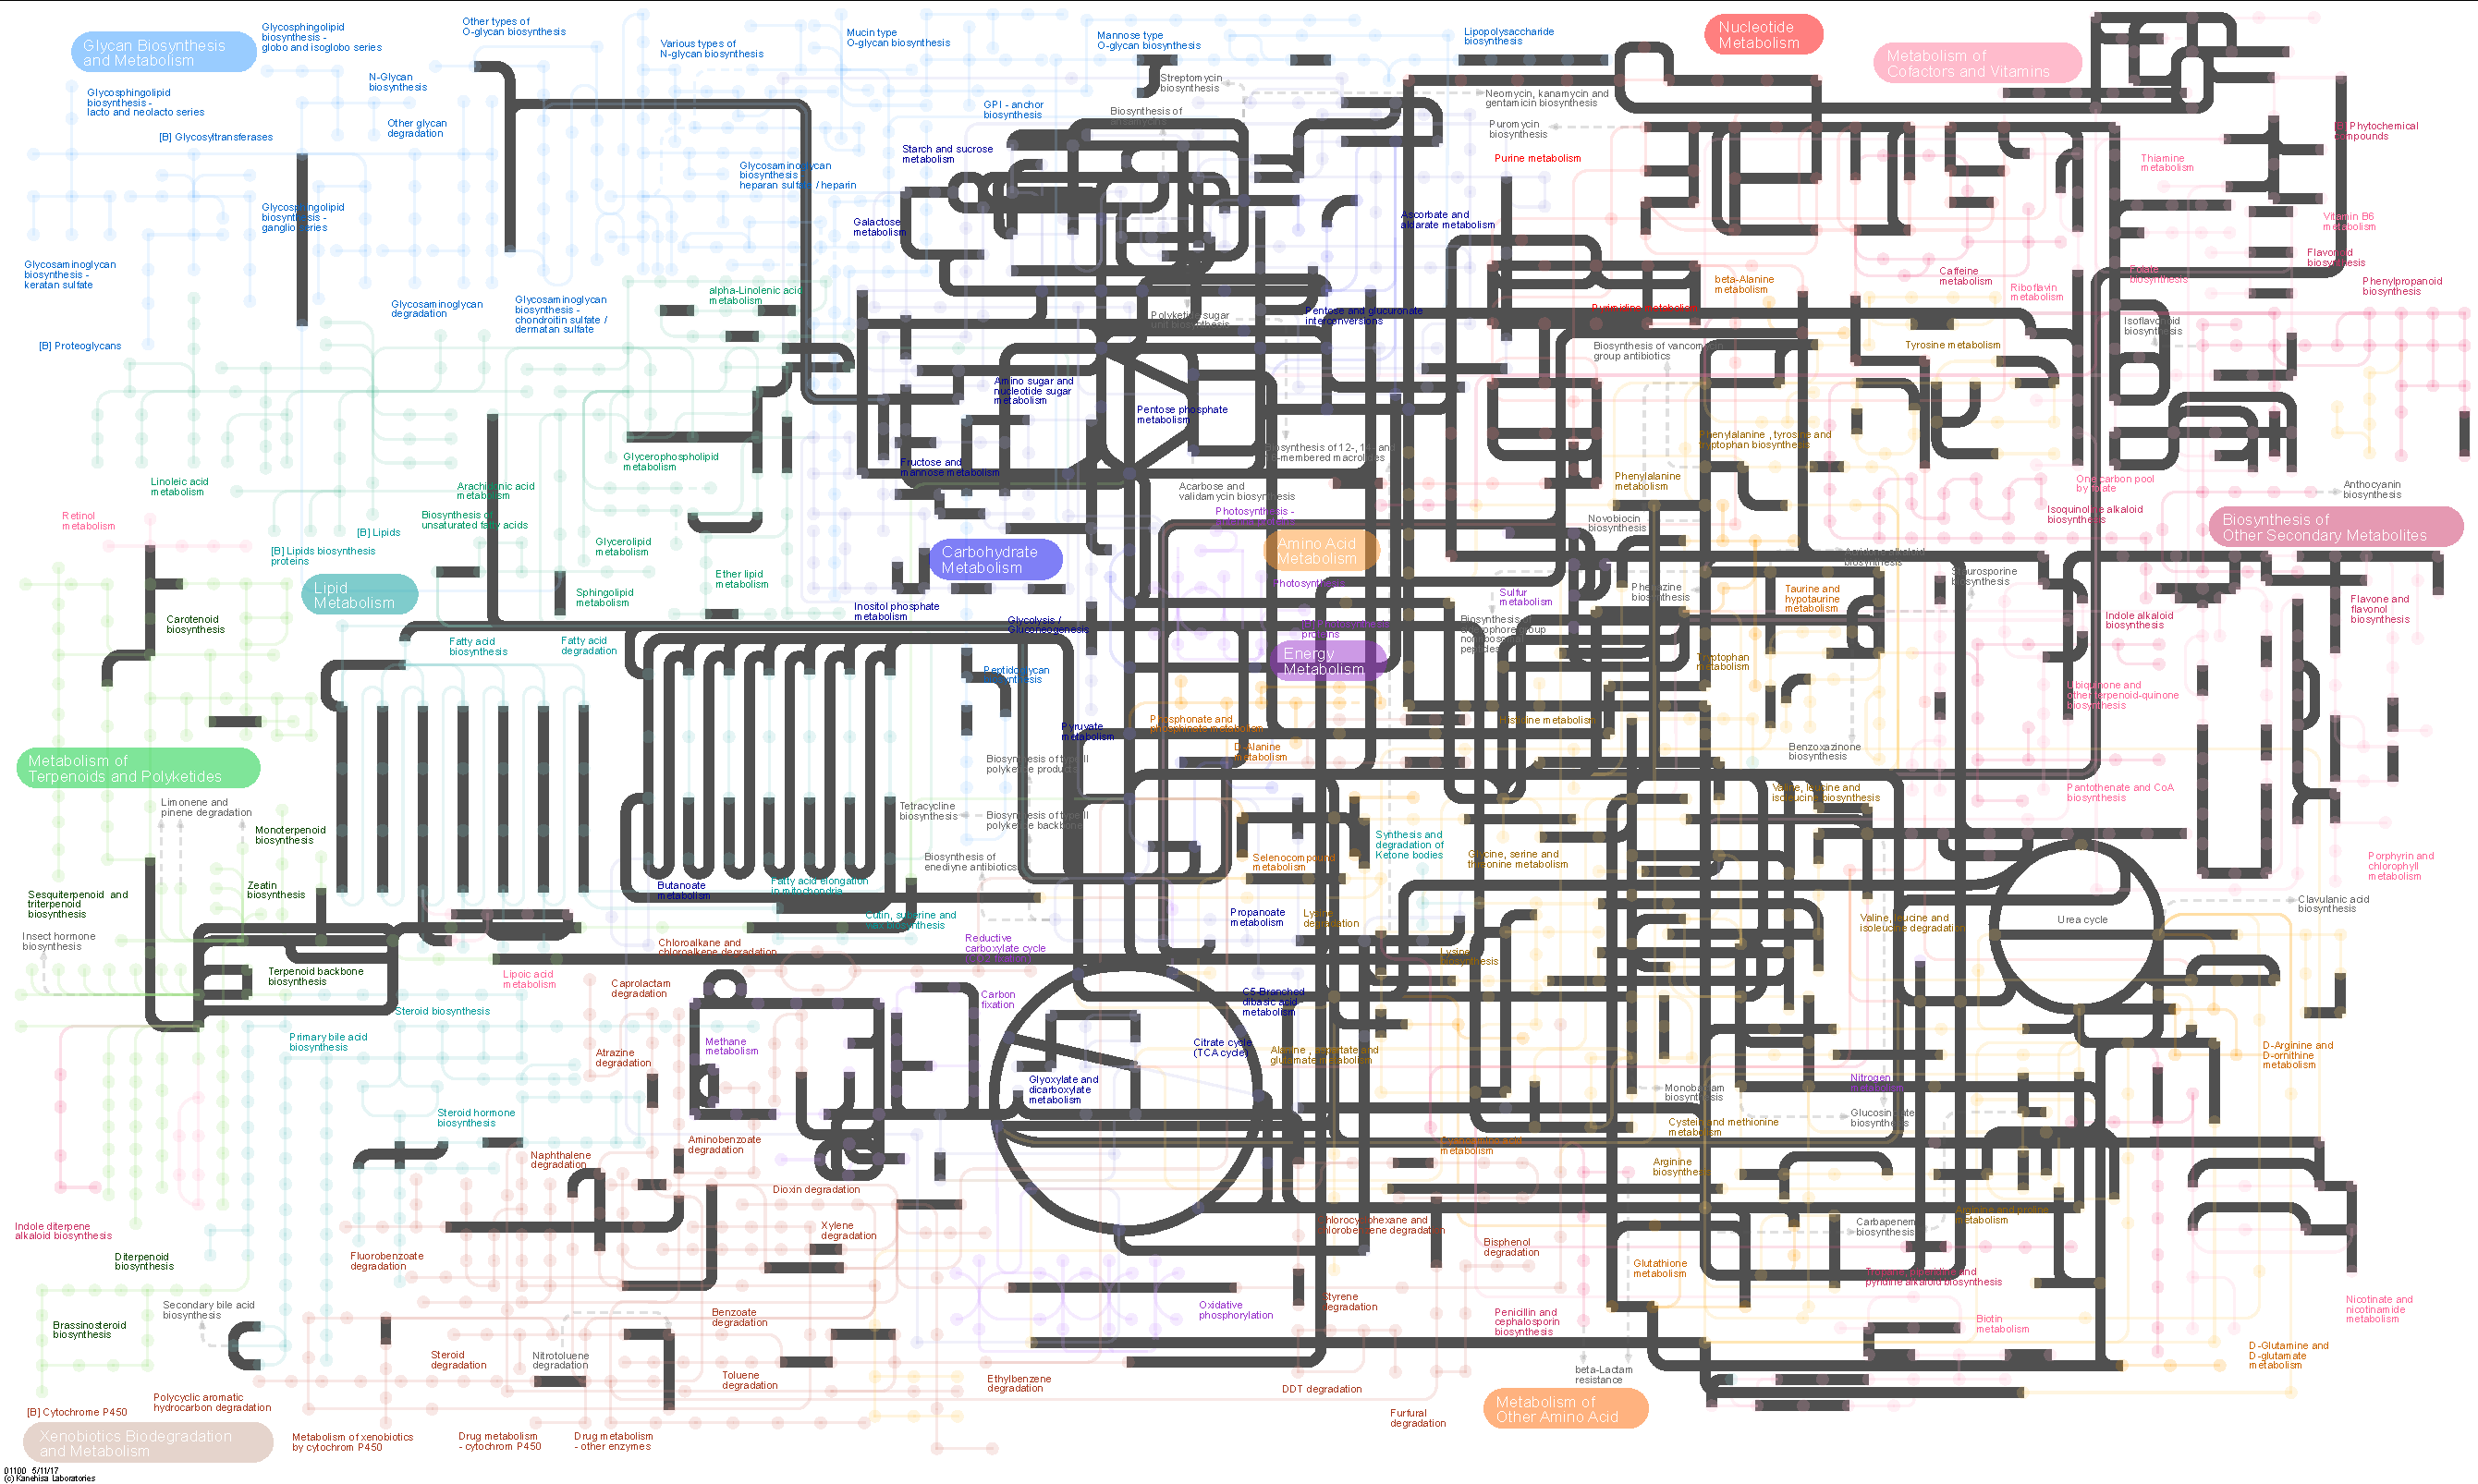
\includegraphics[width=0.95\textwidth]{metabolism/gen_arc_n0.pdf}
    \caption{Reconstruction of LACA's metabolic network from extant life, for the genus-level archaea dataset. In black: enzymes and metabolic pathways that were inferred to be present in LACA.}
    \label{gen4arc_metnet}
\end{figure}   


\begin{figure}[H]
    \centering
    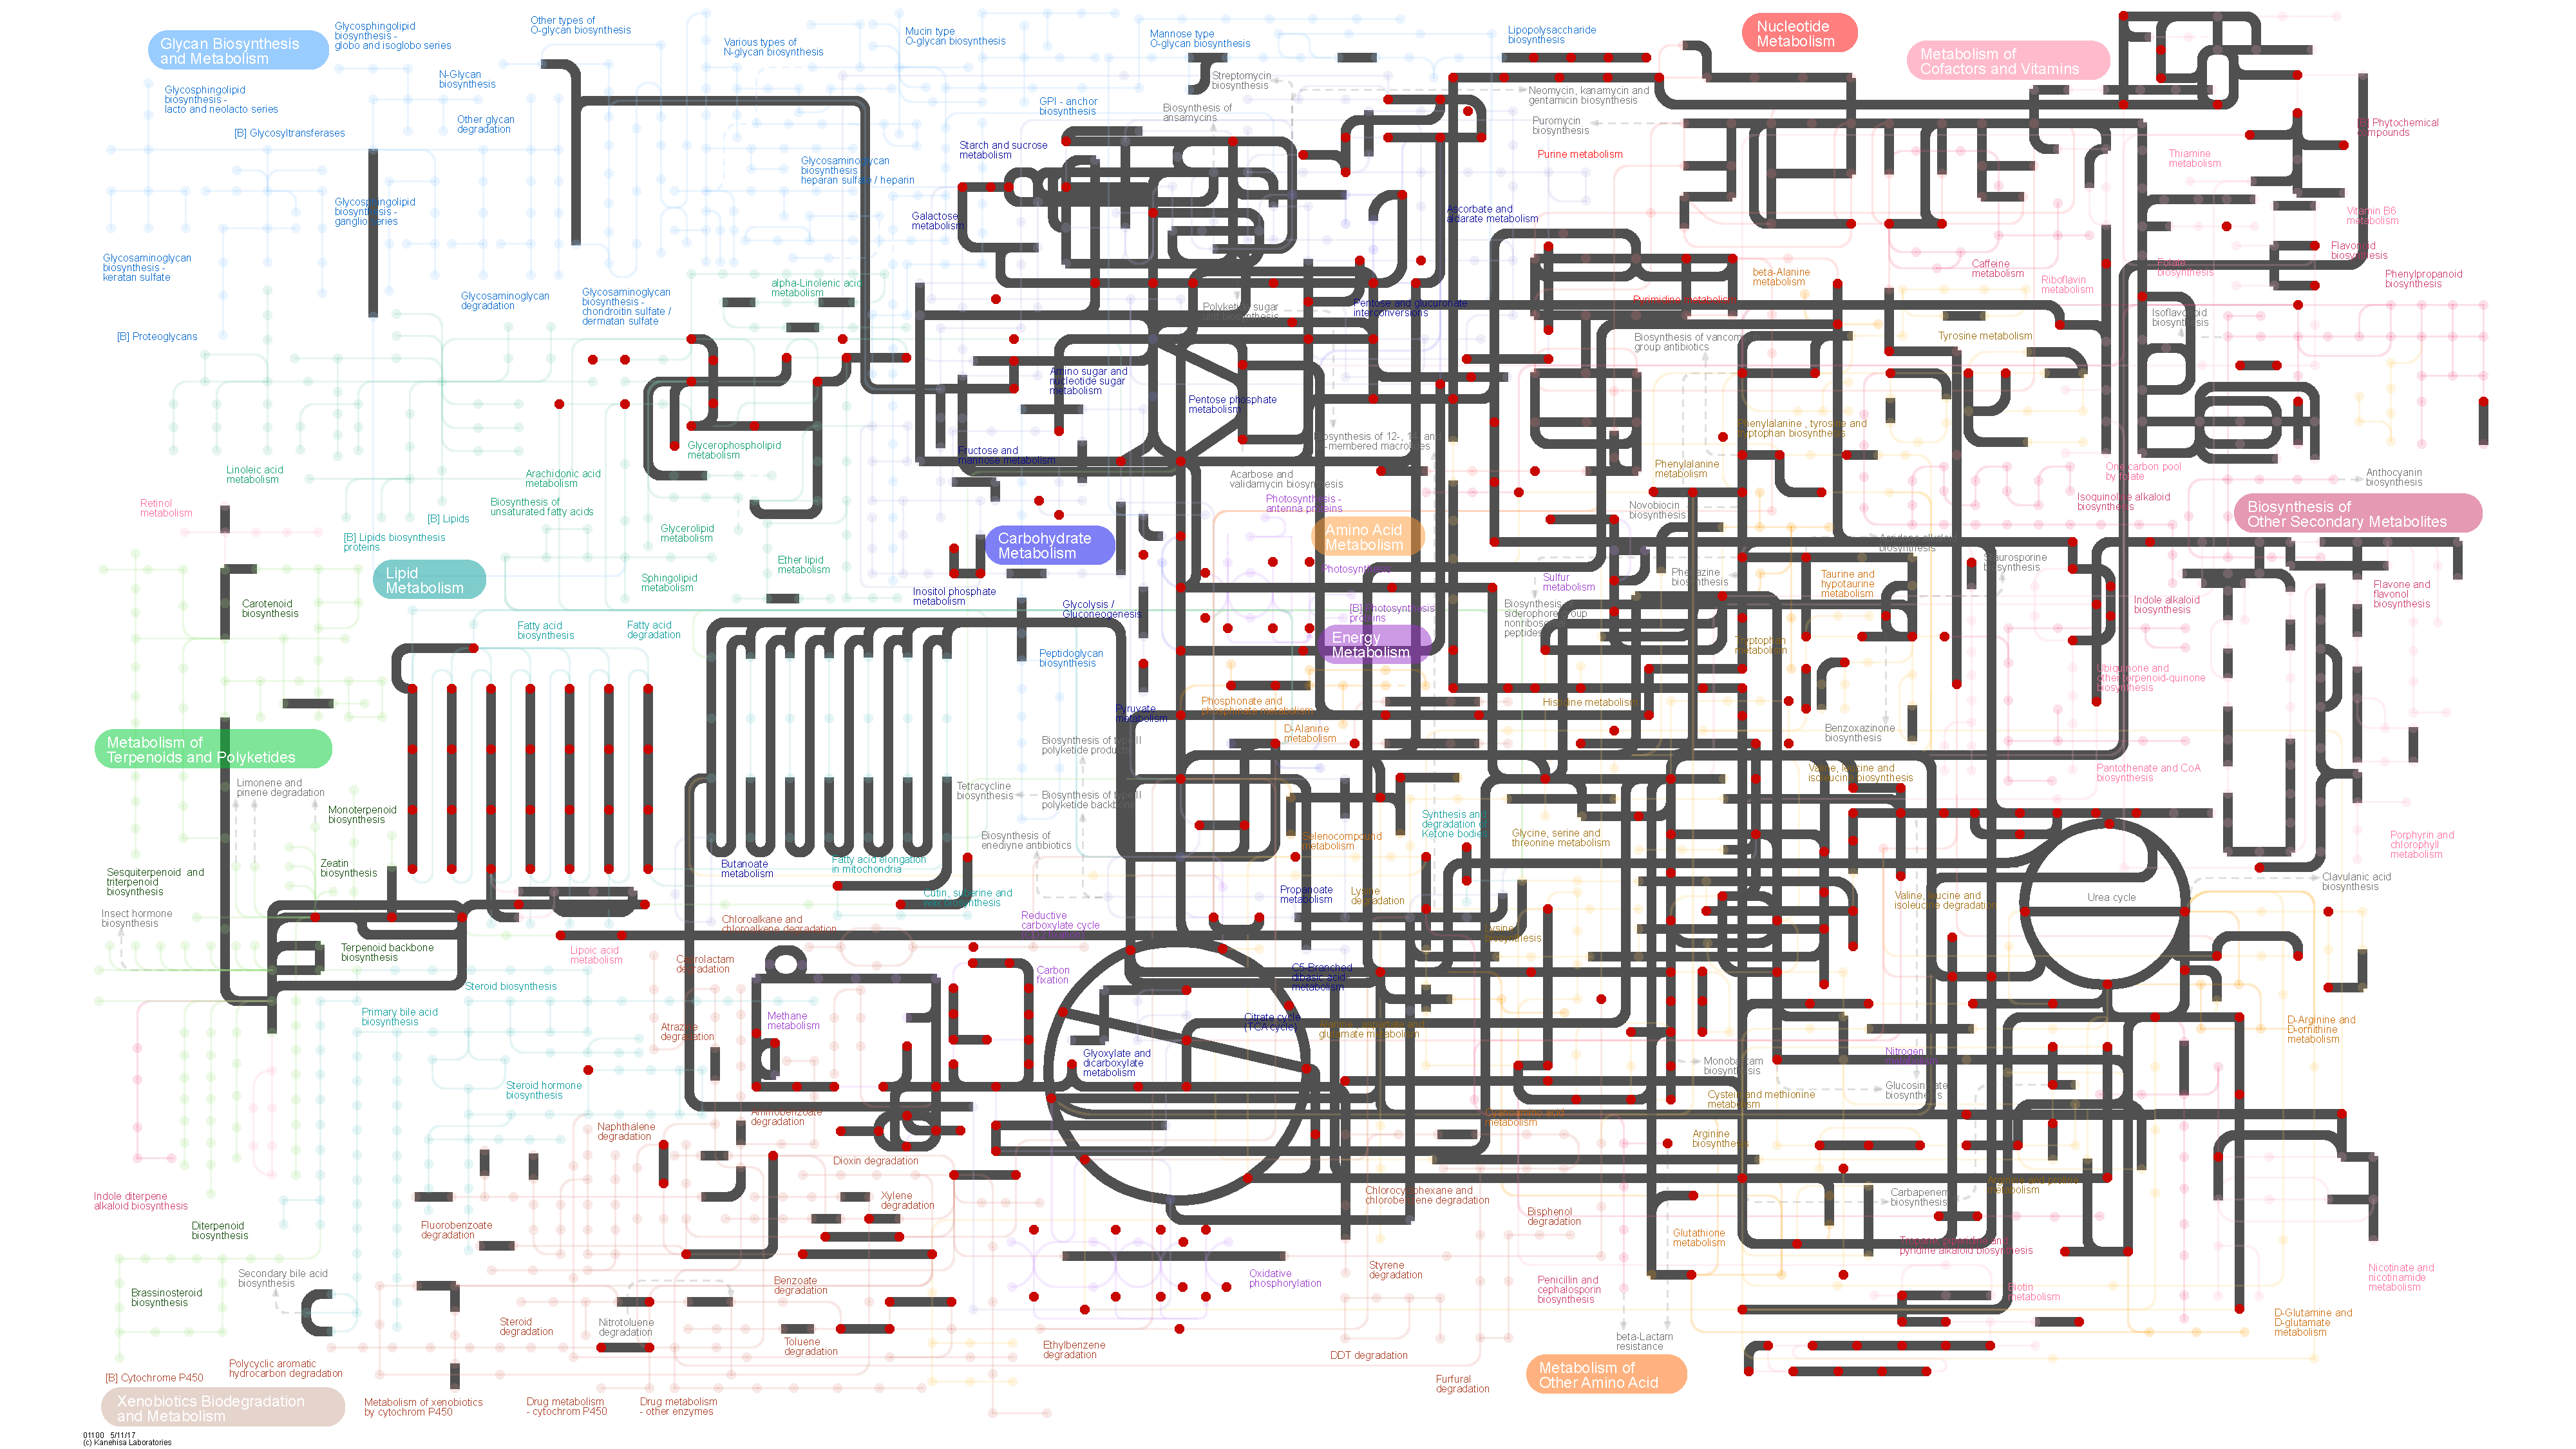
\includegraphics[width=0.95\textwidth]{metabolism/fam_N0_plus_06seedset.pdf}
    \caption{Reconstruction of LACA's metabolic network from extant life, for the family-level archaea dataset. In black: enzymes and metabolic pathways that were inferred to be present in LACA. Red dots: seed compounds of 60\% completeness seed set.}
    \label{fam4arc_metnet_plus_seedset}
\end{figure}   

\newpage
\textbf{EC number evolution in LACA.}
\begin{figure}[H]
    \centering
    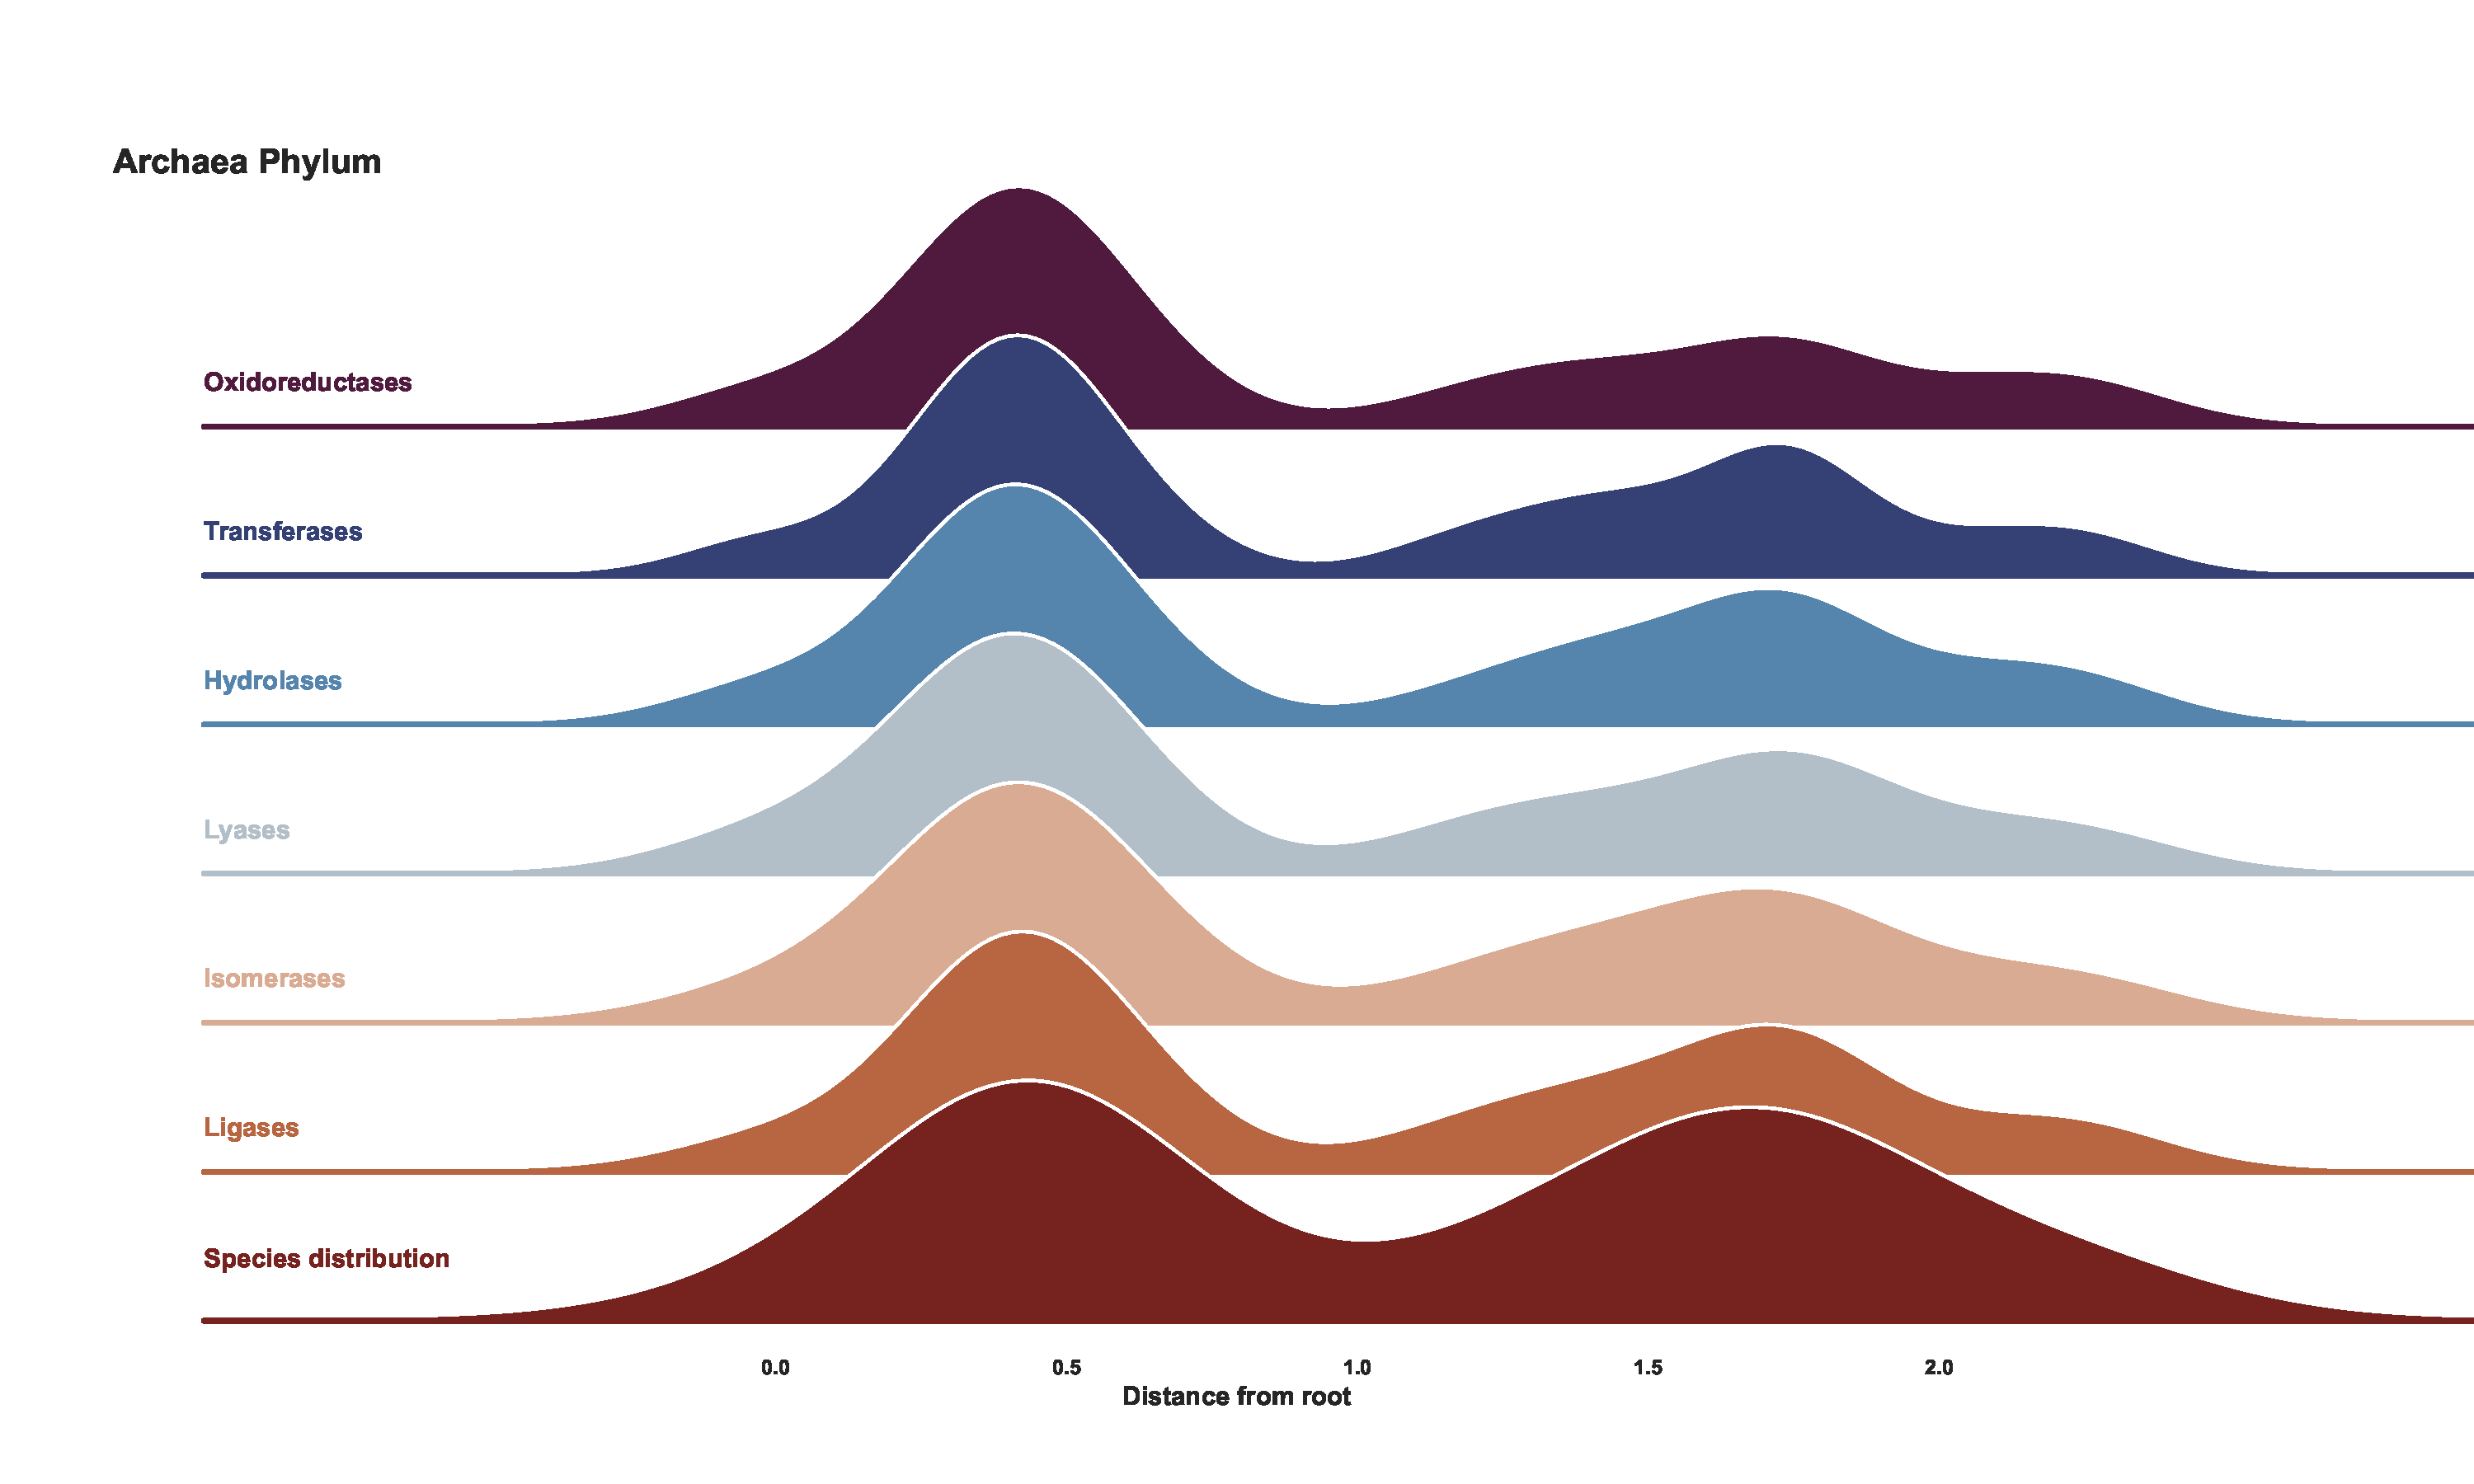
\includegraphics[width=0.95\textwidth]{ridgeplots/phy4arc_ridgeplot.pdf}
    \label{ridgeplot_phy4arc}
\end{figure}

\begin{figure}[H]
    \centering
    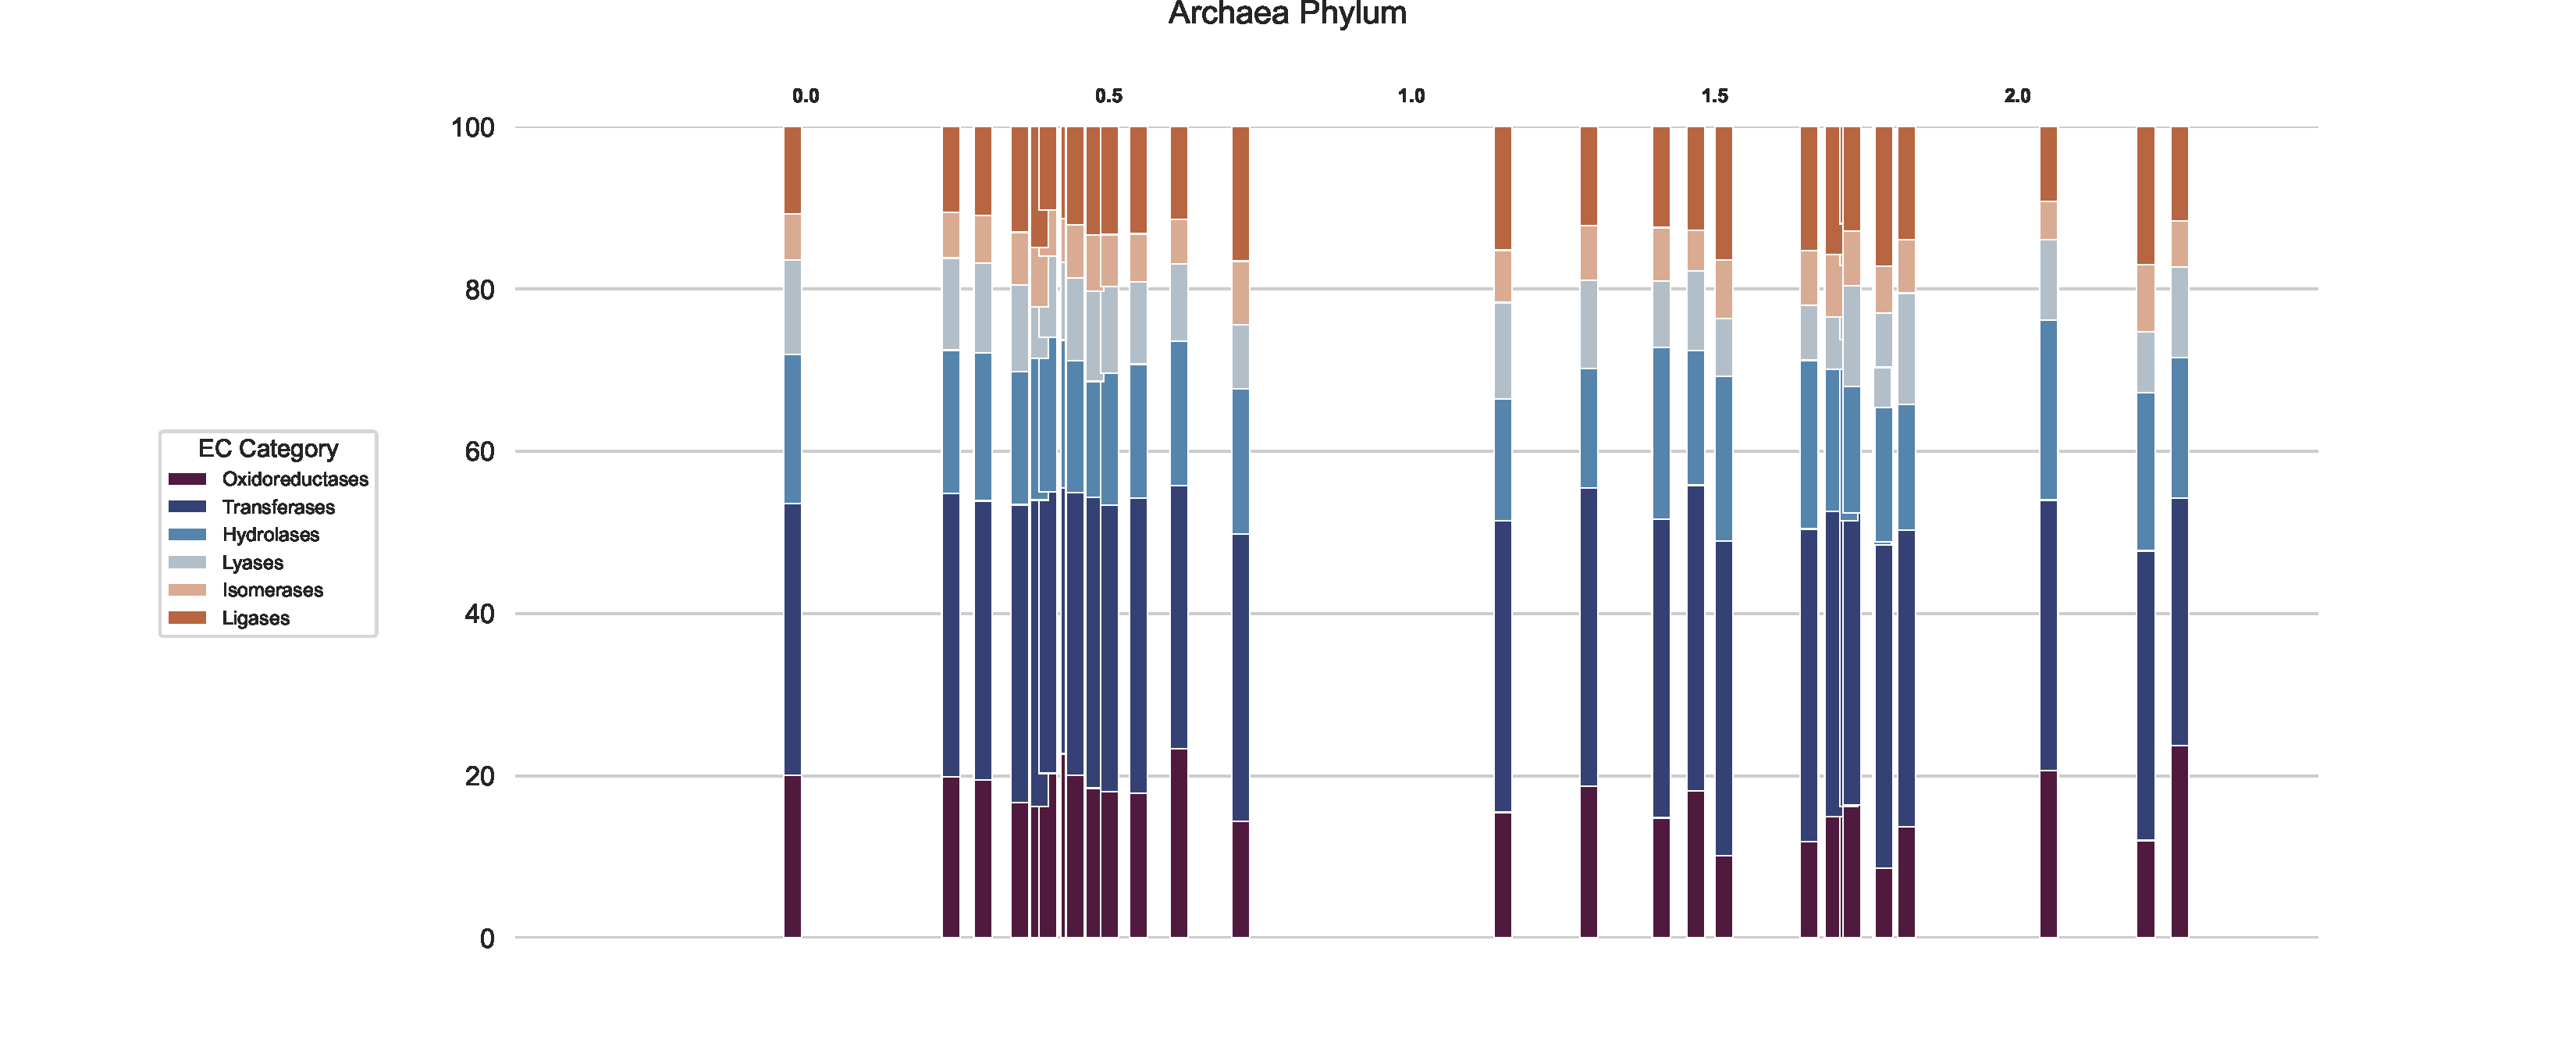
\includegraphics[width=0.95\textwidth]{ridgeplots/phy4arc_barplot.pdf}
    \caption[]{Evolution of individual enzyme categories for the phylum-level archaea dataset. The ridgeplot displays the distribution of each category as a function of distance from the tree root, with the last axis presenting the species distribution, while the barplot the relative abundance of each category at that particular distance as a stacked barplot.}
    \label{barplot_phy4arc}
\end{figure}

\begin{figure}[H]
    \centering
    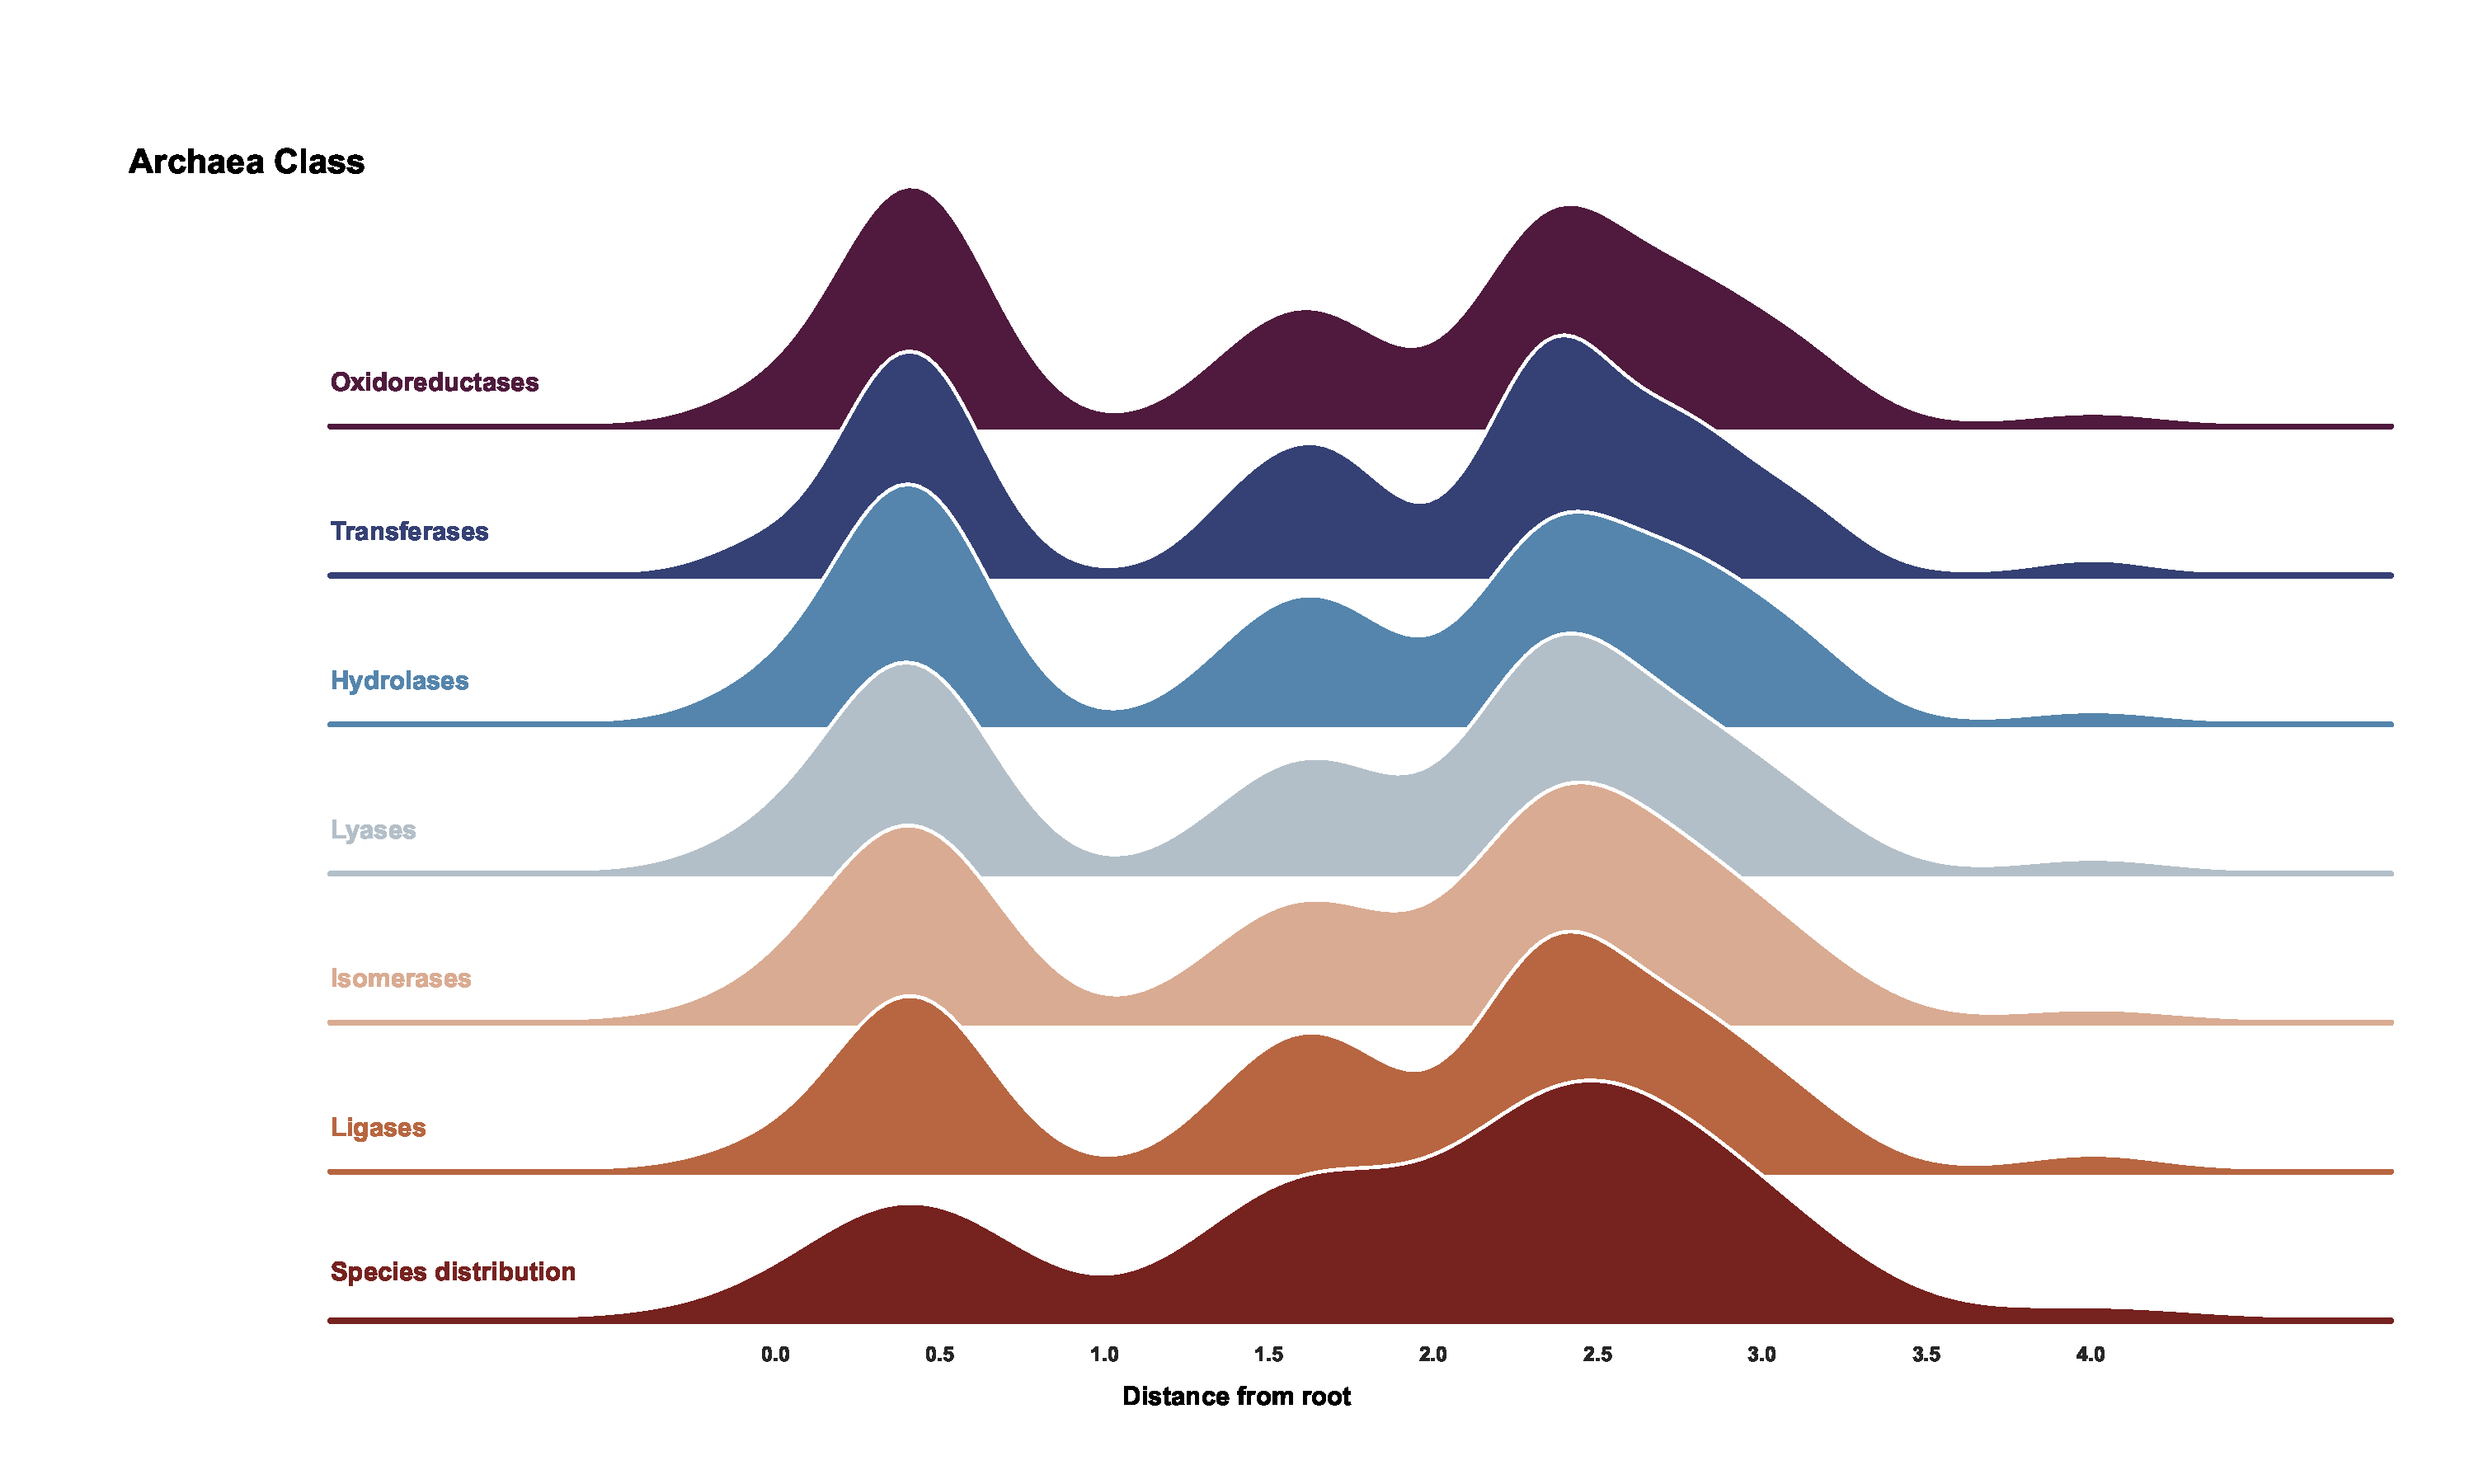
\includegraphics[width=0.95\textwidth]{ridgeplots/cla4arc_ridgeplot.pdf}
    \label{ridgeplot_cla4arc}
\end{figure}

\begin{figure}[H]
    \centering
    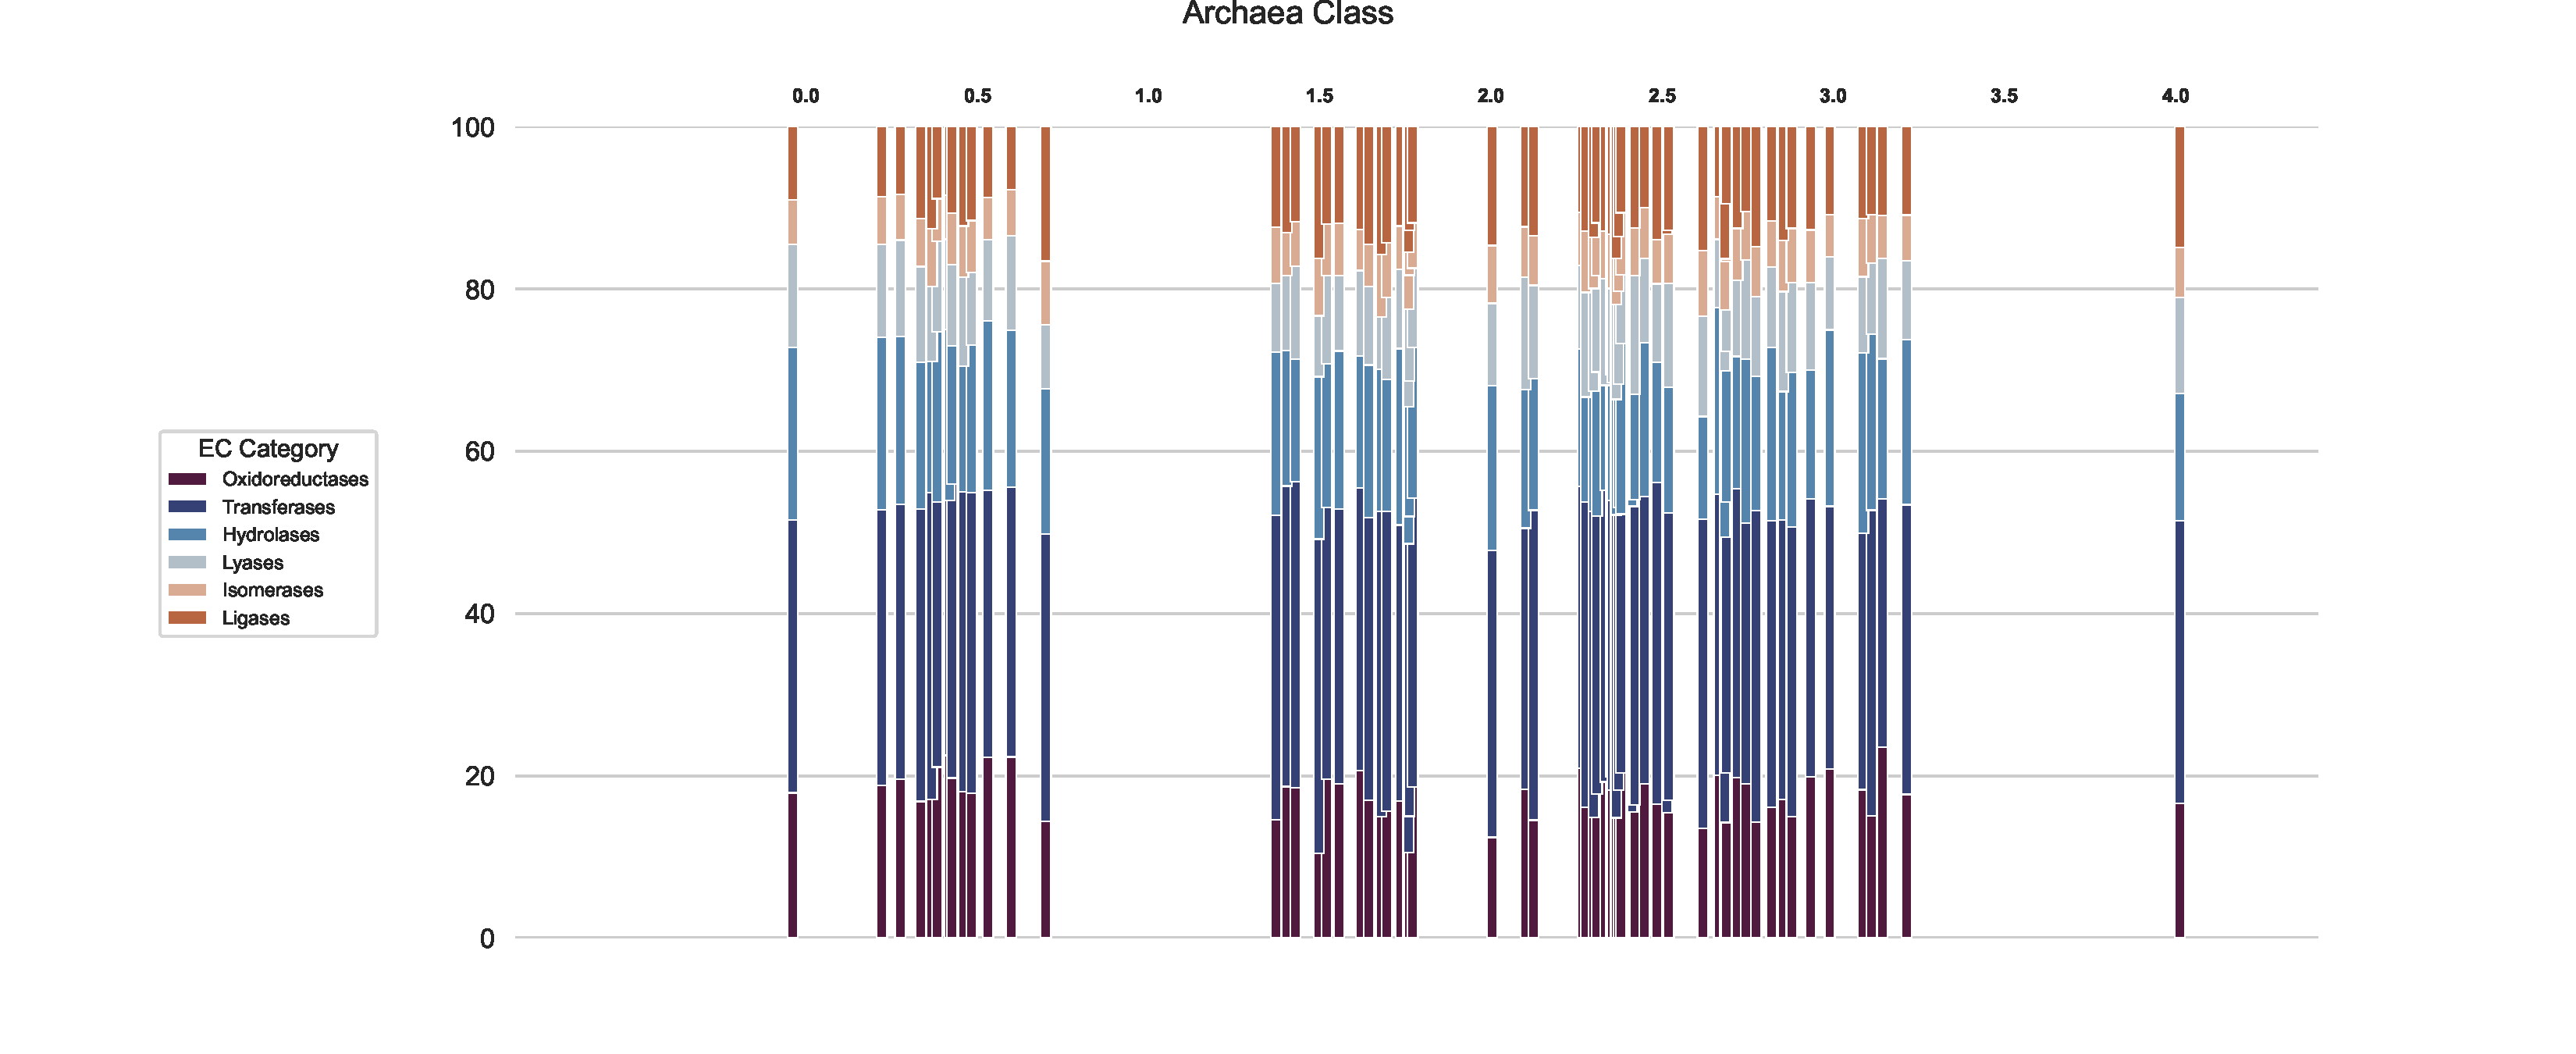
\includegraphics[width=0.95\textwidth]{ridgeplots/cla4arc_barplot.pdf}
    \caption[]{Evolution of individual enzyme categories for the class-level archaea dataset. The ridgeplot displays the distribution of each category as a function of distance from the tree root, with the last axis presenting the species distribution, while the barplot the relative abundance of each category at that particular distance as a stacked barplot.}
    \label{barplot_cla4arc}
\end{figure}

\begin{figure}[H]
    \centering
    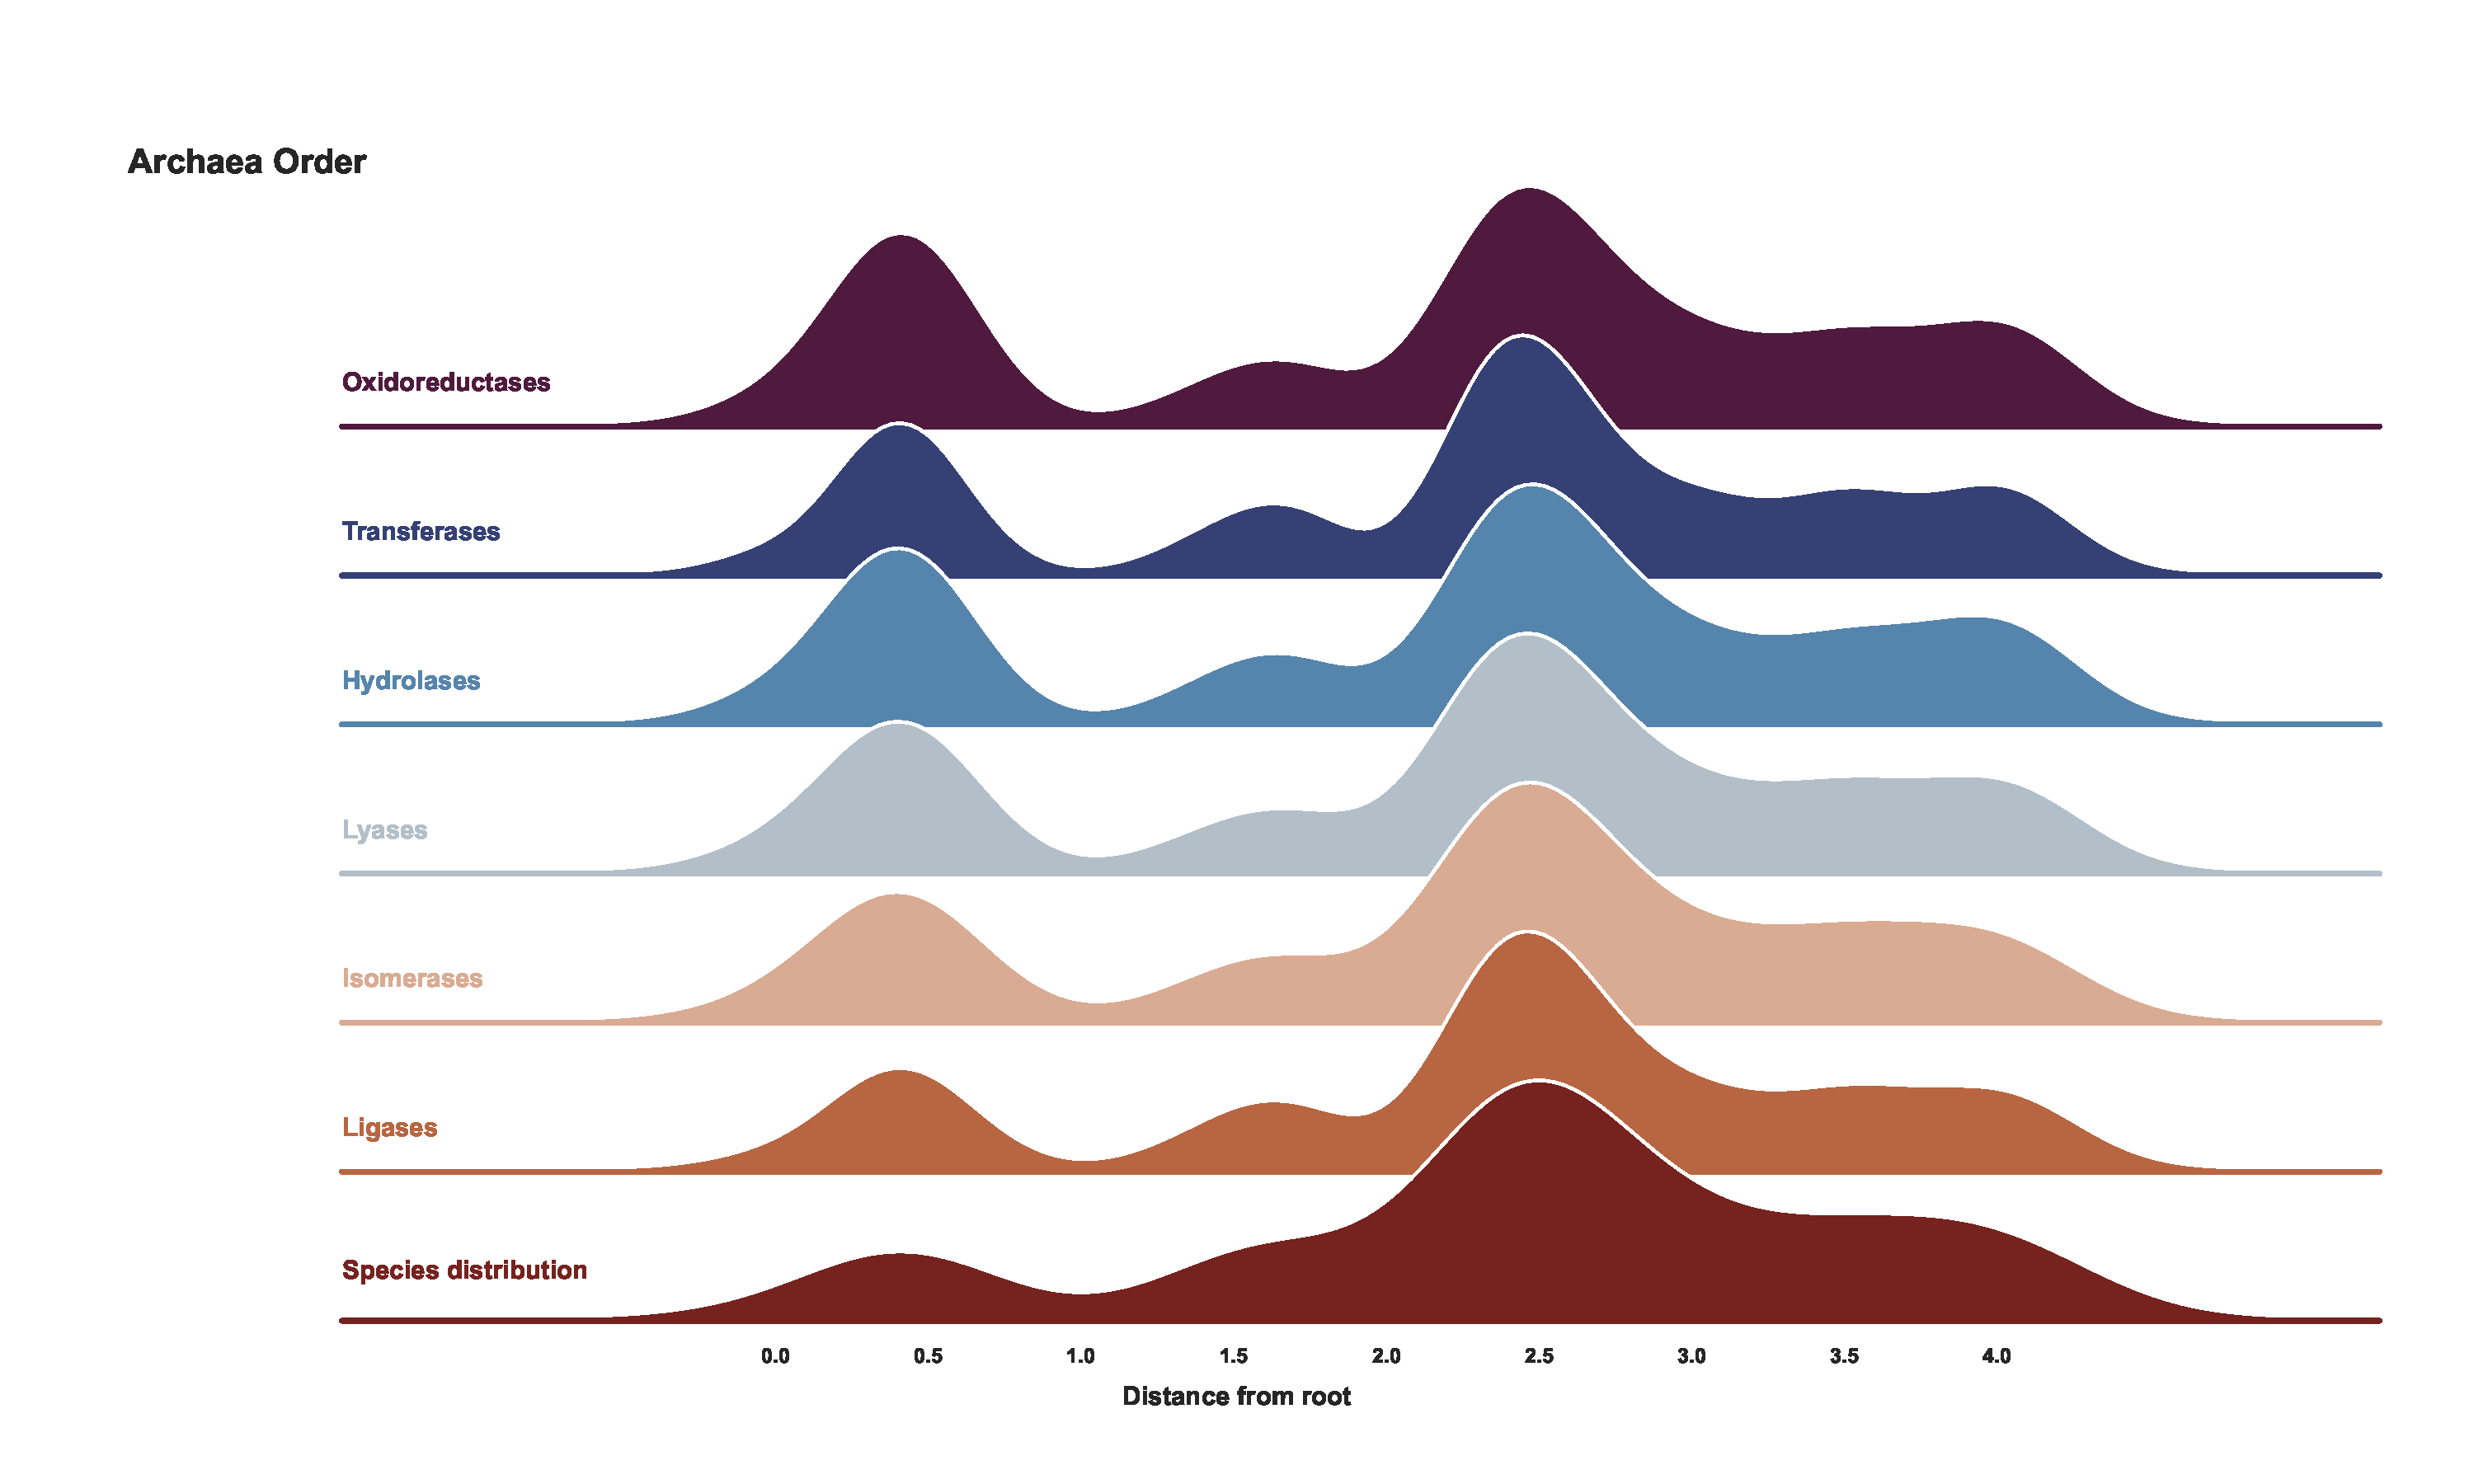
\includegraphics[width=0.95\textwidth]{ridgeplots/ord4arc_ridgeplot.pdf}
    \label{ridgeplot_ord4arc}
\end{figure}

\begin{figure}[H]
    \centering
    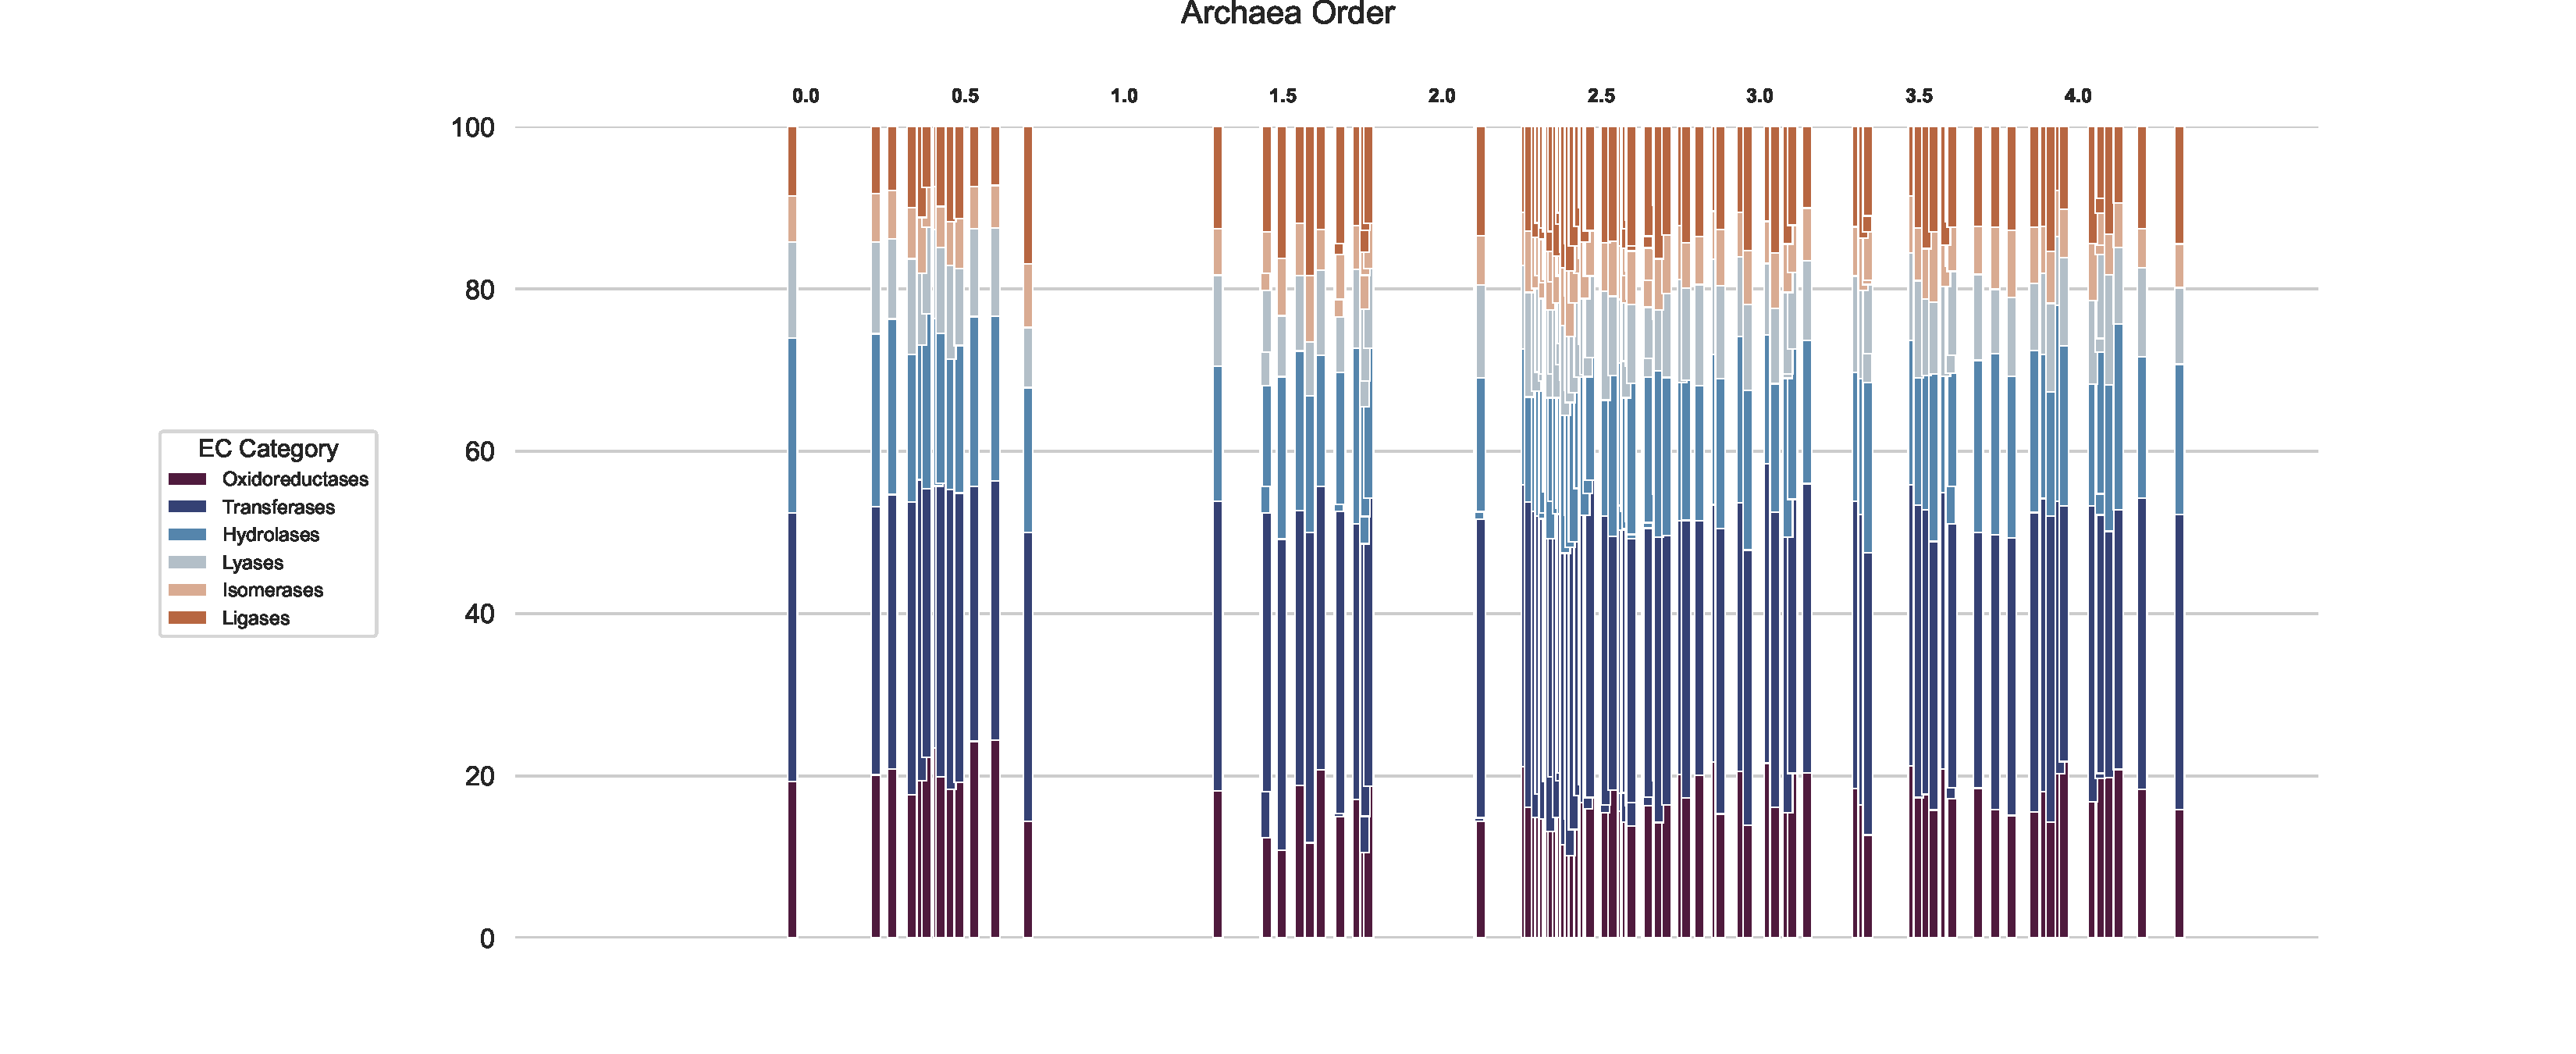
\includegraphics[width=0.95\textwidth]{ridgeplots/ord4arc_barplot.pdf}
    \caption[]{Evolution of individual enzyme categories for the order-level archaea dataset. The ridgeplot displays the distribution of each category as a function of distance from the tree root, with the last axis presenting the species distribution, while the barplot the relative abundance of each category at that particular distance as a stacked barplot.}
    \label{barplot_ord4arc}
\end{figure}

\begin{figure}[H]
    \centering
    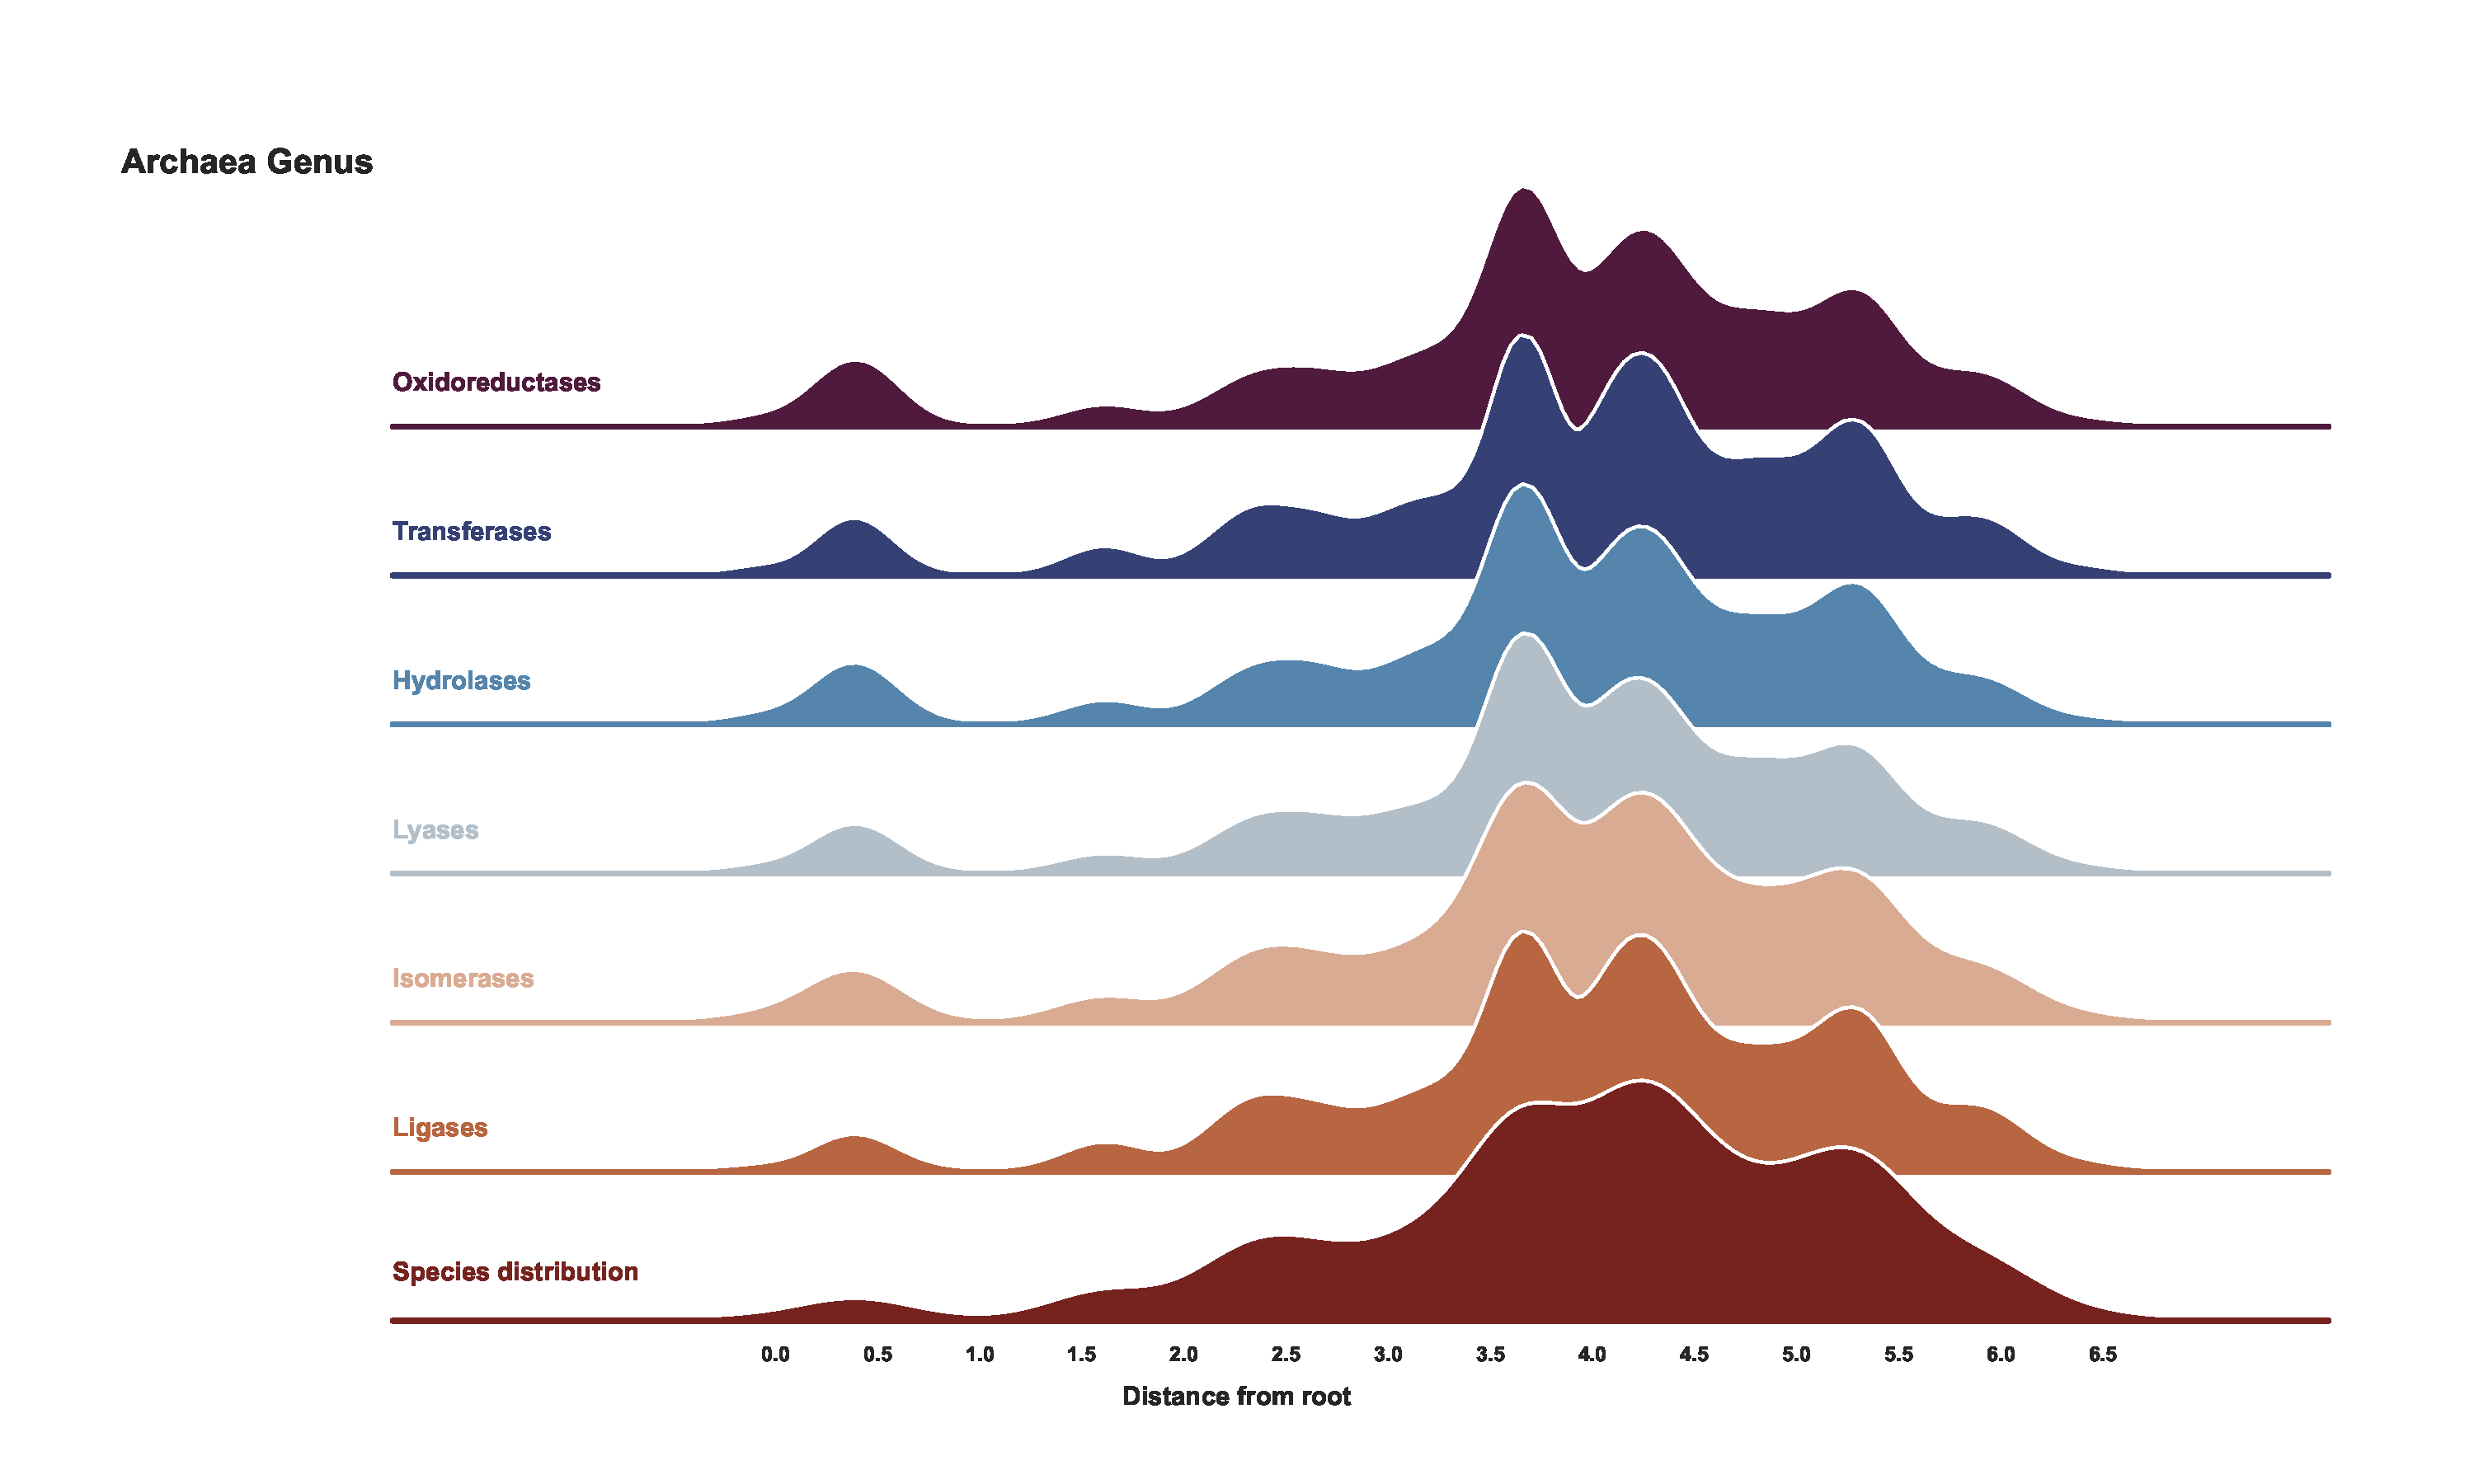
\includegraphics[width=0.95\textwidth]{ridgeplots/gen4arc_ridgeplot.pdf}
    \label{ridgeplot_gen4arc}
\end{figure}

\begin{figure}[H]
    \centering
    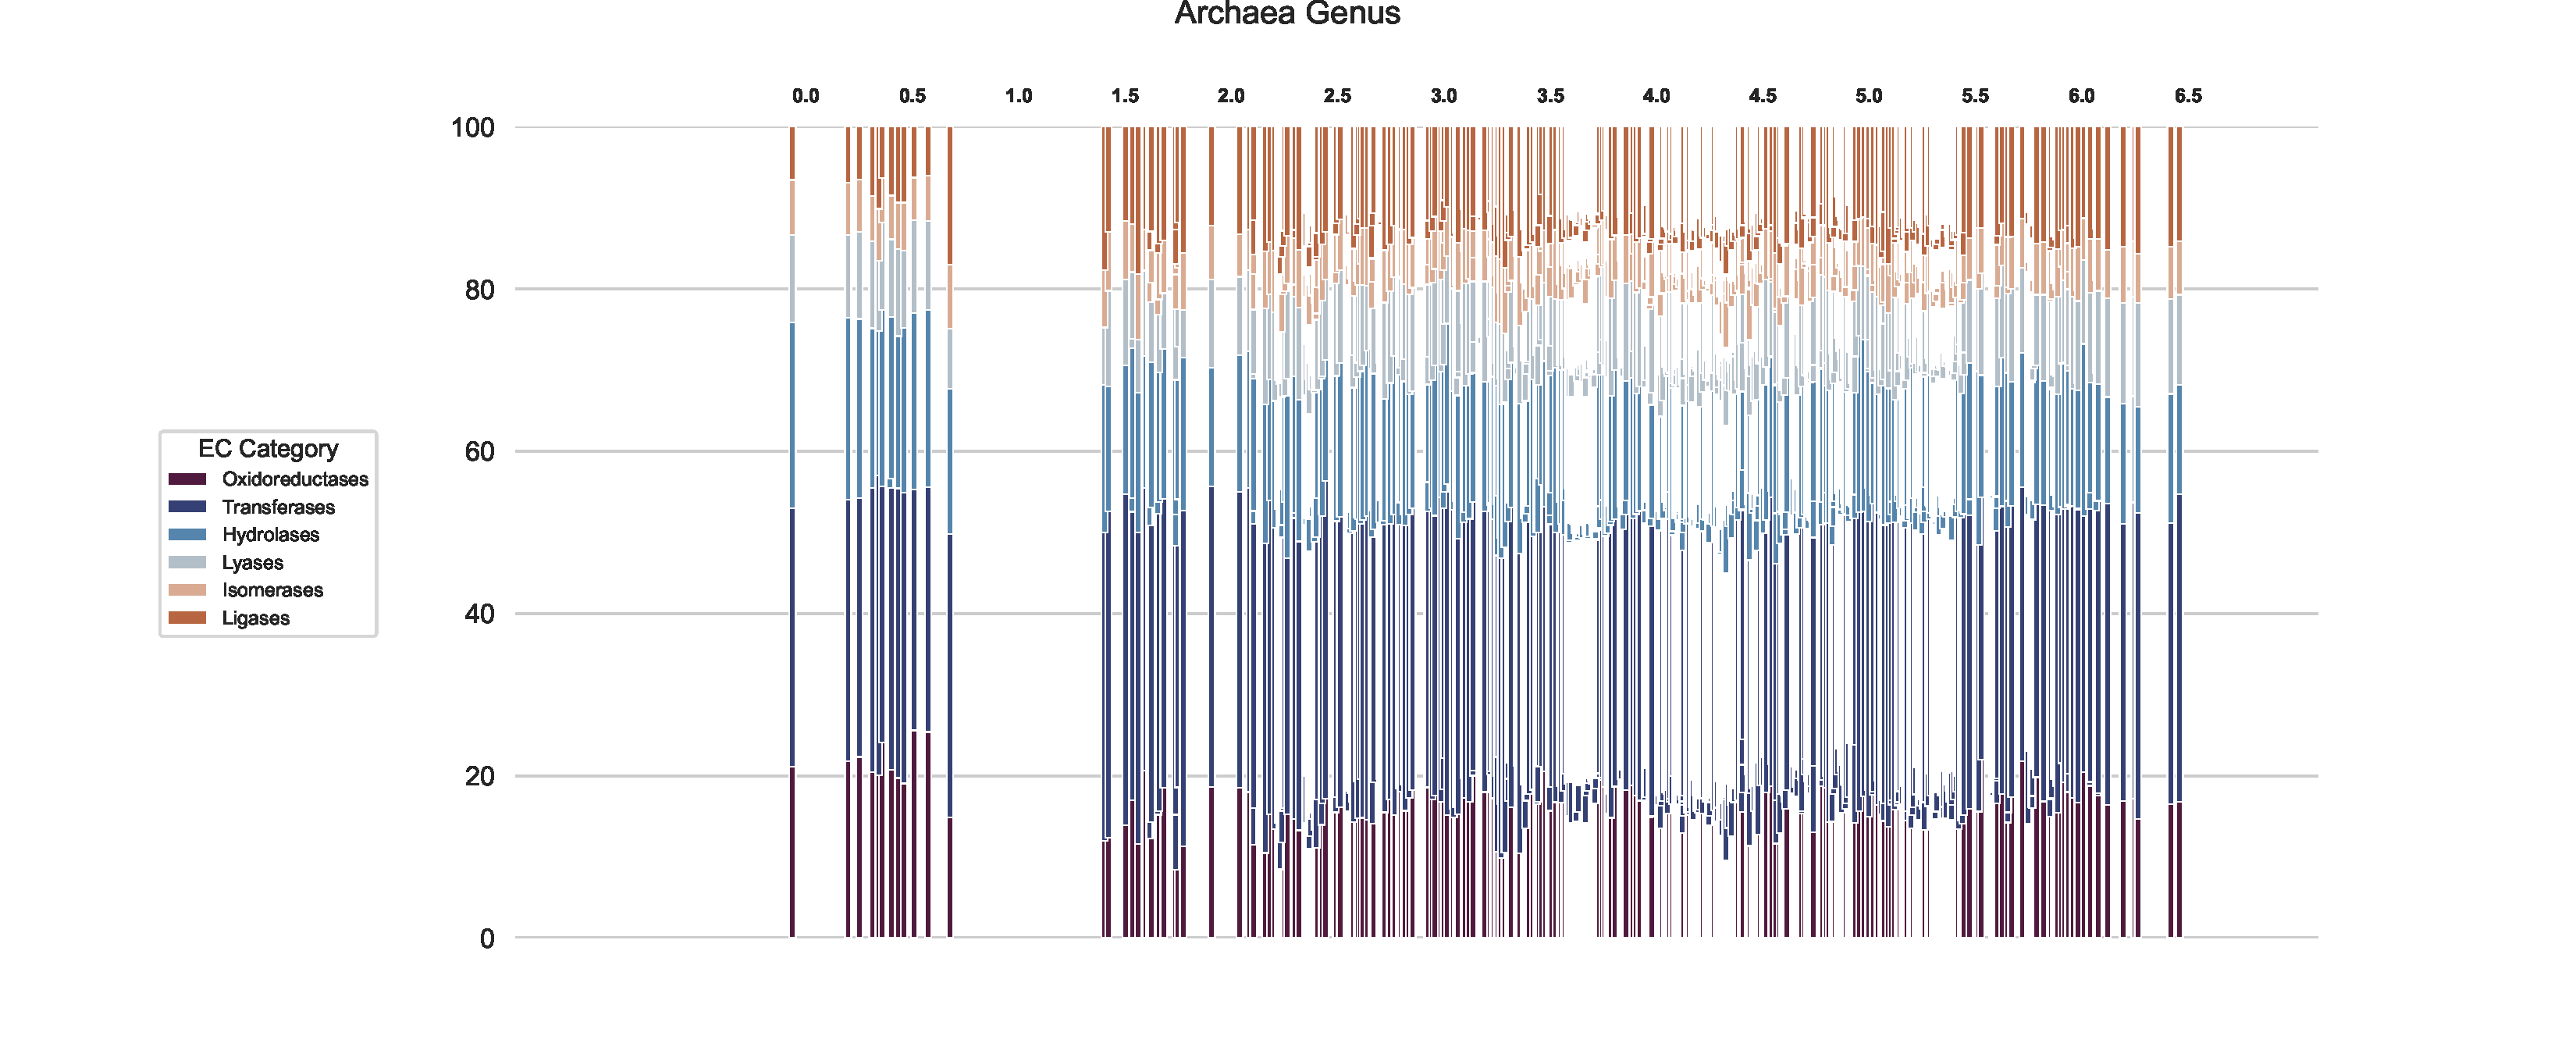
\includegraphics[width=0.95\textwidth]{ridgeplots/gen4arc_barplot.pdf}
    \caption[]{Evolution of individual enzyme categories for the genus-level archaea dataset. The ridgeplot displays the distribution of each category as a function of distance from the tree root, with the last axis presenting the species distribution, while the barplot the relative abundance of each category at that particular distance as a stacked barplot.}
    \label{barplot_gen4arc}
\end{figure}


\newpage
\subsection*{A3. Expansion Scope Size as a Function of Distance to Root}
\textbf{For every taxonomic level dataset, per seed set.}

\begin{figure}[H]
    \centering
    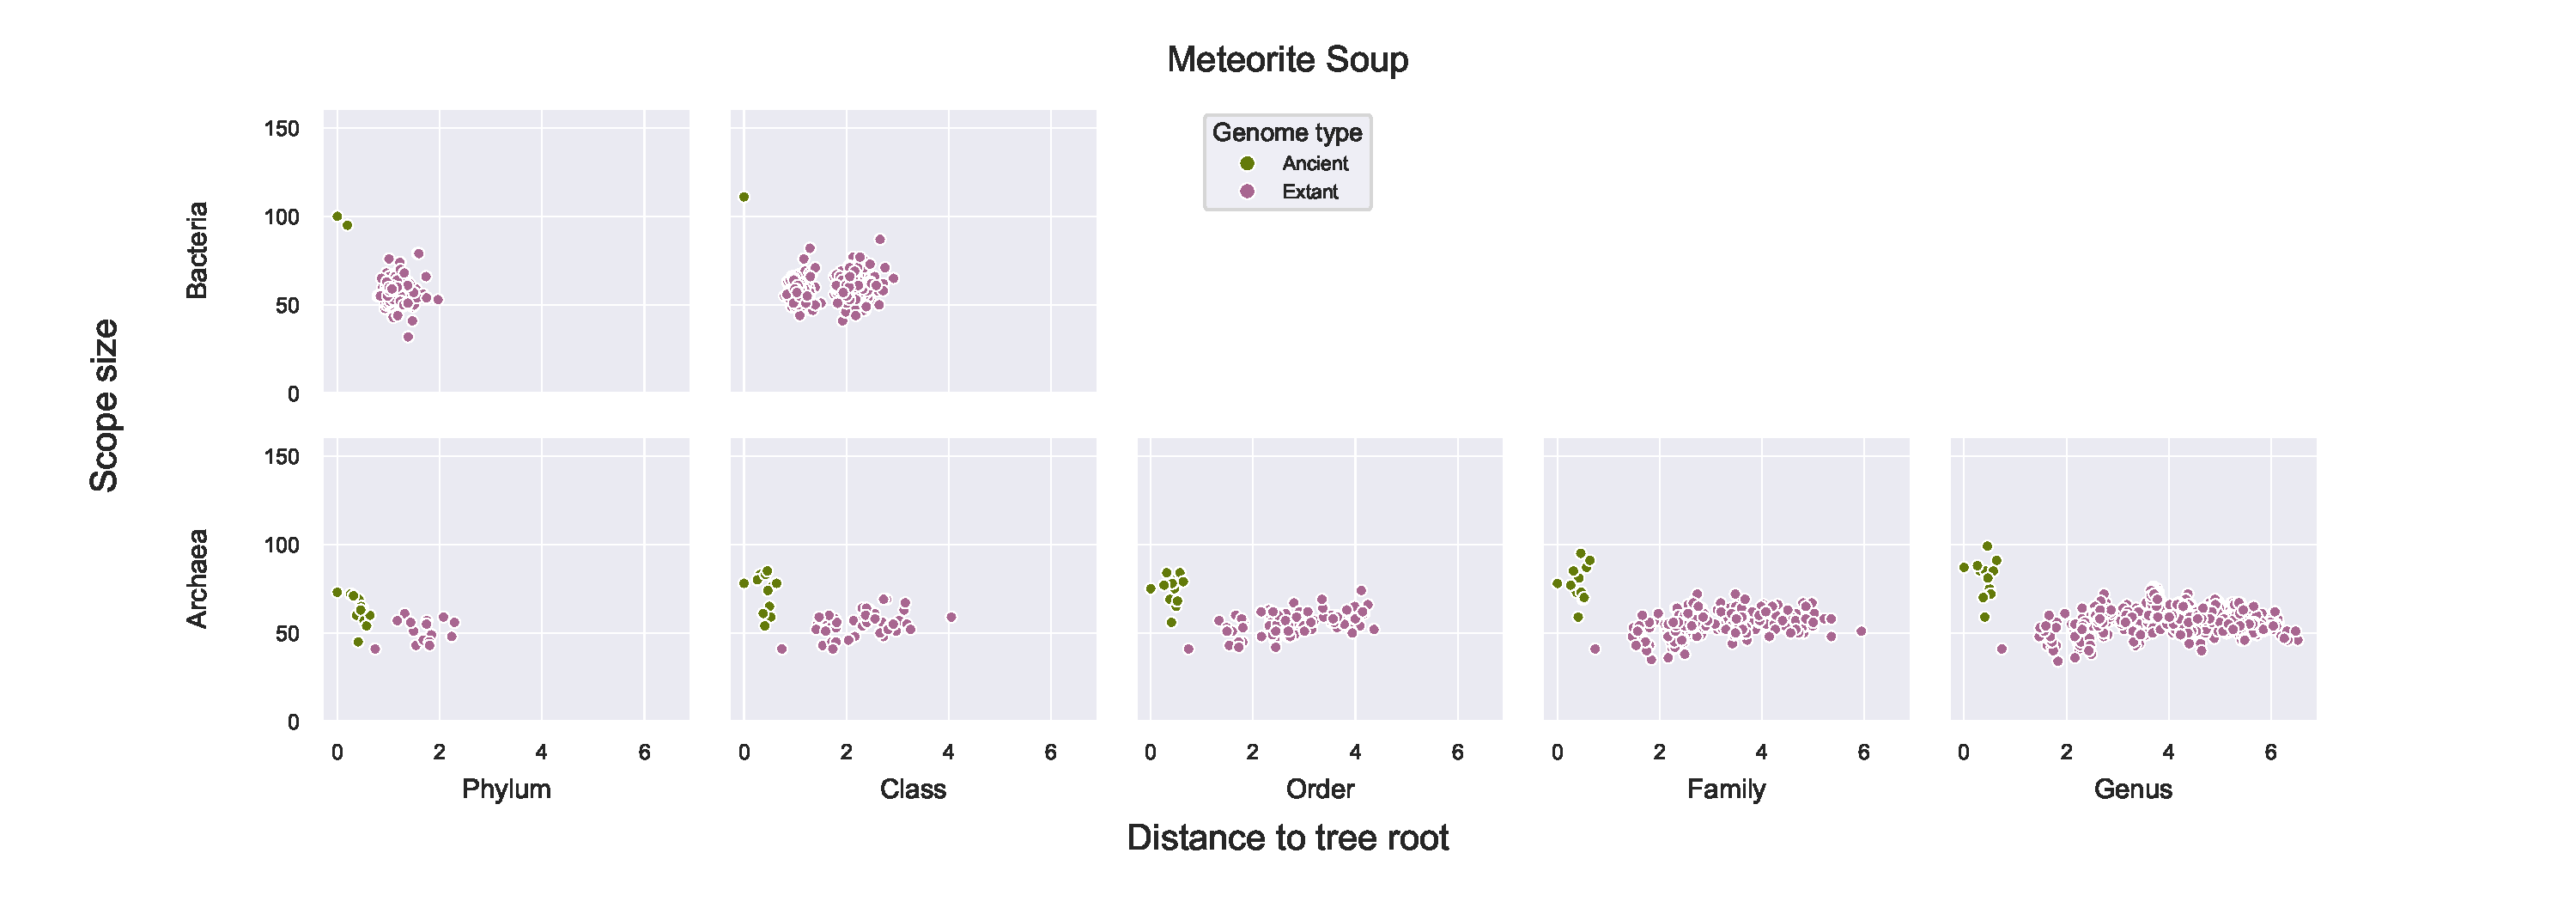
\includegraphics[width=0.95\textwidth]{scopesize_vs_disttoroot/gfm_ss_rootdist}
    \caption{Goldford + meteoritic soup}
    \label{gfm_scopesize}
\end{figure}   

\begin{figure}[H]
    \centering
    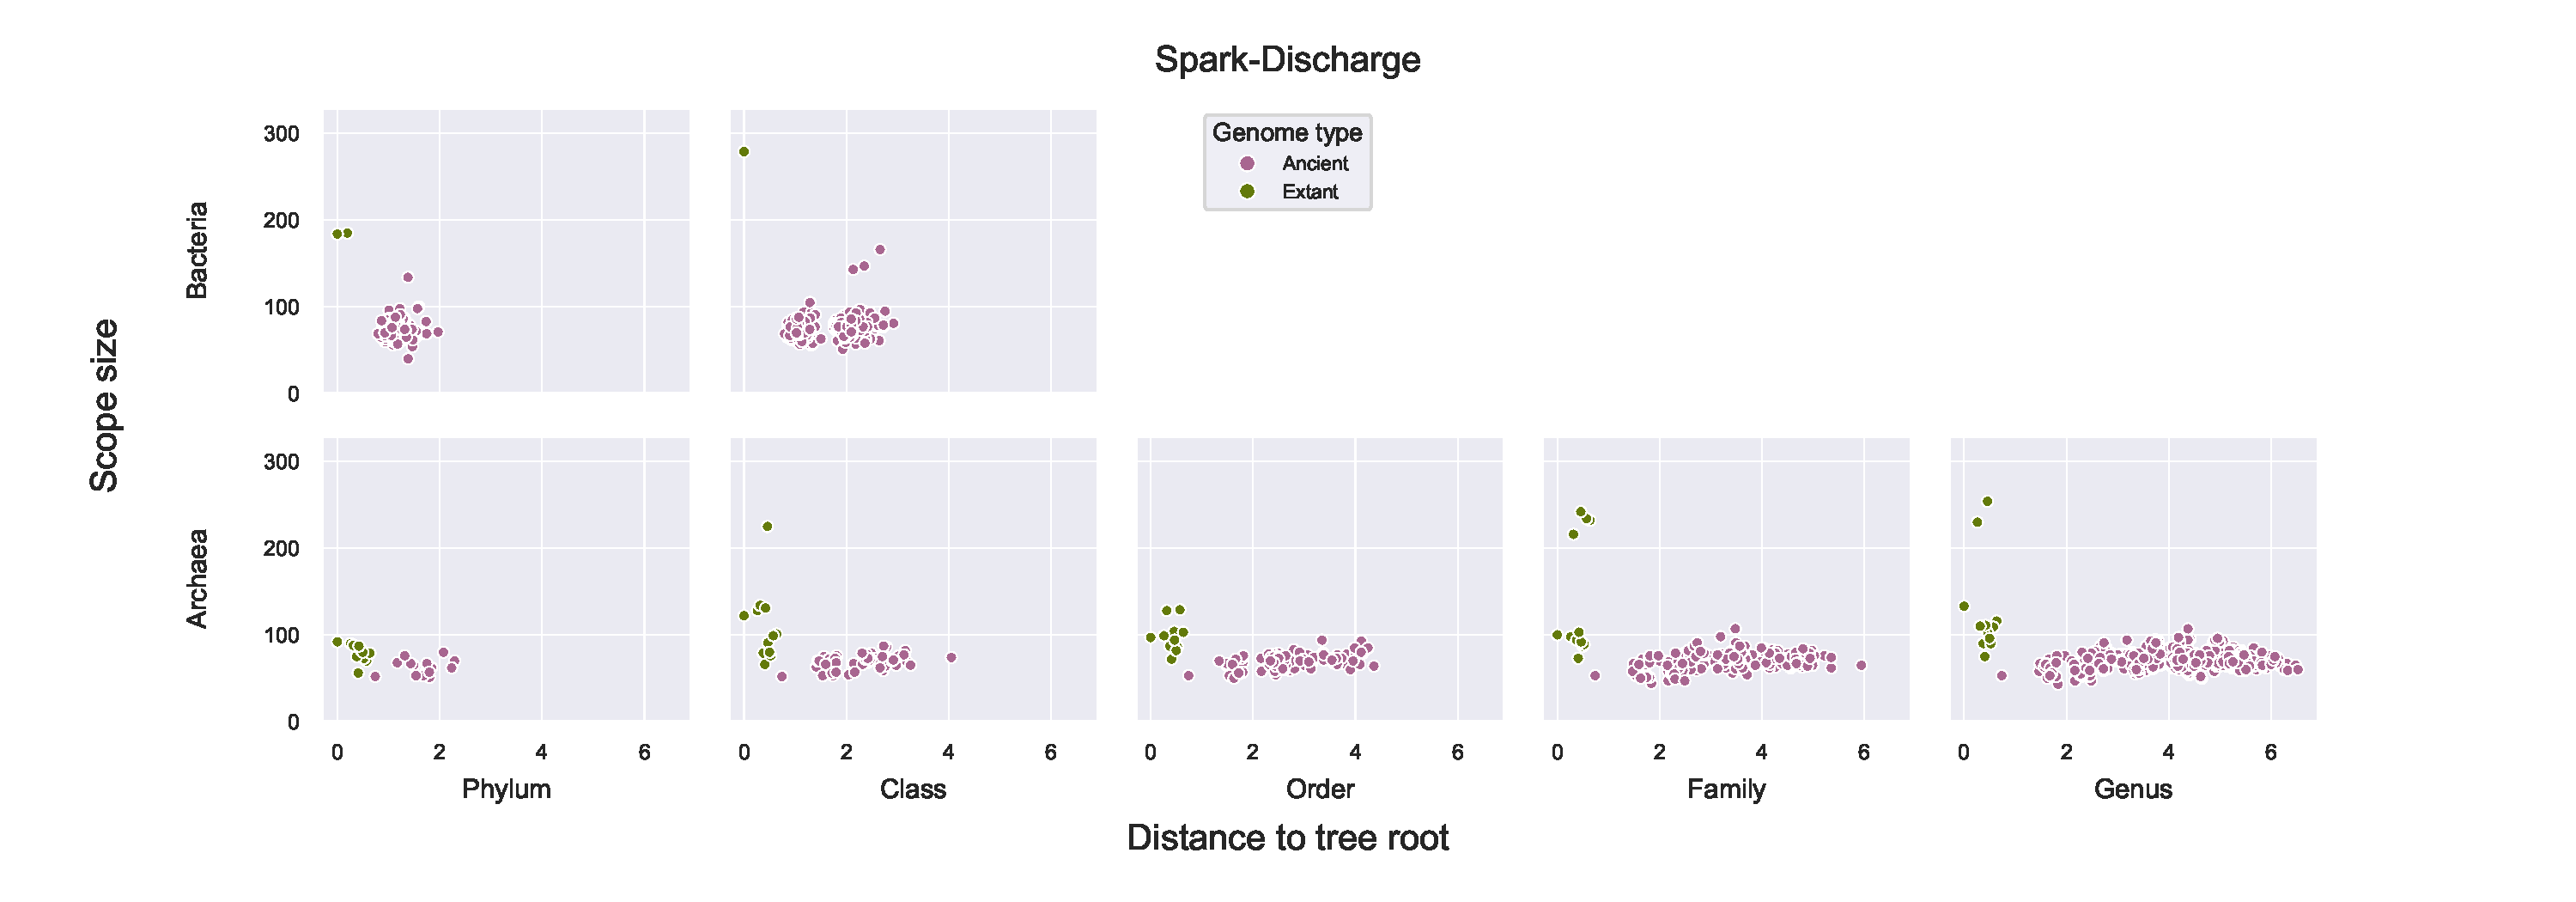
\includegraphics[width=0.95\textwidth]{scopesize_vs_disttoroot/gfsd_ss_rootdist.pdf}
    \caption{Goldford + spark-discharge}
    \label{gfsd_scopesize}
\end{figure}   

\begin{figure}[H]
    \centering
    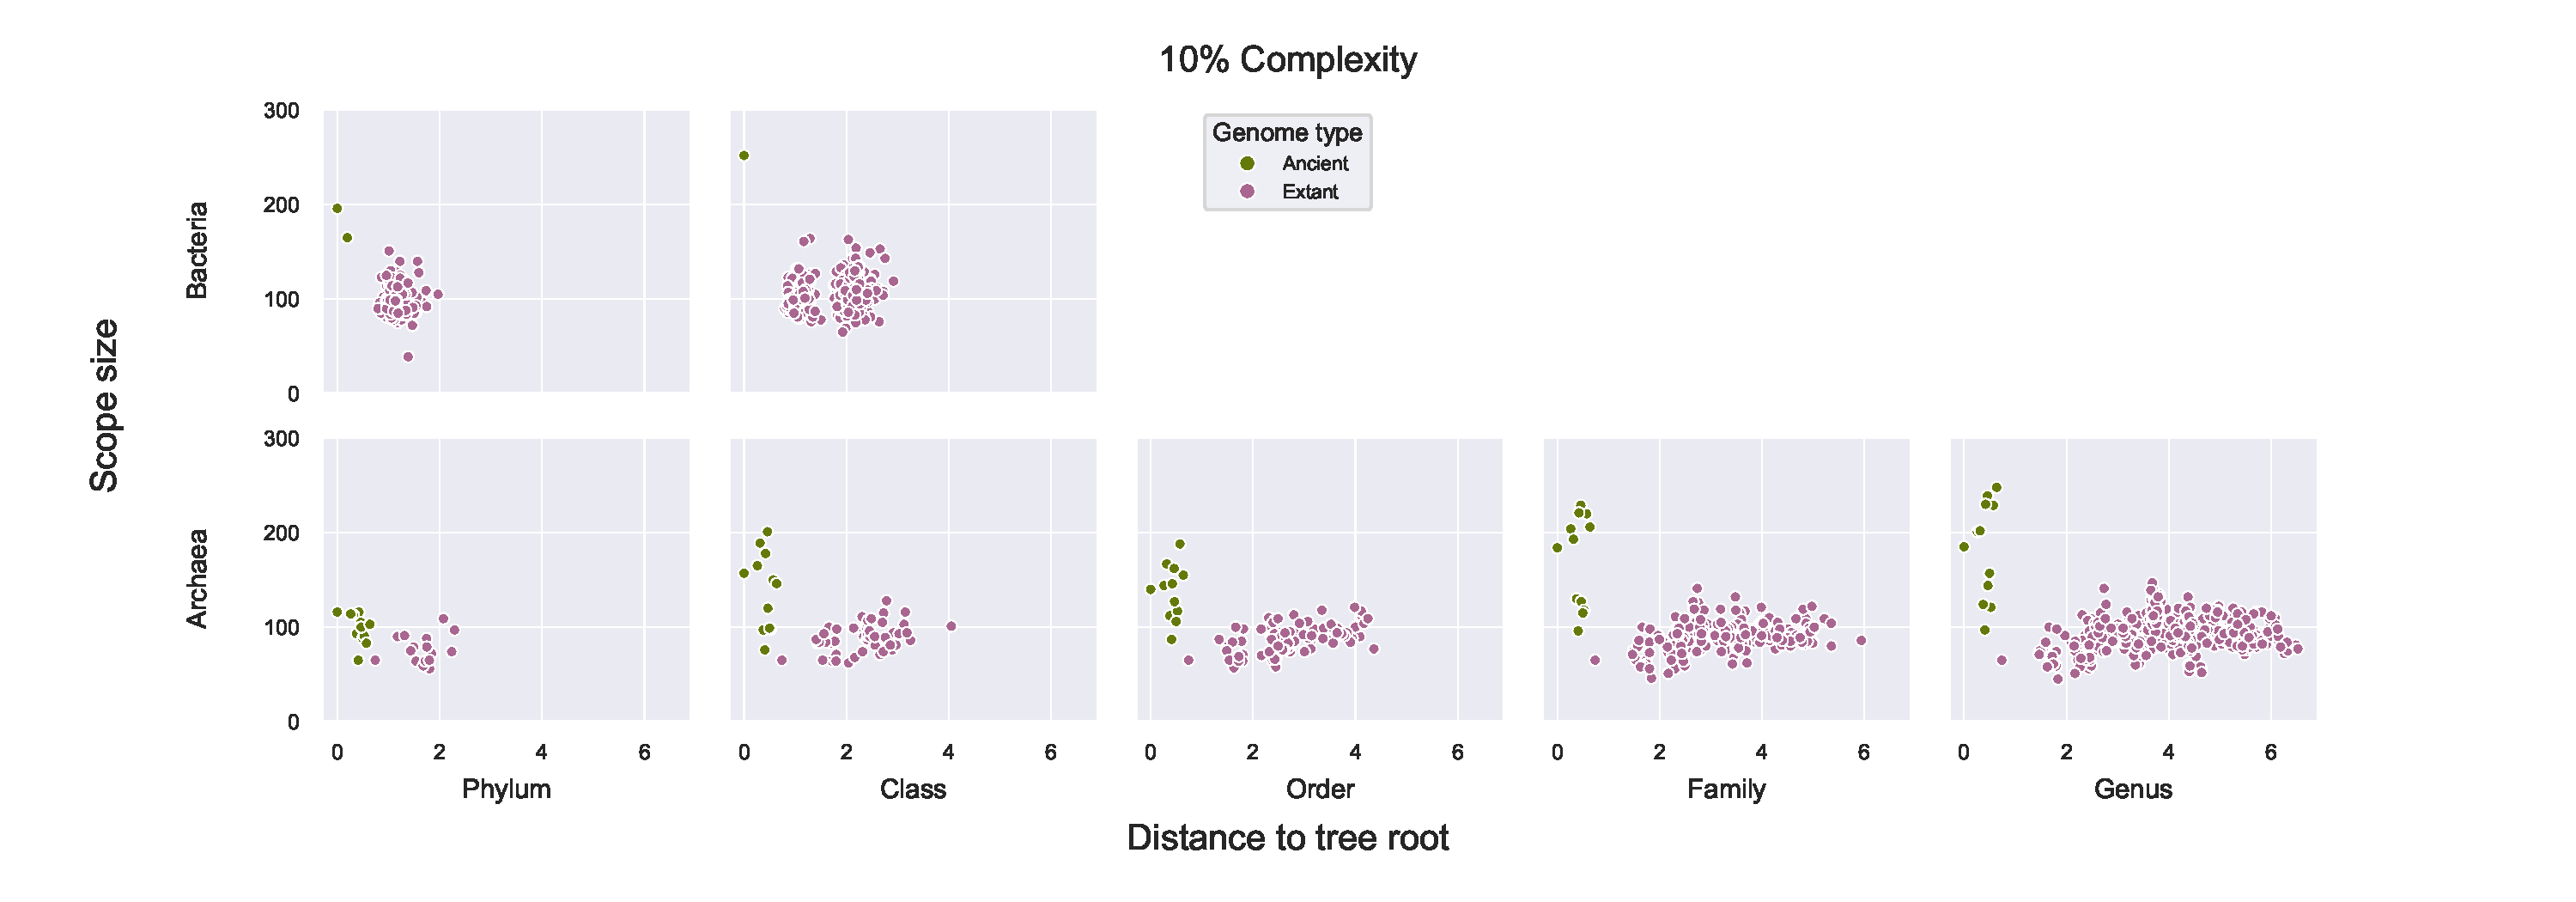
\includegraphics[width=0.95\textwidth]{scopesize_vs_disttoroot/0.1_ss_rootdist.pdf}
    \caption{10\% complexity}
    \label{0.1_scopesize}
\end{figure}   

\begin{figure}[H]
    \centering
    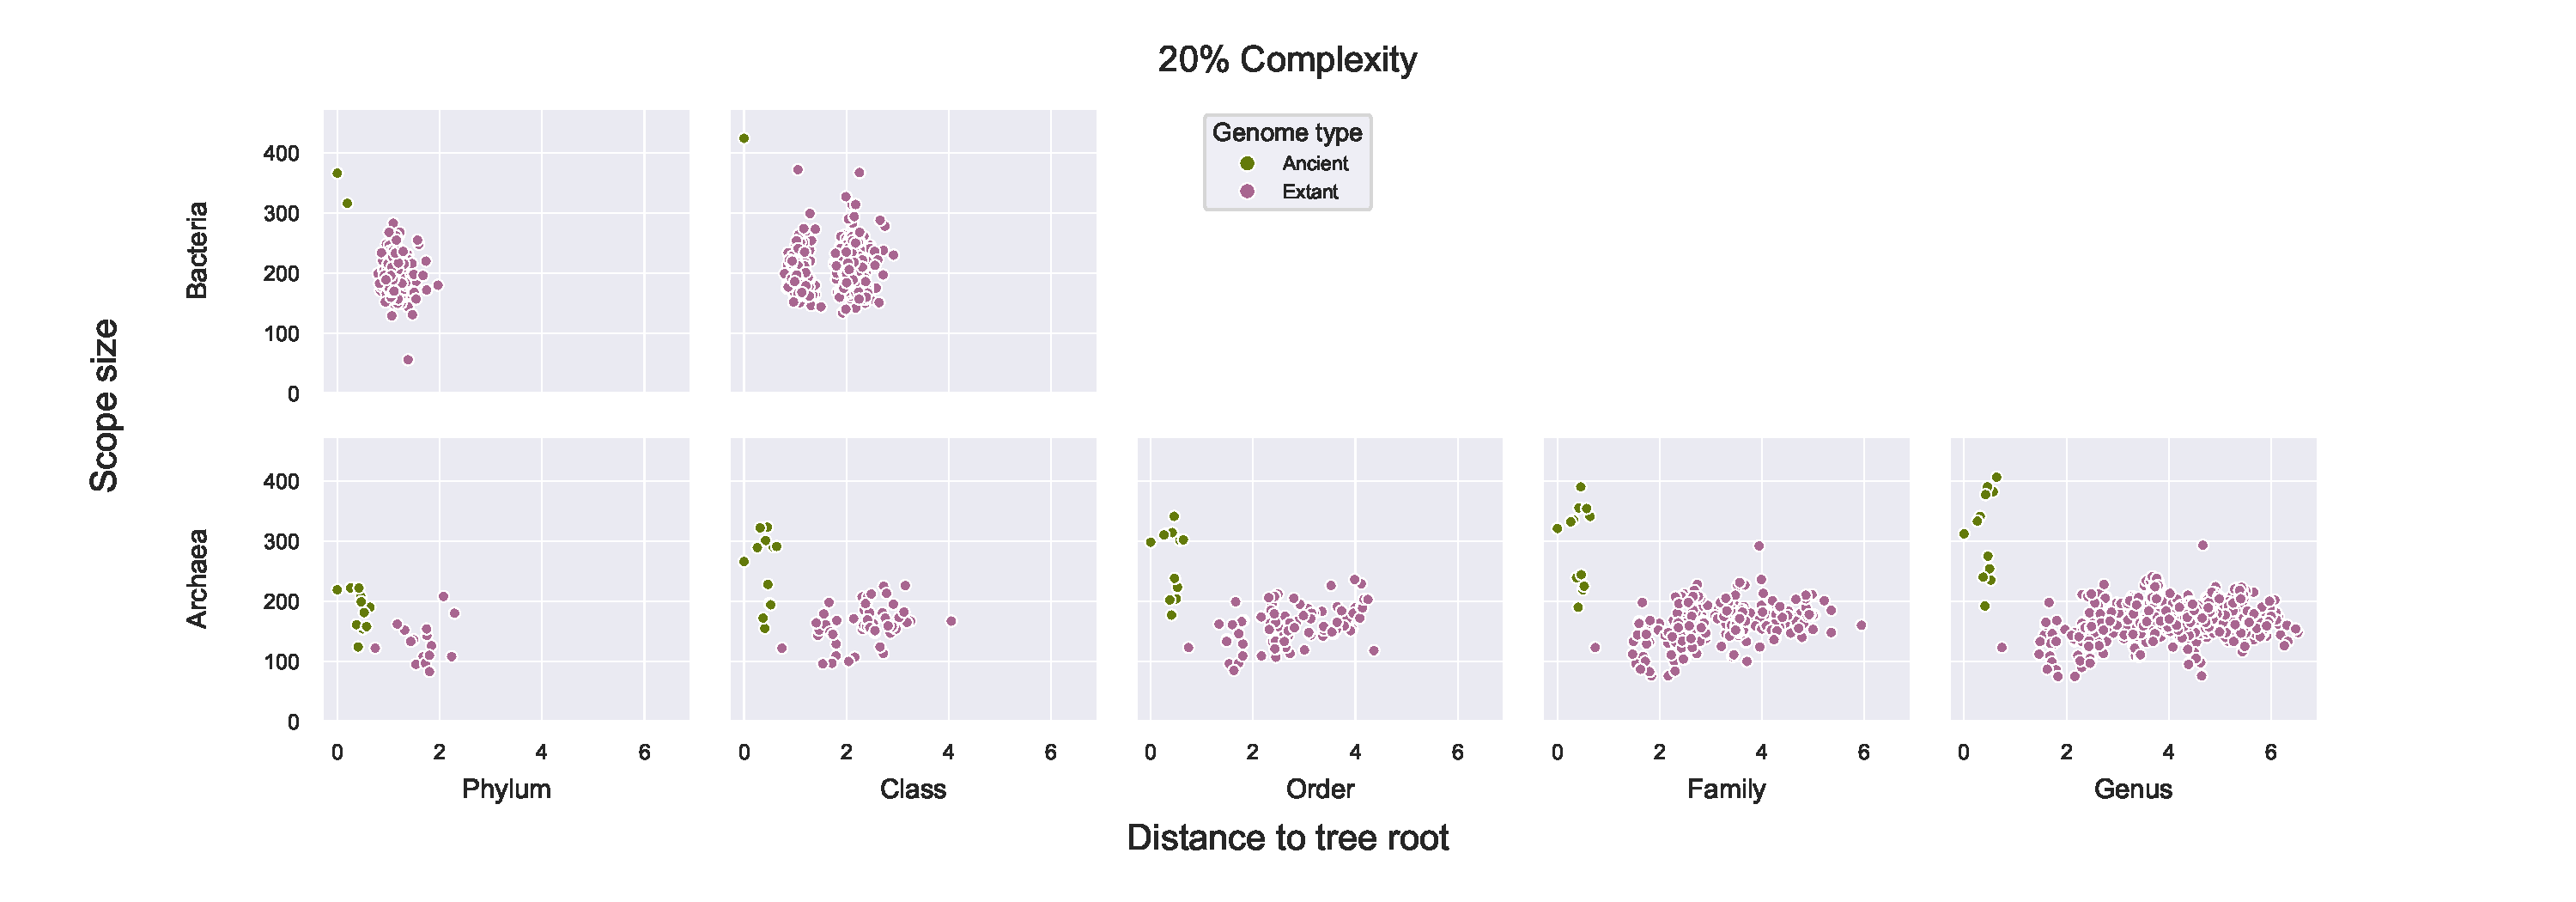
\includegraphics[width=0.95\textwidth]{scopesize_vs_disttoroot/0.2_ss_rootdist.pdf}
    \caption{20\% complexity}
    \label{0.2_scopesize}
\end{figure}   

\begin{figure}[H]
    \centering
    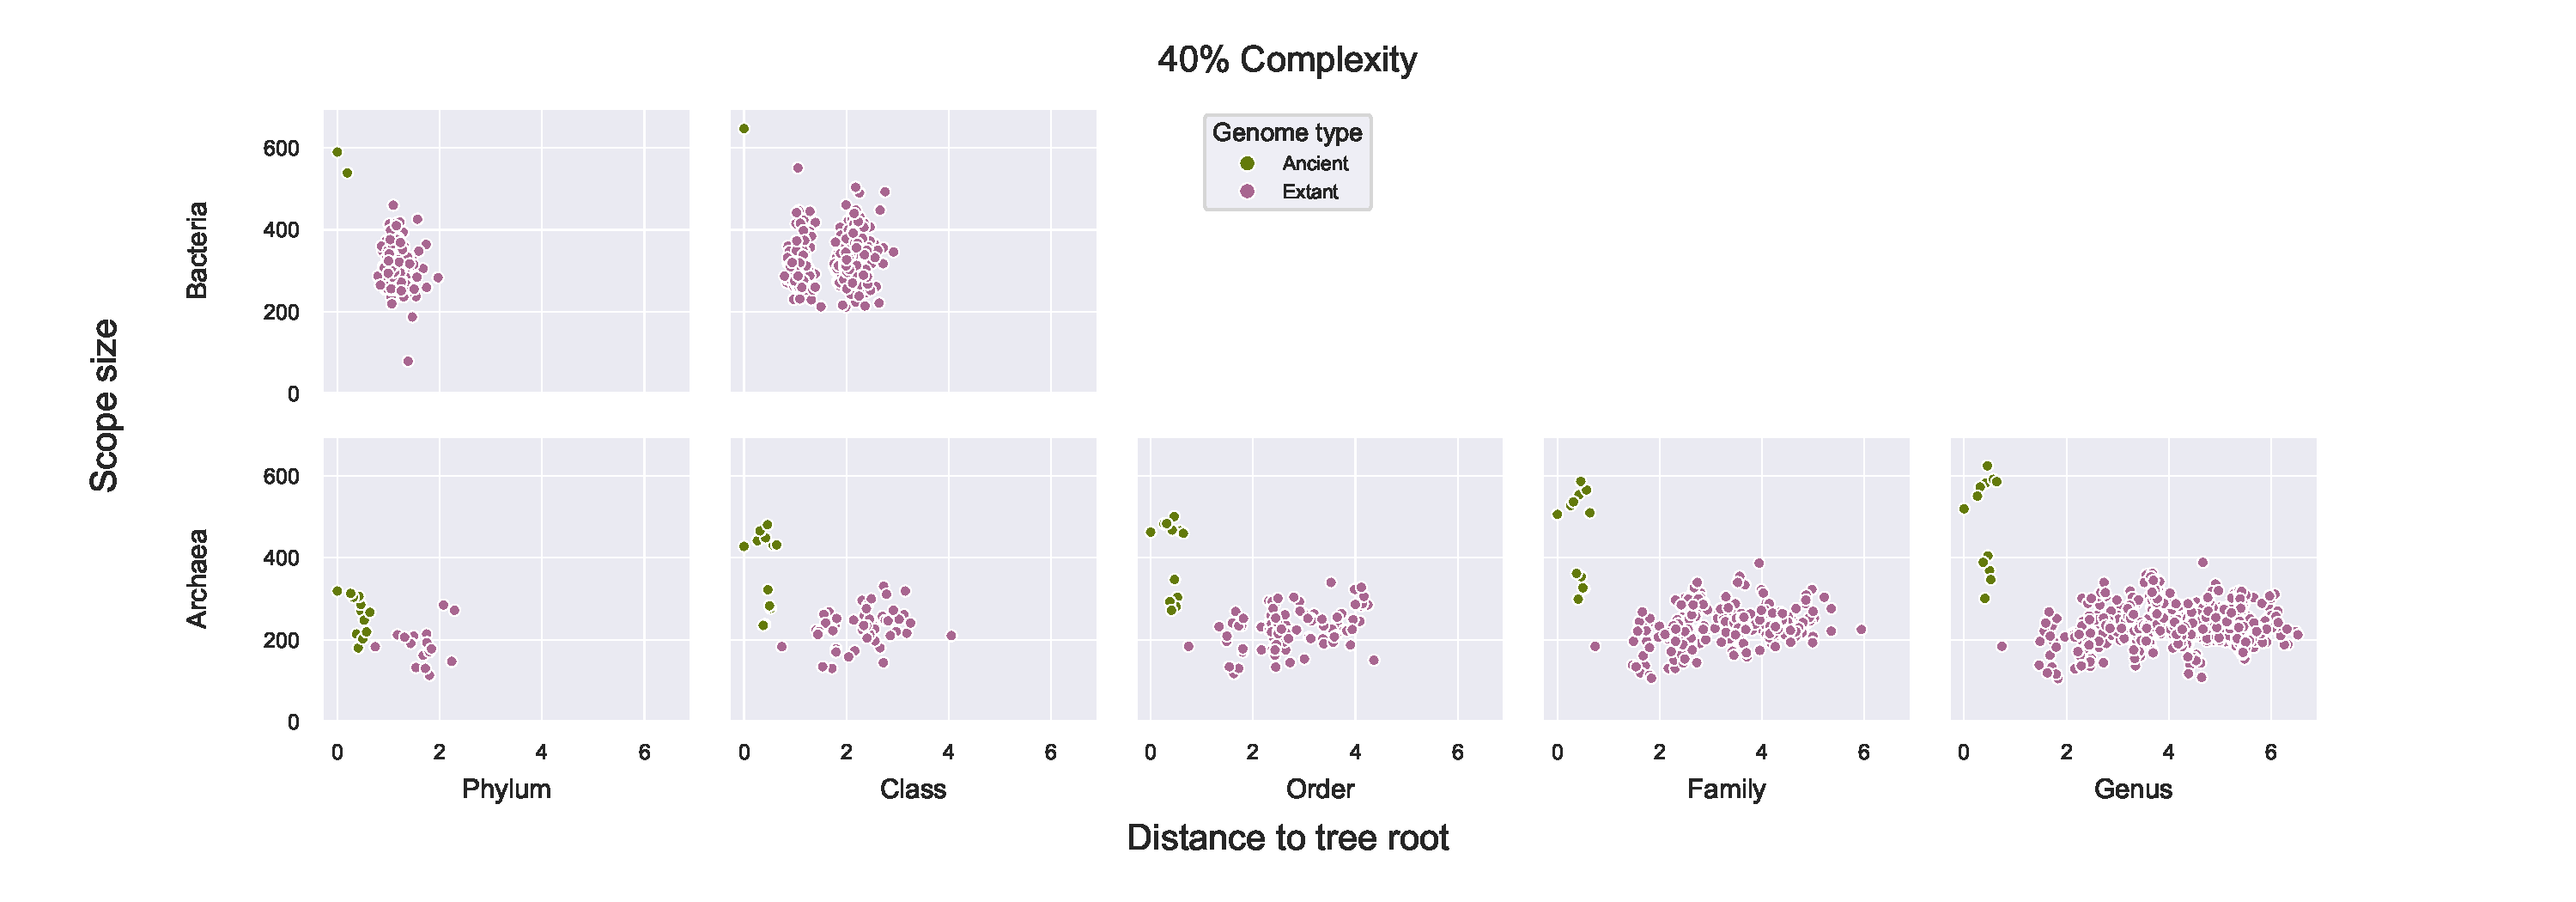
\includegraphics[width=0.95\textwidth]{scopesize_vs_disttoroot/0.4_ss_rootdist.pdf}
    \caption{40\% complexity}
    \label{0.4_scopesize}
\end{figure}   

\begin{figure}[H]
    \centering
    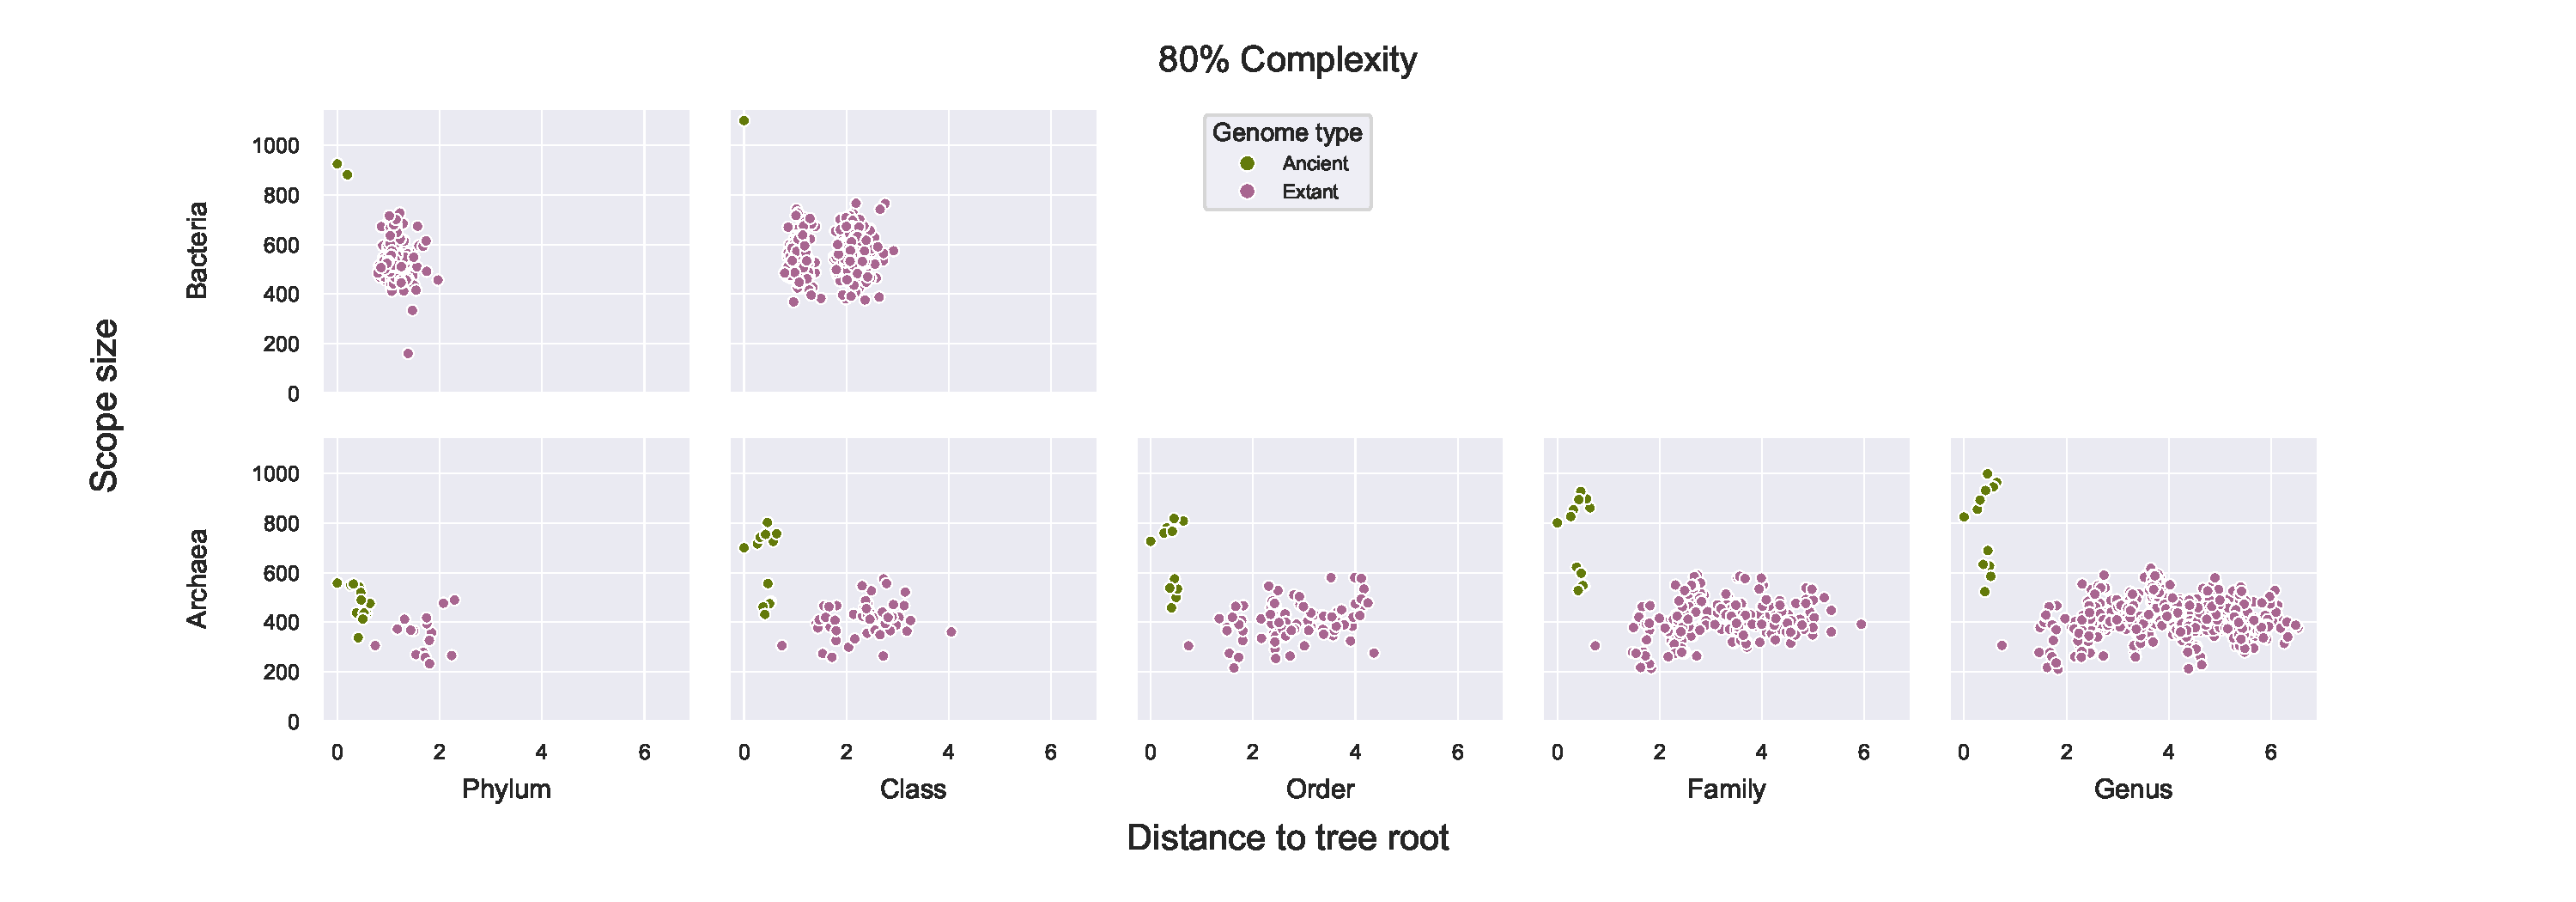
\includegraphics[width=0.95\textwidth]{scopesize_vs_disttoroot/0.8_ss_rootdist.pdf}
    \caption{80\% complexity}
    \label{0.8_scopesize}
\end{figure}   

\begin{figure}[H]
    \centering
    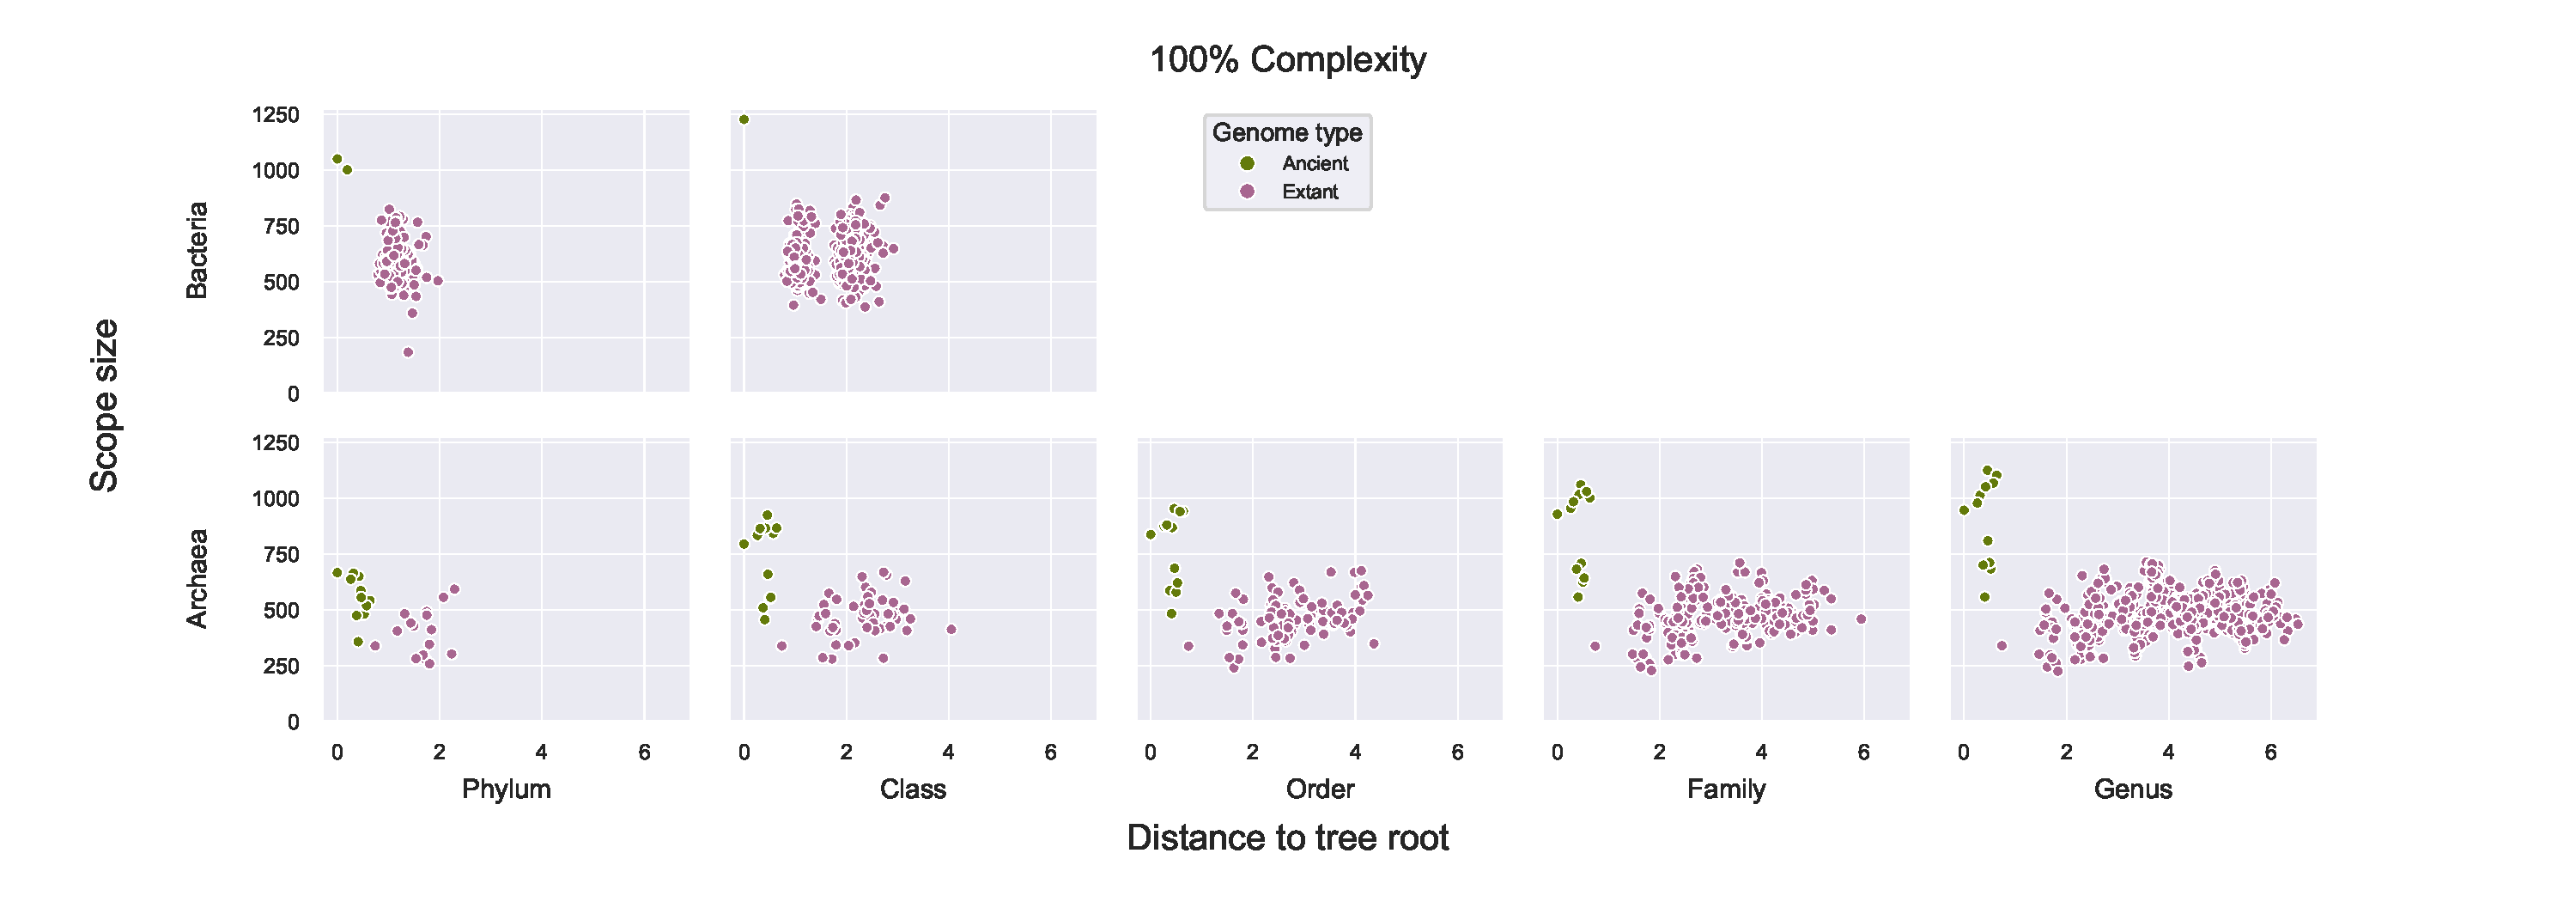
\includegraphics[width=0.95\textwidth]{scopesize_vs_disttoroot/1_ss_rootdist.pdf}
    \caption{100\% complexity}
    \label{1_scopesize}
\end{figure}   

\textbf{For every seed set, per taxonomic level dataset.}

\begin{figure}[H]
    \centering
    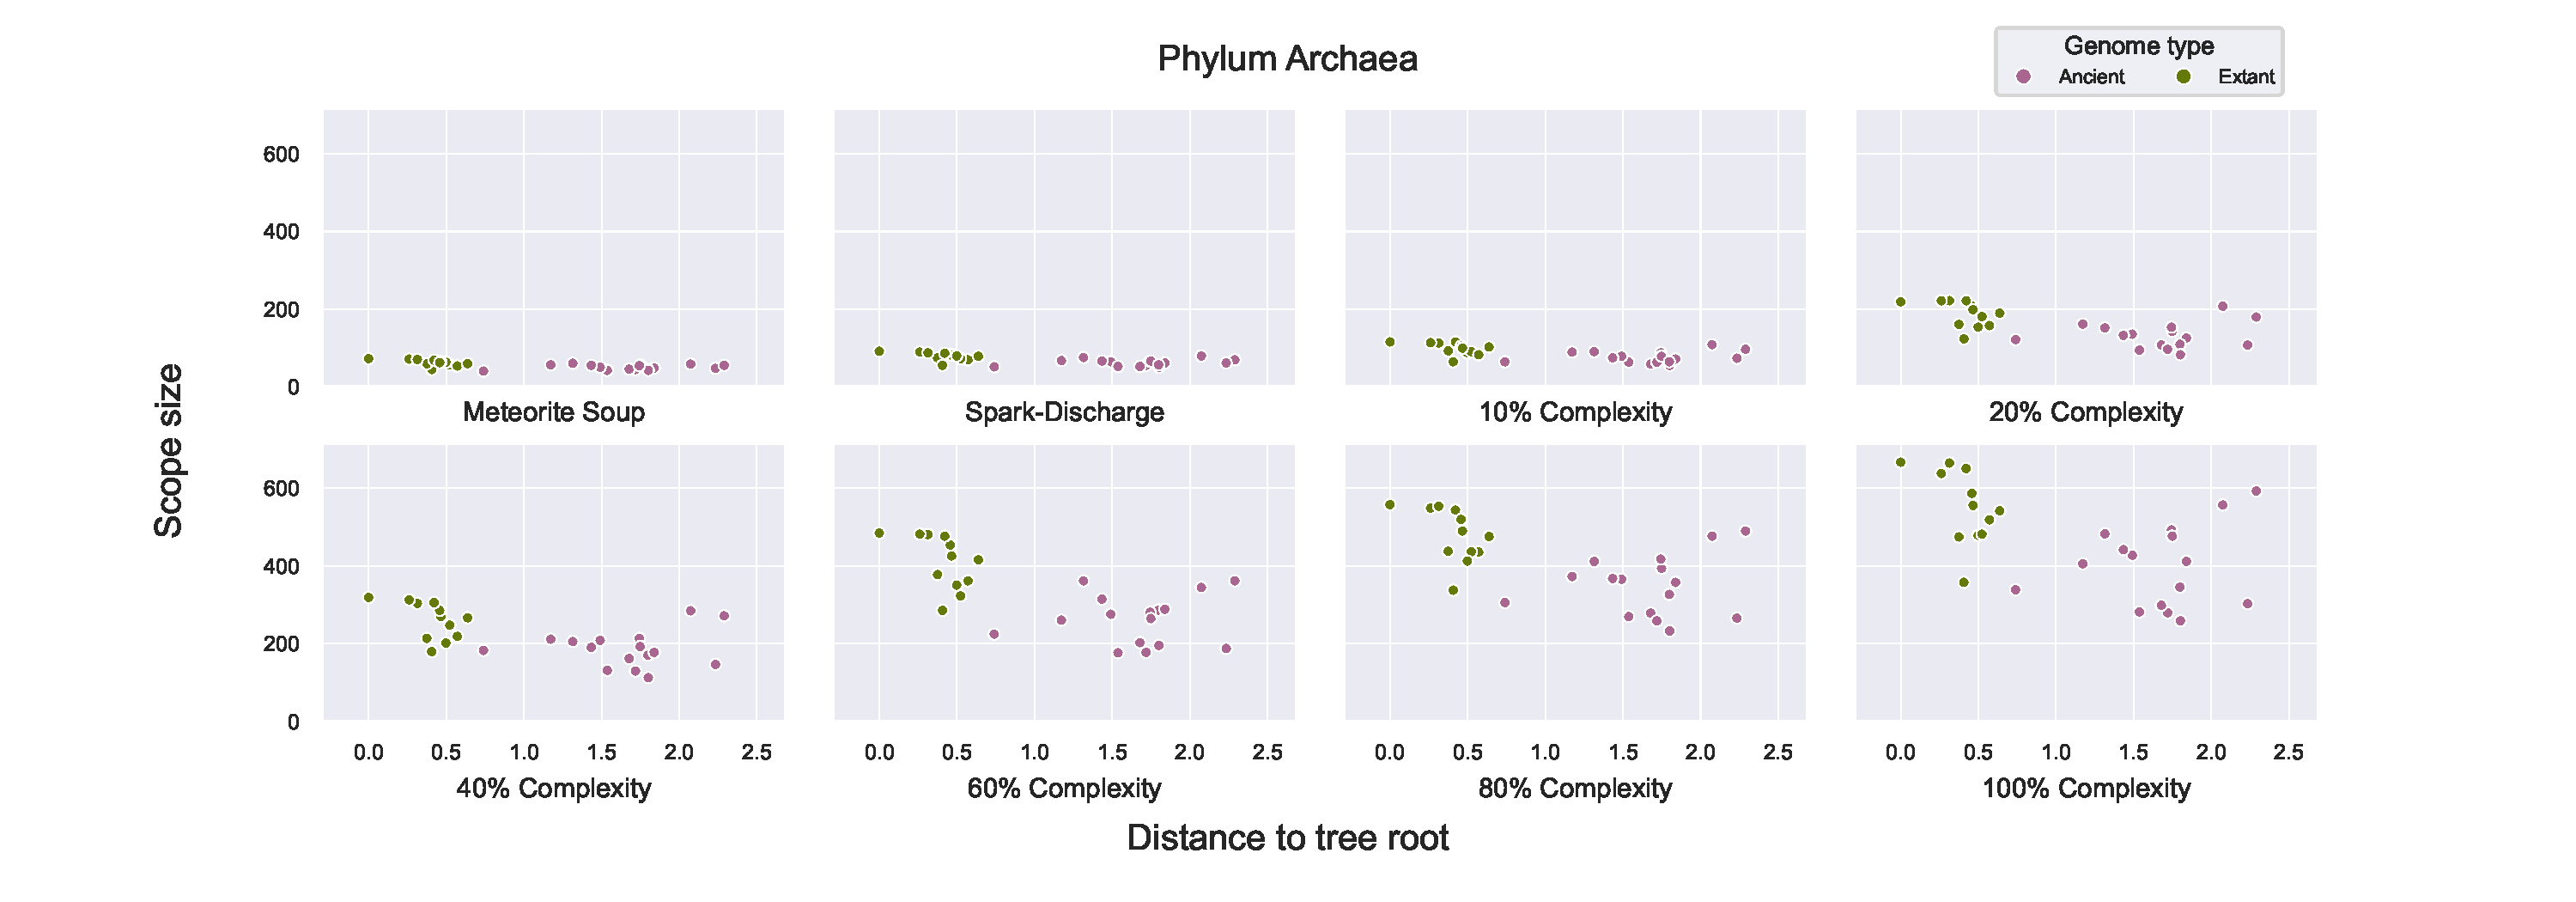
\includegraphics[width=0.95\textwidth]{scopesize_vs_disttoroot/phy4arc_ss_rootdist.pdf}
    \caption{Phylum level archaea}
    \label{phyarc_scopesize}
\end{figure}   

\begin{figure}[H]
    \centering
    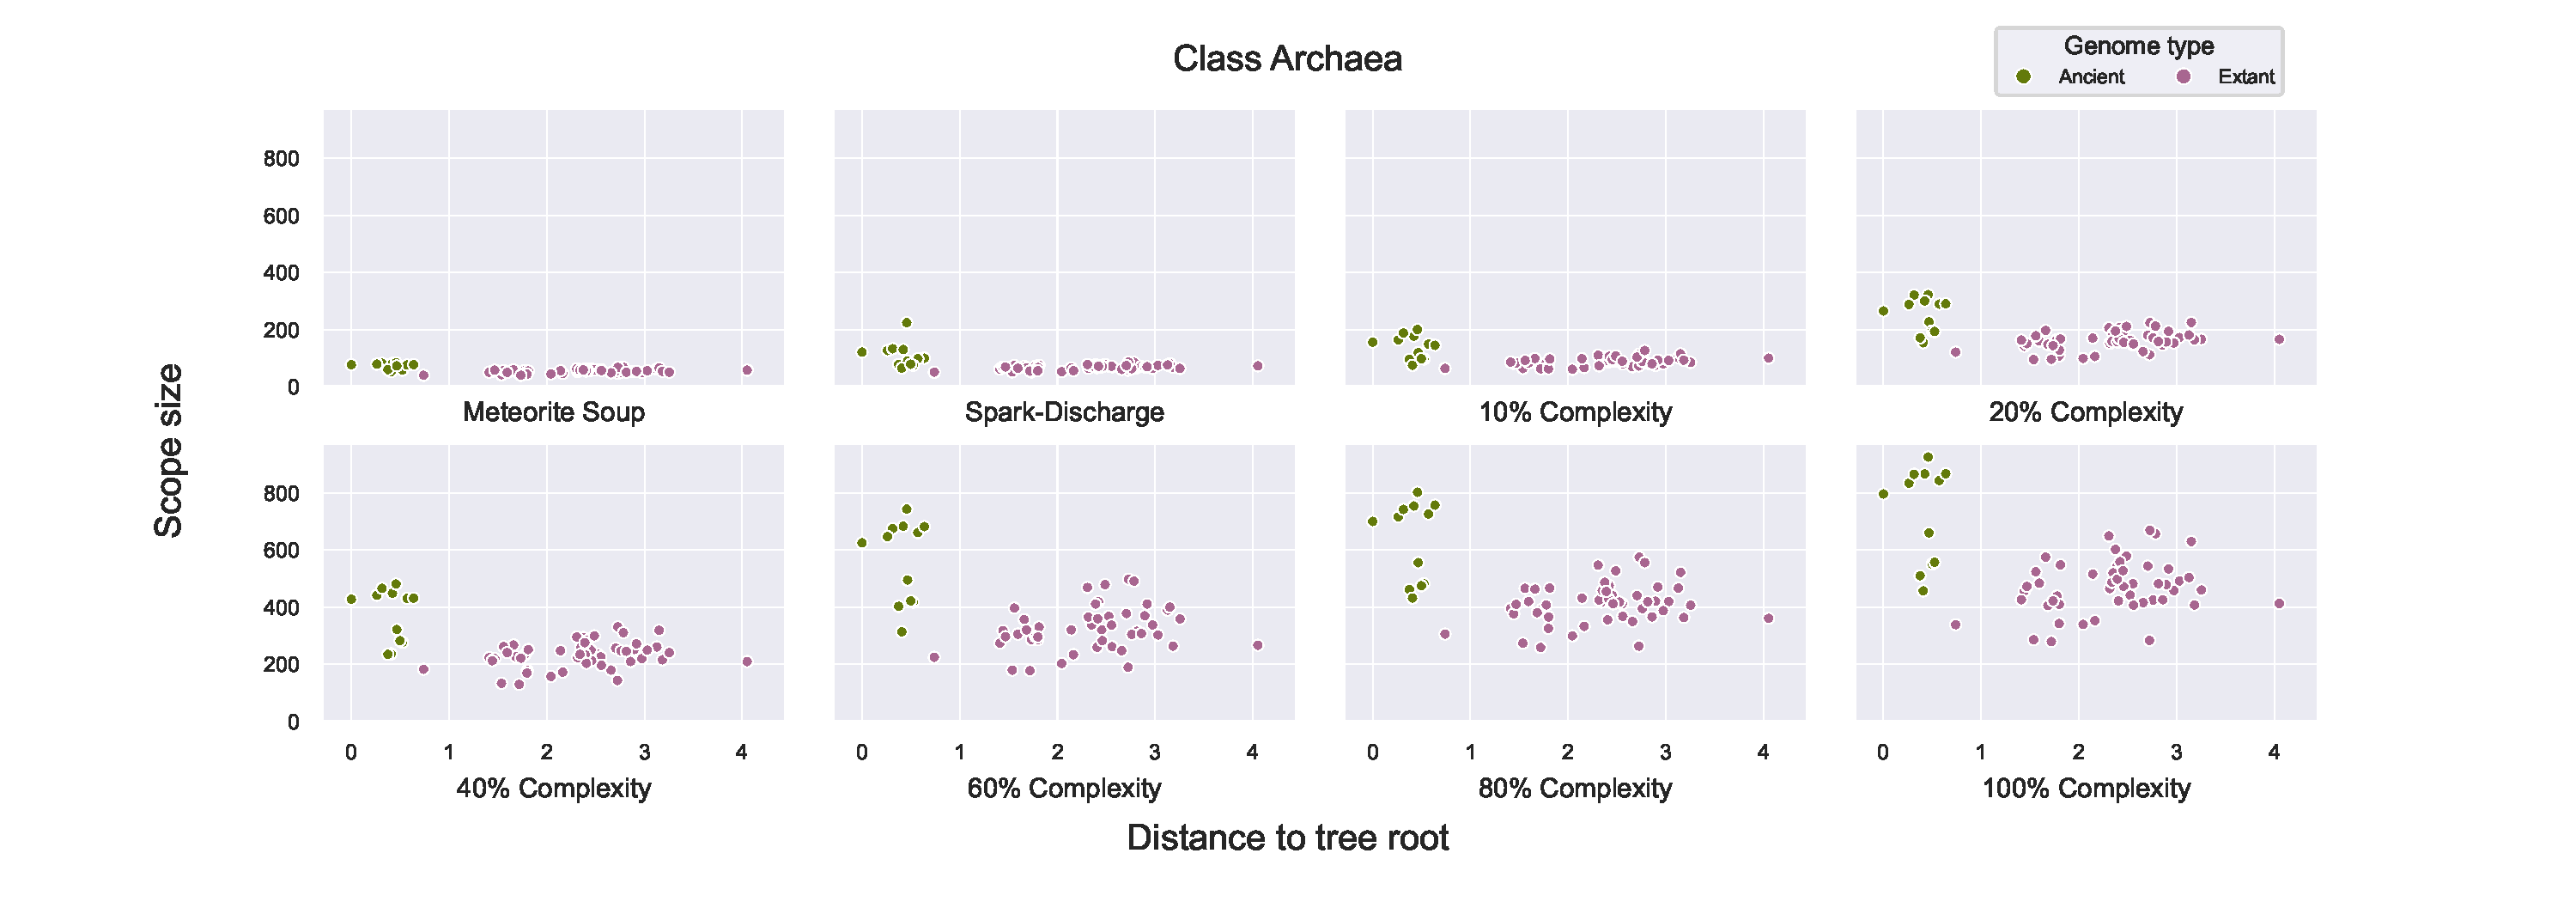
\includegraphics[width=0.95\textwidth]{scopesize_vs_disttoroot/cla4arc_ss_rootdist.pdf}
    \caption{Class level archaea}
    \label{claarc_scopesize}
\end{figure}   

\begin{figure}[H]
    \centering
    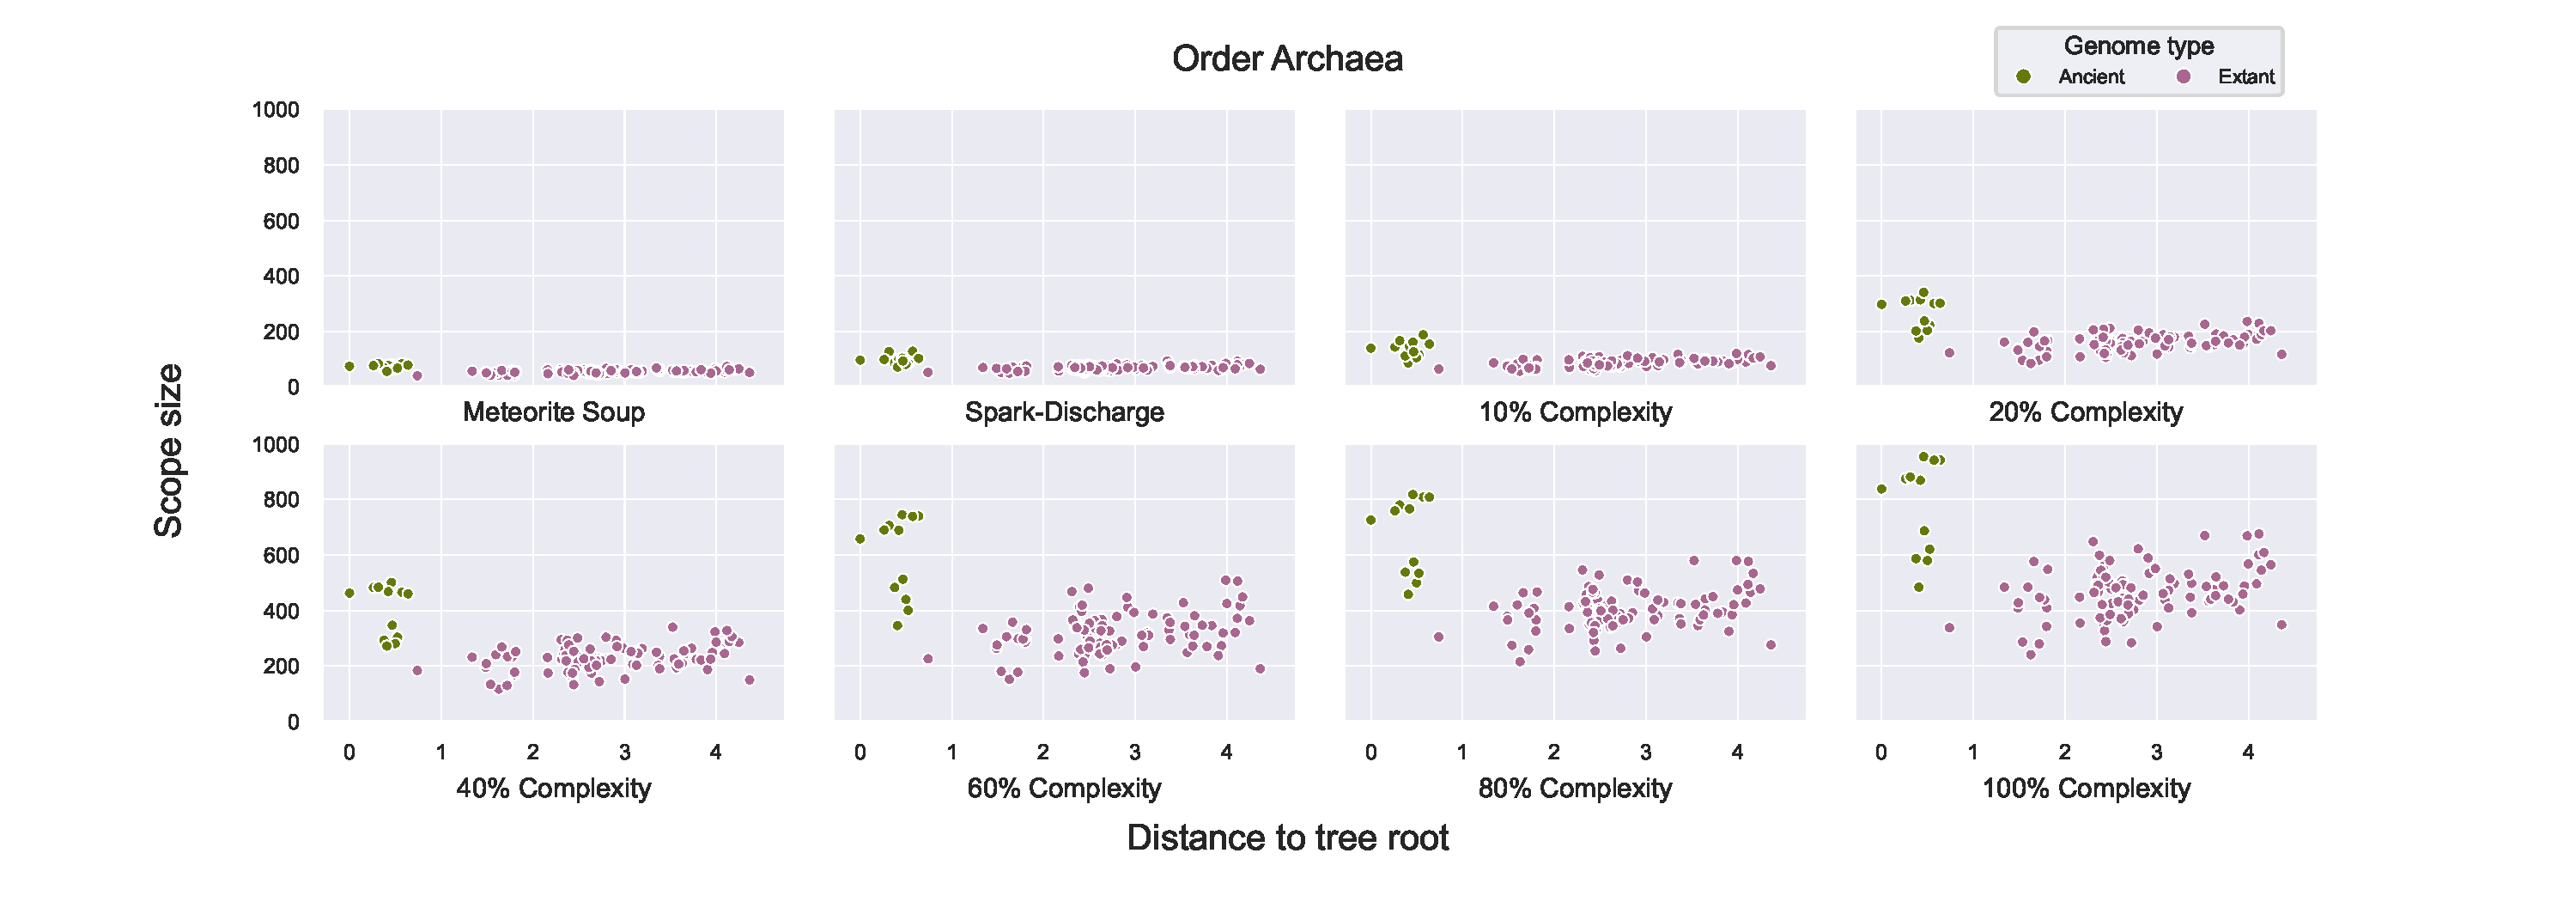
\includegraphics[width=0.95\textwidth]{scopesize_vs_disttoroot/ord4arc_ss_rootdist.pdf}
    \caption{Order level archaea}
    \label{ordarc_scopesize}
\end{figure}   

\begin{figure}[H]
    \centering
    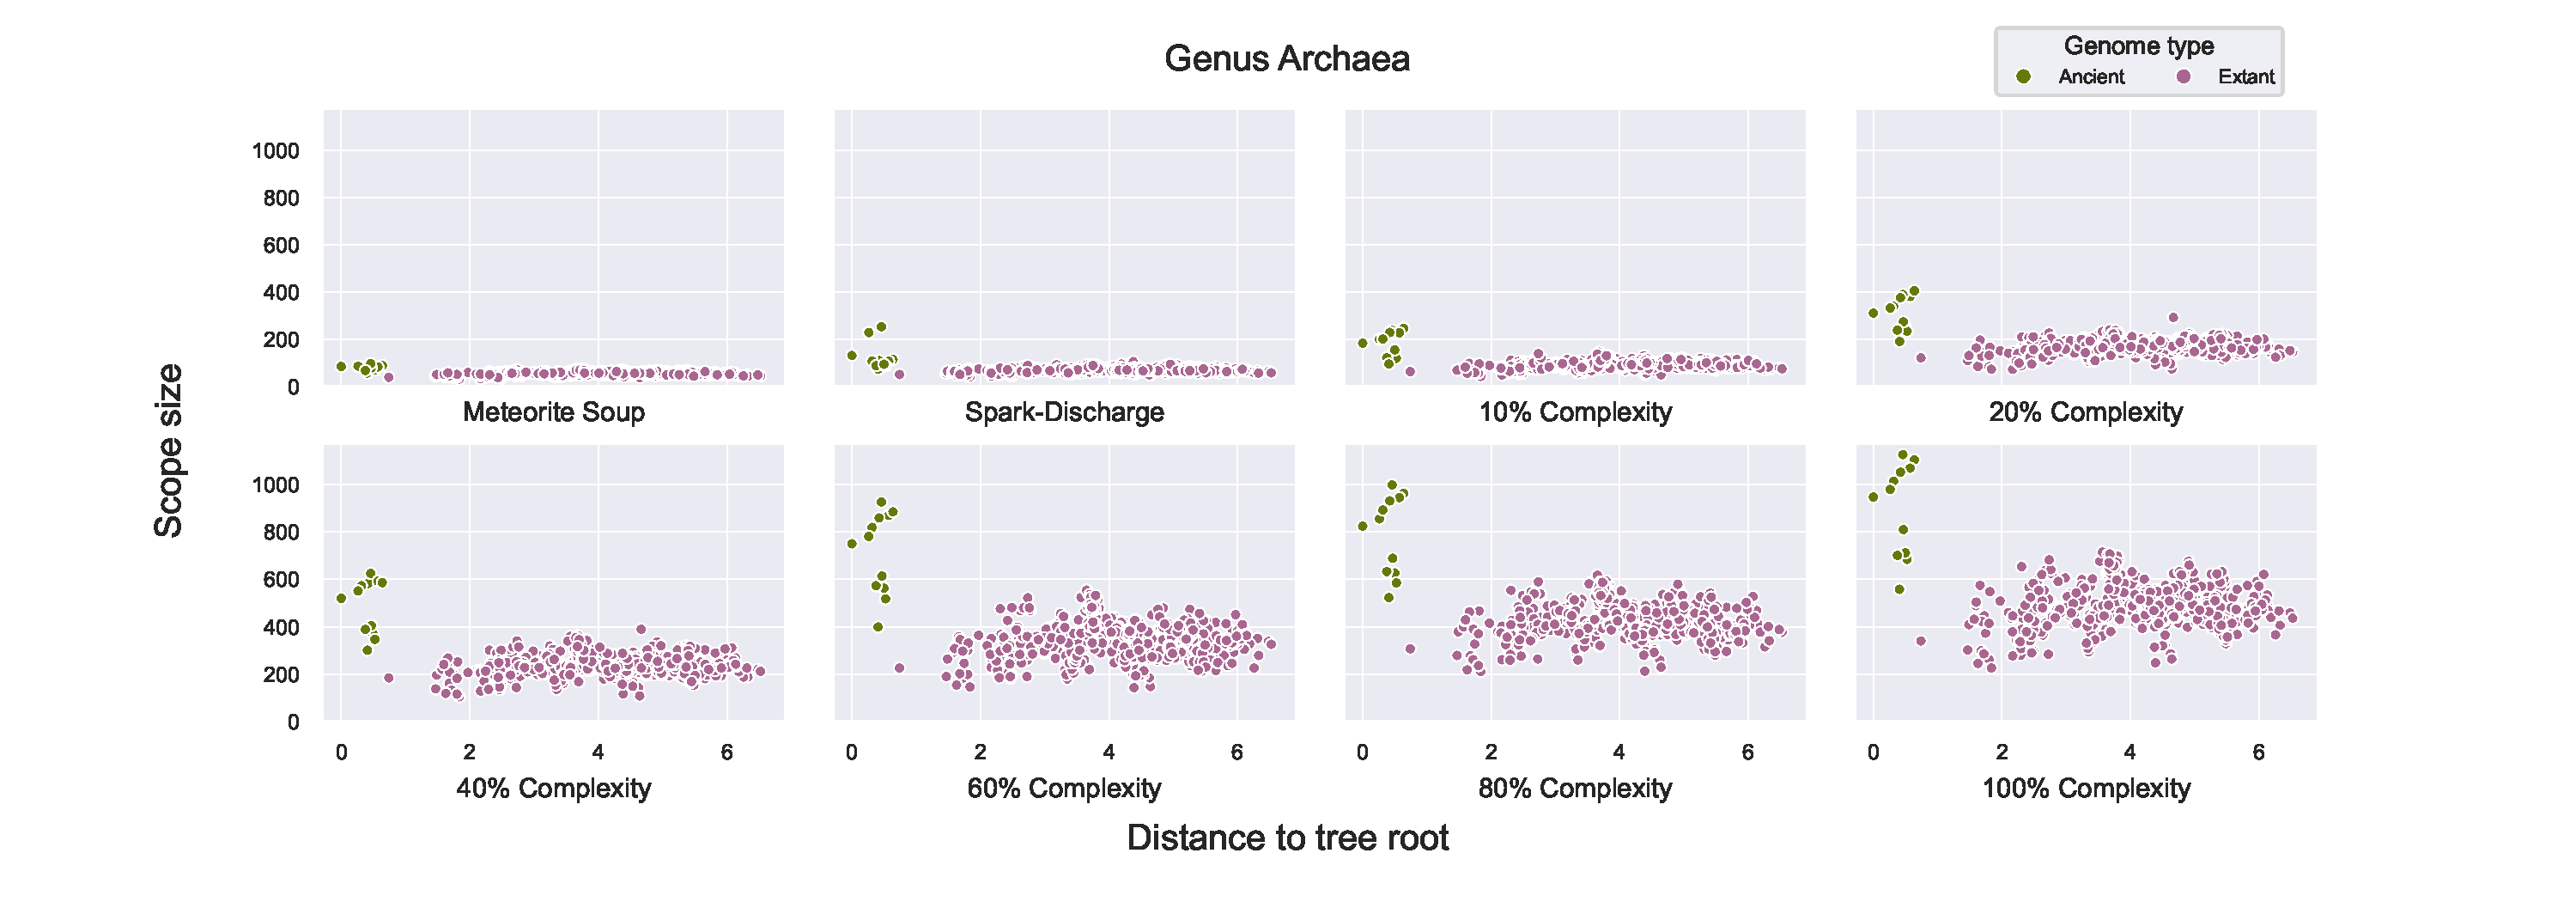
\includegraphics[width=0.95\textwidth]{scopesize_vs_disttoroot/gen4arc_ss_rootdist.pdf}
    \caption{Genus level archaea}
    \label{genarc_scopesize}
\end{figure}   

\begin{figure}[H]
    \centering
    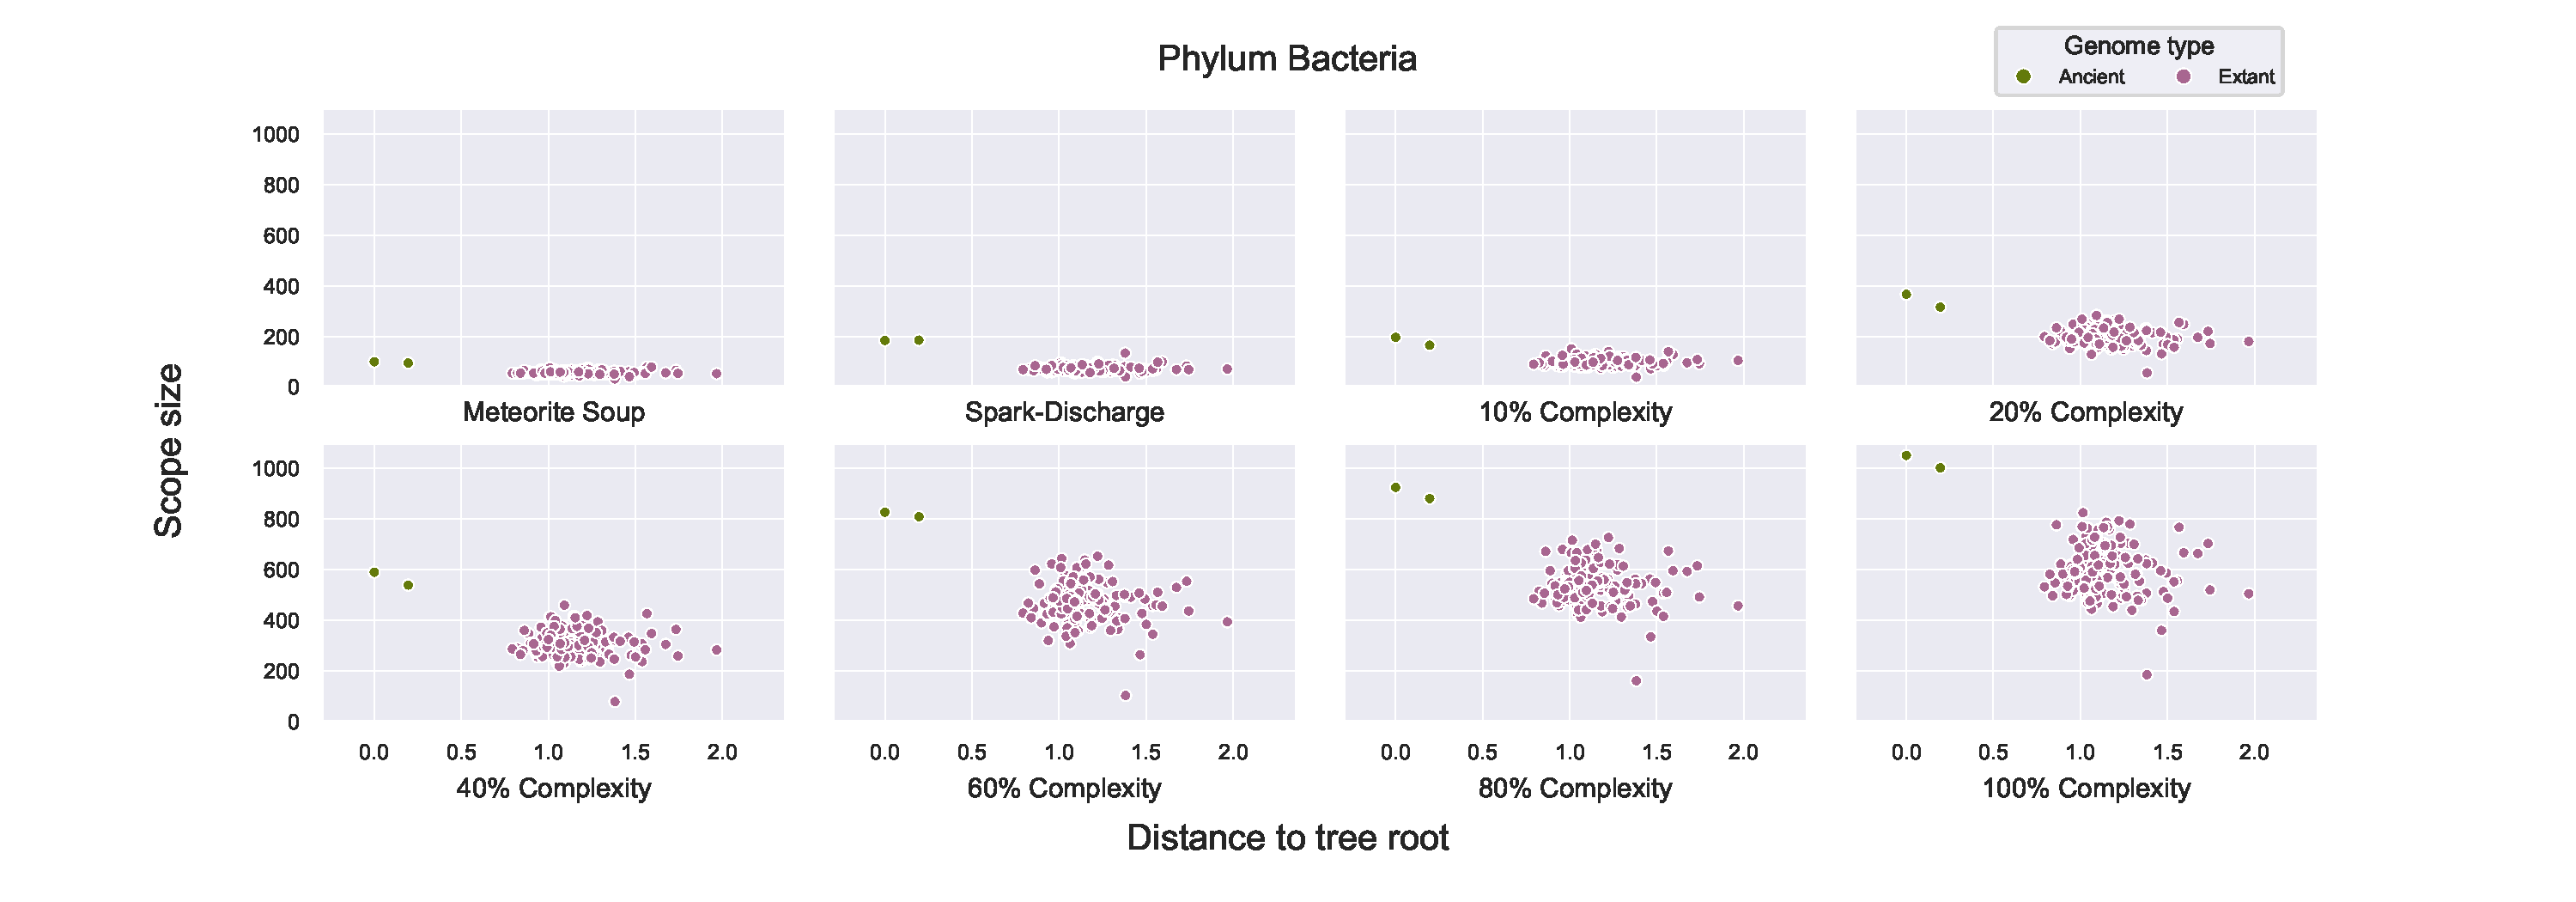
\includegraphics[width=0.95\textwidth]{scopesize_vs_disttoroot/phy4bac_ss_rootdist.pdf}
    \caption{Phylum level bacteria}
    \label{phybac_scopesize}
\end{figure}   

\begin{figure}[H]
    \centering
    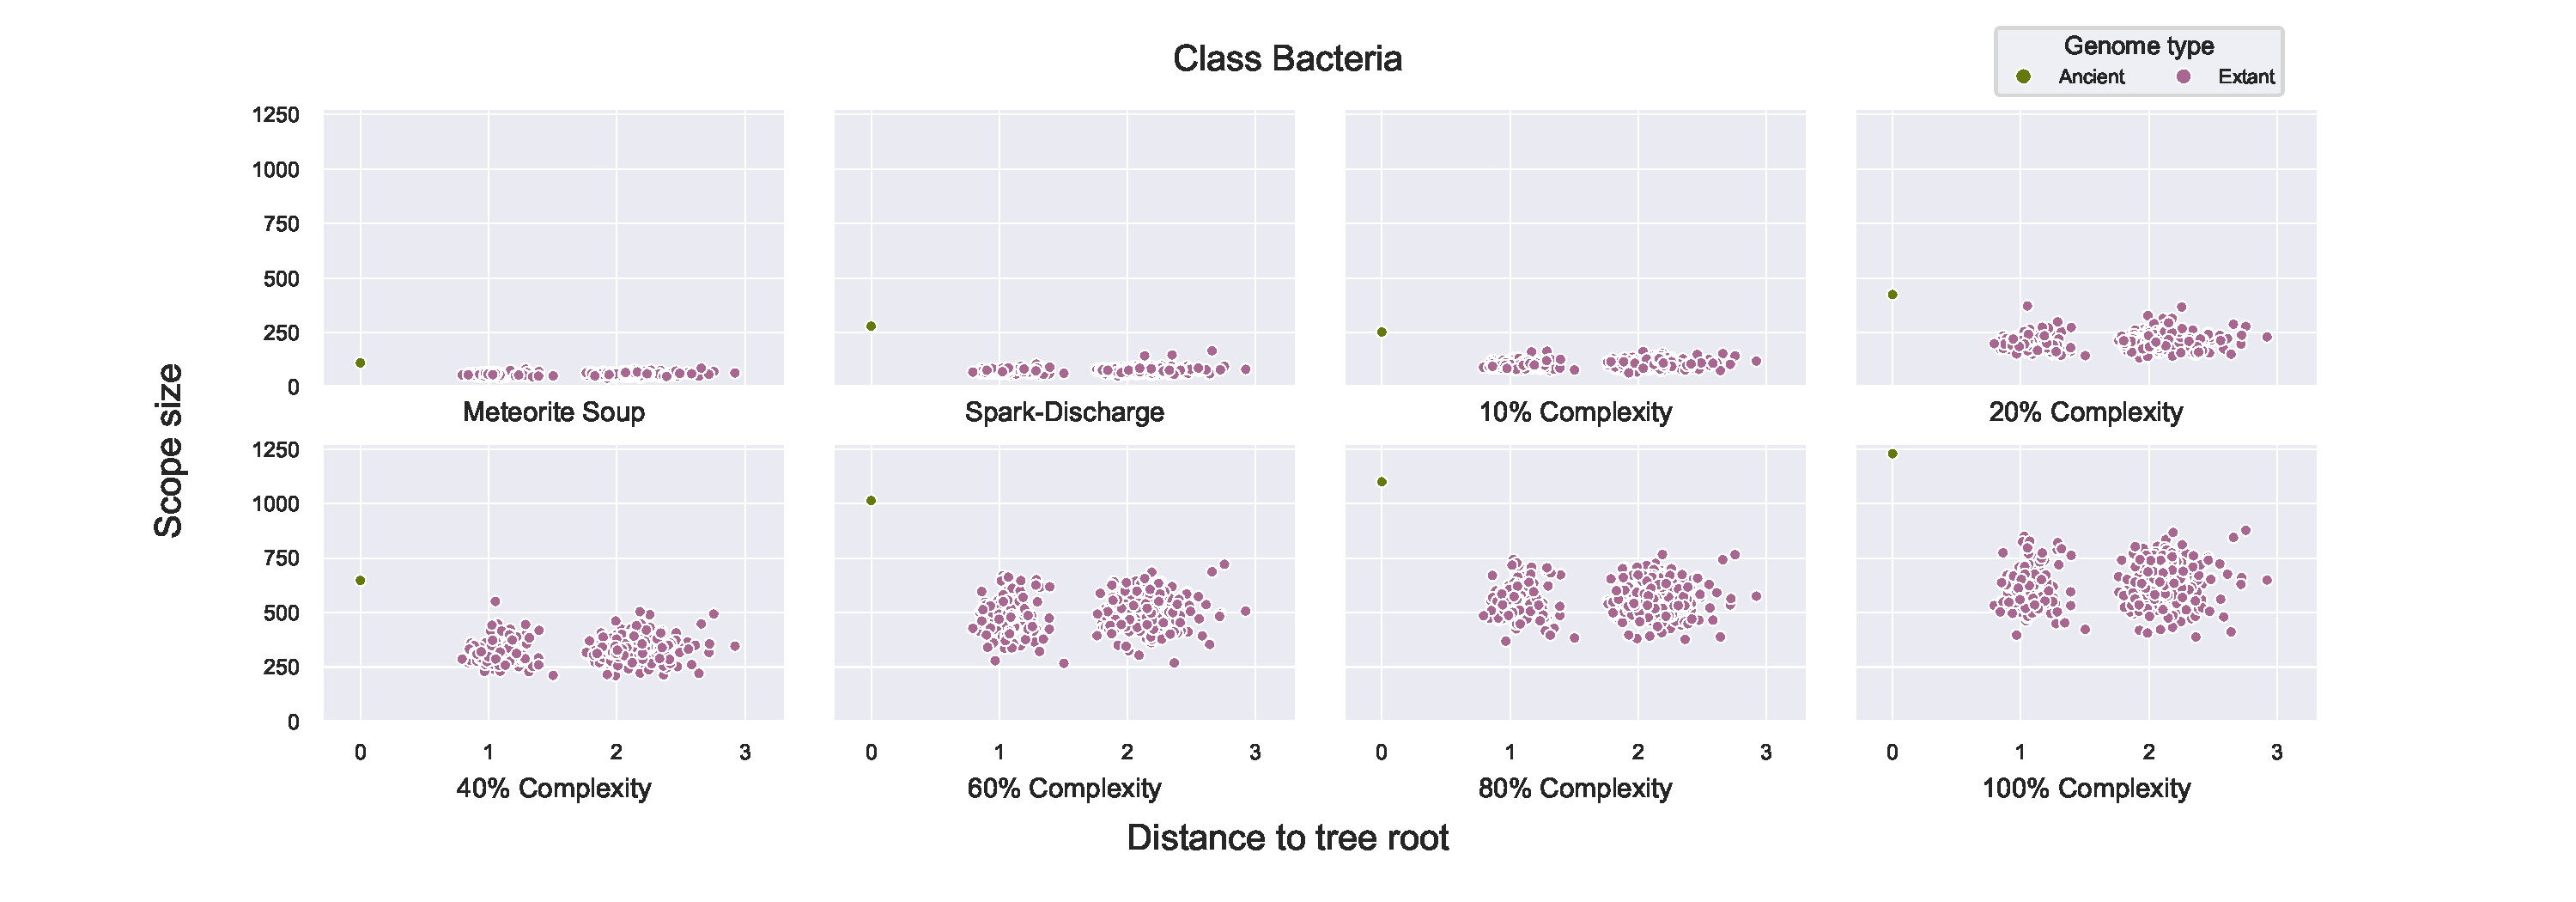
\includegraphics[width=0.95\textwidth]{scopesize_vs_disttoroot/cla4bac_ss_rootdist.pdf}
    \caption{Class level bacteria}
    \label{clabac_scopesize}
\end{figure}   




%\subsection*{A2. Metabolic Network Expansion}
%\addcontentsline{toc}{subsection}{Metabolic Network Expansion}






\end{document}

